\documentclass[11pt,a4paper]{article}
\usepackage[utf8]{inputenc}
\usepackage[T1]{fontenc}
\usepackage{lmodern}
\usepackage[brazil]{babel}
\usepackage[margin=2.3cm]{geometry}
\usepackage{amsmath,amssymb}
\usepackage{booktabs,array,graphicx,float,multirow}
\usepackage[table]{xcolor}
\usepackage{tcolorbox}
\usepackage{listings}
\usepackage{longtable}
\usepackage{hyperref}
\hypersetup{colorlinks=true,linkcolor=blue!50!black}
\setlength{\parindent}{0pt}\setlength{\parskip}{5pt}
\newcommand{\Vc}[1]{V_{c#1}}
\newcommand{\Vin}{V_{in}}
\newcommand{\pct}{\,\%}
\newcommand{\num}[1]{\mathrm{#1}}
\newtcolorbox{just}{colback=blue!4,colframe=blue!50!black,title=Por que isso?,fonttitle=\bfseries\small,boxrule=.5pt,left=4pt,right=4pt,top=2pt,bottom=2pt}
\newtcolorbox{res}{colback=green!5,colframe=green!40!black,title=Resultado,fonttitle=\bfseries\small,boxrule=.5pt,left=4pt,right=4pt,top=2pt,bottom=2pt}
\newtcolorbox{formula}{colback=orange!6,colframe=orange!60!black,title=Fórmula de partida,fonttitle=\bfseries\small,boxrule=.5pt,left=4pt,right=4pt,top=2pt,bottom=2pt}
\newtcolorbox{alerta}{colback=red!5,colframe=red!60!black,title=Atenção,fonttitle=\bfseries\small,boxrule=.5pt,left=4pt,right=4pt,top=2pt,bottom=2pt}
\newtcolorbox{todo}{colback=yellow!10,colframe=yellow!50!black,title=Experimento (a preencher na bancada),fonttitle=\bfseries\small,boxrule=.5pt,left=4pt,right=4pt,top=2pt,bottom=2pt}

\lstset{basicstyle=\ttfamily\fontsize{6.5}{7.8}\selectfont,breaklines=true,frame=single,columns=fullflexible,keepspaces=true,numbers=left,numberstyle=\tiny\color{gray},xleftmargin=1.2em,
 literate={á}{{\'a}}1 {é}{{\'e}}1 {í}{{\'i}}1 {ó}{{\'o}}1 {ú}{{\'u}}1 {ã}{{\~a}}1 {õ}{{\~o}}1 {ç}{{\c c}}1 {â}{{\^a}}1 {ê}{{\^e}}1 {ô}{{\^o}}1 {à}{{\`a}}1 {Á}{{\'A}}1 {É}{{\'E}}1 {Ç}{{\c C}}1 {º}{{\textdegree}}1 {→}{{->}}1 {≈}{{~}}1 {—}{{--}}1 {×}{{x}}1 {µ}{{u}}1 {Δ}{{D}}1 {≥}{{>=}}1 {≤}{{<=}}1 {±}{{+-}}1}

\begin{document}
\begin{center}
{\LARGE\bfseries Segunda Avaliação de Controle de Processos}\\[4pt]
{\Large Resolução detalhada, com os cálculos por extenso e os resultados experimentais da Questão 1}\\[8pt]
Aluno(a): Izabella Camops Trarbach\\
Prof.\ Saul da S.\ Munareto --- Engenharia de Controle e Automação --- IFES Serra\\
Circuito G; planta de controle: $\Vc3/\Vin$
\end{center}

\begin{tcolorbox}[colback=gray!6,colframe=gray!60]
\textbf{Como ler este documento.} Cada cálculo segue sempre a mesma ordem:
\textbf{(1)} a fórmula padrão (caixa laranja); \textbf{(2)} a modificação necessária para o nosso caso, com a justificativa (caixa azul);
\textbf{(3)} a substituição dos números, passo a passo; \textbf{(4)} o resultado (caixa verde).
Todas as grandezas estão em \% da escala (100\,\% $=5$ V do Arduino), e os tempos em segundos.
Os números intermediários foram arredondados só na apresentação; todas as contas foram refeitas por computador sem arredondar e conferidas.
Os resultados experimentais da Questão 1 (itens 1.1, 1.2 e 1.3) estão nas Seções~\ref{expdados} a \ref{conclq1}; os demais itens ainda têm caixas amarelas a preencher depois dos ensaios.
Para a parte da identificação (Seções 3 a 6), as tabelas que dependem do arquivo antigo \texttt{Tiago\_Izabella\_260921.csv} (instantes de 28,3\,\% etc.\ e erros RMS) foram tiradas do relatório original; os ensaios da Questão 1 (Seções~\ref{expdados} a \ref{conclq1}) foram analisados diretamente dos CSVs \texttt{Q11}, \texttt{Q12}, \texttt{Q13a} e \texttt{Q13b}, cujo código está no Apêndice~\ref{apcodigos}.
\end{tcolorbox}

\tableofcontents
\newpage
%==================== PARTE 1 ====================
\section{O circuito e os valores medidos}
O circuito é de três estágios RC acoplados, com $R_4$ ligado ao terra:
\[
\Vin \;-\; R_1 \;-\; \underbrace{\Vc1}_{C_1} \;-\; R_2 \;-\; \underbrace{\Vc2}_{C_2} \;-\; R_3 \;-\; \underbrace{\Vc3}_{C_3} \;-\; R_4 \;-\; \text{terra}
\]
Valores medidos com o multímetro:
\begin{center}
\begin{tabular}{cccc|ccc}
\toprule $R_1$ & $R_2$ & $R_3$ & $R_4$ & $C_1$ & $C_2$ & $C_3$\\ \midrule
22,0 k$\Omega$ & 46,8 k$\Omega$ & 32,6 k$\Omega$ & 66,8 k$\Omega$ & 947 $\mu$F & 947 $\mu$F & 955 $\mu$F\\ \bottomrule
\end{tabular}
\end{center}

\subsection{Condutâncias}
\begin{formula}\[ g_k=\frac{1}{R_k} \]\end{formula}
\begin{just}Trabalhar com condutâncias evita frações aninhadas: a corrente num resistor é simplesmente $g\cdot\Delta V$.\end{just}
\begin{align*}
g_1&=\frac{1}{22\,000}=45{,}455\ \mu\mathrm{S}, & g_2&=\frac{1}{46\,800}=21{,}368\ \mu\mathrm{S},\\
g_3&=\frac{1}{32\,600}=30{,}675\ \mu\mathrm{S}, & g_4&=\frac{1}{66\,800}=14{,}970\ \mu\mathrm{S}.
\end{align*}
Somas que vão aparecer nas equações (cada nó soma as condutâncias dos dois resistores ligados a ele):
\begin{align*}
A_1&=g_1+g_2=45{,}455+21{,}368=66{,}822\ \mu\mathrm{S}\\
A_2&=g_2+g_3=21{,}368+30{,}675=52{,}042\ \mu\mathrm{S}\\
A_3&=g_3+g_4=30{,}675+14{,}970=45{,}645\ \mu\mathrm{S}
\end{align*}

%------------------------------------------------------------------
\section{Modelo matemático completo (funções de transferência da 1ª avaliação)}
\subsection{Equações dos nós (leis de Kirchhoff das correntes)}
\begin{formula}
Em cada nó: \emph{corrente que chega pelo resistor da esquerda = corrente que vai ao capacitor + corrente que sai pelo resistor da direita}, com $i_C=C\,\dfrac{dv}{dt}$ e $i_R=\dfrac{\Delta V}{R}$.
\end{formula}
\begin{align}
C_1\dot V_{c1}&=\frac{\Vin-\Vc1}{R_1}-\frac{\Vc1-\Vc2}{R_2}\\
C_2\dot V_{c2}&=\frac{\Vc1-\Vc2}{R_2}-\frac{\Vc2-\Vc3}{R_3}\\
C_3\dot V_{c3}&=\frac{\Vc2-\Vc3}{R_3}-\frac{\Vc3-0}{R_4}
\end{align}
\begin{just}O nó 3 só tem $R_4$ para o terra (por isso a tensão do terra é 0). Não existe um quarto capacitor: o sistema tem 3 estados ($\Vc1,\Vc2,\Vc3$), logo é de 3ª ordem.\end{just}

\subsection{Transformada de Laplace}
\begin{just}O circuito é linear e invariante no tempo. Trabalhando com desvios em torno de um ponto de operação (condições iniciais nulas), a derivada vira multiplicação por $s$: $\dot V\to sV$. Isso transforma o sistema diferencial num sistema algébrico.\end{just}
Substituindo $1/R_k=g_k$ e agrupando os termos de cada tensão:
\begin{align*}
(C_1s+g_1+g_2)\,\Vc1-g_2\,\Vc2&=g_1\,\Vin\\
-g_2\,\Vc1+(C_2s+g_2+g_3)\,\Vc2-g_3\,\Vc3&=0\\
-g_3\,\Vc2+(C_3s+g_3+g_4)\,\Vc3&=0
\end{align*}
Definindo $a_{11}=C_1s+A_1$, $a_{22}=C_2s+A_2$, $a_{33}=C_3s+A_3$, em forma matricial $M(s)\mathbf V=\mathbf b\,\Vin$:
\[
\begin{bmatrix}a_{11}&-g_2&0\\-g_2&a_{22}&-g_3\\0&-g_3&a_{33}\end{bmatrix}
\begin{bmatrix}\Vc1\\\Vc2\\\Vc3\end{bmatrix}=\begin{bmatrix}g_1\\0\\0\end{bmatrix}\Vin .
\]

\subsection{Determinante $\Delta(s)=\det M(s)$ (polinômio característico)}
Expansão pela primeira linha:
\[
\Delta=a_{11}\,(a_{22}a_{33}-g_3^2)-(-g_2)\big[(-g_2)a_{33}-(-g_3)\cdot0\big]=a_{11}\,(a_{22}a_{33}-g_3^2)-g_2^2\,a_{33}.
\]
Chamo $P(s)=a_{22}a_{33}-g_3^2$ e expando $(C_2s+A_2)(C_3s+A_3)=C_2C_3s^2+(C_2A_3+C_3A_2)s+A_2A_3$:
\[
P(s)=P_2s^2+P_1s+P_0,\quad P_2=C_2C_3,\;\; P_1=C_2A_3+C_3A_2,\;\; P_0=A_2A_3-g_3^2 .
\]
Substituindo os valores (capacitâncias em F, condutâncias em S):
\begin{align*}
P_2&=947\!\times\!10^{-6}\cdot955\!\times\!10^{-6}=9{,}044\times10^{-7}\\
P_1&=947\!\times\!10^{-6}\cdot45{,}645\!\times\!10^{-6}+955\!\times\!10^{-6}\cdot52{,}042\!\times\!10^{-6}\\&=4{,}323\times10^{-8}+4{,}970\times10^{-8}=9{,}293\times10^{-8}\\
P_0&=52{,}042\!\times\!10^{-6}\cdot45{,}645\!\times\!10^{-6}-(30{,}675\!\times\!10^{-6})^2\\&=2{,}3755\times10^{-9}-9{,}410\times10^{-10}=1{,}435\times10^{-9}
\end{align*}
Agora $\Delta=(C_1s+A_1)P(s)-g_2^2(C_3s+A_3)$. Multiplicando e agrupando por potências de $s$: $\Delta=D_3s^3+D_2s^2+D_1s+D_0$,
\begin{align*}
D_3&=C_1P_2=947\!\times\!10^{-6}\cdot9{,}044\!\times\!10^{-7}=8{,}565\times10^{-10}\\
D_2&=C_1P_1+A_1P_2=8{,}800\times10^{-11}+6{,}043\times10^{-11}=1{,}484\times10^{-10}\\
D_1&=C_1P_0+A_1P_1-g_2^2C_3=1{,}358\times10^{-12}+6{,}210\times10^{-12}-4{,}360\times10^{-13}=7{,}132\times10^{-12}\\
D_0&=A_1P_0-g_2^2A_3=9{,}586\times10^{-14}-2{,}084\times10^{-14}=7{,}502\times10^{-14}
\end{align*}
(onde $g_2^2=4{,}566\times10^{-10}\ \mathrm{S^2}$).

\subsection{Numeradores pela regra de Cramer}
\begin{formula}$V_{cj}=\Delta_j/\Delta$, onde $\Delta_j$ é o determinante de $M$ com a coluna $j$ trocada por $\mathbf b\Vin=[g_1\Vin\ 0\ 0]^T$.\end{formula}
\textbf{$\Vc3$ (coluna 3 trocada).} Expandindo pela terceira coluna (só o 1º elemento é não nulo):
\[
\Delta_3=g_1\Vin\det\begin{bmatrix}-g_2&a_{22}\\0&-g_3\end{bmatrix}=g_1\Vin\,(g_2g_3)\ \Rightarrow\ \frac{\Vc3}{\Vin}=\frac{g_1g_2g_3}{\Delta(s)}.
\]
\textbf{$\Vc2$ (coluna 2 trocada).} Só o 1º elemento é não nulo, com sinal $-1$ (posição (1,2)):
\[
\Delta_2=-g_1\Vin\det\begin{bmatrix}-g_2&-g_3\\0&a_{33}\end{bmatrix}=-g_1\Vin(-g_2a_{33})=g_1g_2a_{33}\Vin\ \Rightarrow\ \frac{\Vc2}{\Vin}=\frac{g_1g_2(C_3s+A_3)}{\Delta(s)}.
\]
\textbf{$\Vc1$ (coluna 1 trocada).} Expandindo pela primeira coluna:
\[
\Delta_1=g_1\Vin\det\begin{bmatrix}a_{22}&-g_3\\-g_3&a_{33}\end{bmatrix}=g_1\Vin\,P(s)\ \Rightarrow\ \frac{\Vc1}{\Vin}=\frac{g_1P(s)}{\Delta(s)}.
\]
\begin{just}Os três quocientes têm o \emph{mesmo denominador} $\Delta(s)$: é o polinômio característico da matriz, e por isso as três tensões compartilham os mesmos polos. O que muda é o numerador (os zeros).\end{just}

\subsection{Normalização (termo constante igual a 1)}
\begin{just}A forma padrão de função de transferência para processos é $K\,\dfrac{\prod(\tau_{z}s+1)}{\prod(\tau_{p}s+1)}$: o termo independente de $s$ vale 1, e o ganho estático $K$ aparece explicitamente. Para chegar lá, divido numerador e denominador por $D_0$ (o termo independente de $\Delta$).\end{just}
\[
\frac{\Delta}{D_0}=\frac{D_3}{D_0}s^3+\frac{D_2}{D_0}s^2+\frac{D_1}{D_0}s+1=\frac{8{,}565\times10^{-10}}{7{,}502\times10^{-14}}s^3+\frac{1{,}484\times10^{-10}}{7{,}502\times10^{-14}}s^2+\frac{7{,}132\times10^{-12}}{7{,}502\times10^{-14}}s+1
\]
\[
D(s)=11\,416{,}7\,s^3+1978{,}65\,s^2+95{,}071\,s+1 .
\]
\begin{res}
\[\frac{\Vc3}{\Vin}=\frac{0{,}3971}{11\,416{,}7\,s^3+1978{,}65\,s^2+95{,}071\,s+1}\]
\[\frac{\Vc2}{\Vin}=\frac{0{,}5910\,(20{,}92\,s+1)}{D(s)},\qquad \frac{\Vc1}{\Vin}=\frac{0{,}8692\,(630{,}4\,s^2+64{,}78\,s+1)}{D(s)}\]
\end{res}
Como os numeradores foram obtidos:
\begin{itemize}
\item $\Vc3$: $\dfrac{g_1g_2g_3}{D_0}=\dfrac{45{,}455\cdot21{,}368\cdot30{,}675\times10^{-18}}{7{,}502\times10^{-14}}=\dfrac{2{,}979\times10^{-14}}{7{,}502\times10^{-14}}=0{,}3971$.
\item $\Vc2$: $\dfrac{g_1g_2(C_3s+A_3)}{D_0}=\dfrac{g_1g_2A_3}{D_0}\left(\dfrac{C_3}{A_3}s+1\right)$; $\dfrac{g_1g_2A_3}{D_0}=\dfrac{4{,}433\times10^{-14}}{7{,}502\times10^{-14}}=0{,}5910$ e $\dfrac{C_3}{A_3}=\dfrac{955\times10^{-6}}{45{,}645\times10^{-6}}=20{,}92$ s.
\item $\Vc1$: $\dfrac{g_1P(s)}{D_0}=\dfrac{g_1P_0}{D_0}\left(\dfrac{P_1}{P_0}s+\dfrac{P_2}{P_0}s^2+1\right)$; $\dfrac{g_1P_0}{D_0}=\dfrac{6{,}520\times10^{-14}}{7{,}502\times10^{-14}}=0{,}8692$, $\dfrac{P_1}{P_0}=\dfrac{9{,}293\times10^{-8}}{1{,}435\times10^{-9}}=64{,}78$, $\dfrac{P_2}{P_0}=\dfrac{9{,}044\times10^{-7}}{1{,}435\times10^{-9}}=630{,}4$.
\end{itemize}

\subsection{Ganhos estáticos (duas conferências)}
O ganho estático é $G(0)$. Pelo método anterior: $K_3=0{,}3971$, $K_2=0{,}5910$, $K_1=0{,}8692$.

\textbf{Conferência por divisores resistivos.} Em regime permanente os capacitores são circuitos abertos (corrente nula), então a mesma corrente $\Vin/R_t$ percorre todos os resistores, com $R_t=R_1+R_2+R_3+R_4=22+46{,}8+32{,}6+66{,}8=168{,}2$ k$\Omega$:
\[\begin{gathered}
K_3=\frac{R_4}{R_t}=\frac{66{,}8}{168{,}2}=0{,}3971,\\
K_2=\frac{R_3+R_4}{R_t}=\frac{99{,}4}{168{,}2}=0{,}5910,\\
K_1=\frac{R_2+R_3+R_4}{R_t}=\frac{146{,}2}{168{,}2}=0{,}8692 .
\end{gathered}\]
Os dois caminhos coincidem, o que confirma o modelo.

\subsection{Polos, zeros e constantes de tempo}
As raízes de $D(s)=0$ (cúbica, resolvida numericamente) são
$s_1=-0{,}01456$, $s_2=-0{,}06250$, $s_3=-0{,}09625$ s$^{-1}$.
\begin{formula}Cada polo real $s=-1/\tau_i$ dá uma constante de tempo $\tau_i=-1/s$; o denominador fatora em $(\tau_1s+1)(\tau_2s+1)(\tau_3s+1)$.\end{formula}
\[
\tau_1=\frac{1}{0{,}01456}=68{,}68\ \mathrm{s},\qquad \tau_2=\frac{1}{0{,}06250}=16{,}00\ \mathrm{s},\qquad \tau_3=\frac{1}{0{,}09625}=10{,}39\ \mathrm{s}.
\]
\textbf{Verificação pelas relações de Vieta} (coeficientes do produto $(\tau_1s+1)(\tau_2s+1)(\tau_3s+1)$ devem ser os de $D(s)$):
\begin{align*}
\tau_1+\tau_2+\tau_3&=68{,}68+16{,}00+10{,}39=95{,}07\ \ \checkmark\ (\text{coef. de }s)\\
\tau_1\tau_2+\tau_1\tau_3+\tau_2\tau_3&=1098{,}9+713{,}6+166{,}2=1978{,}7\ \ \checkmark\ (\text{coef. de }s^2)\\
\tau_1\tau_2\tau_3&=68{,}68\cdot16{,}00\cdot10{,}39=11\,416{,}7\ \ \checkmark\ (\text{coef. de }s^3)
\end{align*}
Todas as raízes são reais e negativas $\Rightarrow$ sistema estável e \textbf{sobreamortecido} (sem oscilação). A constante \emph{dominante} é $\tau_1=68{,}68$ s (a maior; é $68{,}68/16{,}00=4{,}29$ vezes a segunda).

\textbf{Zeros (constantes de tempo de avanço):}
\begin{itemize}
\item $\Vc3$: o numerador é constante $\Rightarrow$ não há zeros.
\item $\Vc2$: o zero é a raiz de $C_3s+A_3=0$, isto é, $\tau_z=C_3/A_3=20{,}92$ s.
\item $\Vc1$: os zeros são as raízes de $630{,}4s^2+64{,}78s+1=0$. Por Bhaskara:
\[
\Delta=64{,}78^2-4\cdot630{,}4\cdot1=4196{,}4-2521{,}6=1674{,}8,\quad\sqrt\Delta=40{,}92,
\]
\[
s=\frac{-64{,}78\pm40{,}92}{2\cdot630{,}4}\ \Rightarrow\ s_{z1}=-0{,}01892,\ s_{z2}=-0{,}08383\ \Rightarrow\ \tau_{z1}=52{,}85\ \mathrm{s},\ \tau_{z2}=11{,}93\ \mathrm{s}.
\]
Conferência: $52{,}85\cdot11{,}93=630{,}5$ e $52{,}85+11{,}93=64{,}78$ $\checkmark$.
\end{itemize}
\begin{res}
\begin{align}
\frac{\Vc3}{\Vin}&=\frac{0{,}3971}{(68{,}68s+1)(16{,}00s+1)(10{,}39s+1)}\label{ft3}\\
\frac{\Vc2}{\Vin}&=\frac{0{,}5910\,(20{,}92s+1)}{(68{,}68s+1)(16{,}00s+1)(10{,}39s+1)}\\
\frac{\Vc1}{\Vin}&=\frac{0{,}8692\,(52{,}85s+1)(11{,}93s+1)}{(68{,}68s+1)(16{,}00s+1)(10{,}39s+1)}
\end{align}
\end{res}
\begin{just}\textbf{Tipo de curva previsto pelo grau relativo} (polos $-$ zeros): $\Vc1$ tem $3-2=1$, então a derivada em $t=0^+$ é diferente de zero e a curva tem inclinação máxima logo no início (\textbf{curva tipo C}). $\Vc2$ tem $3-1=2$ e $\Vc3$ tem $3-0=3$: a inclinação inicial é nula e há ponto de inflexão (\textbf{curva tipo S}). Isso diz de antemão qual método de redução usar em cada tensão. O sistema é \emph{interativo}: as constantes de tempo (10,4; 16,0; 68,7 s) são bem diferentes das de cada estágio isolado ($R_1C_1=20{,}8$ s etc.), porque cada capacitor carrega e descarrega os vizinhos.\end{just}

\subsection{Resposta ao degrau da FT completa (frações parciais)}
\begin{formula}Para $u=U\cdot1(t)$ e $G(s)=K\dfrac{\prod_k(\tau_{z,k}s+1)}{\prod_i(\tau_is+1)}$ com polos distintos:
\[
y(t)=K\Big[1-\sum_{i=1}^{3}c_i\,e^{-t/\tau_i}\Big],\qquad c_i=\frac{\prod_k\left(1-\tau_{z,k}/\tau_i\right)}{\prod_{j\ne i}\left(1-\tau_j/\tau_i\right)}\quad(U=1).\]
\end{formula}
\begin{just}O resíduo da exponencial em $s=-1/\tau_i$ é obtido multiplicando $Y(s)$ por $(\tau_is+1)$ e calculando em $s=-1/\tau_i$. Em $s=0$ o resíduo é $K$ (valor final). Como $y(0)=0$, deve valer $\sum c_i=1$ --- é a conferência.\end{just}
Exemplo detalhado: $\Vc3$, $c_1$ (polo $\tau_1=68{,}68$):
\[
c_1=\frac{1}{(1-\tau_2/\tau_1)(1-\tau_3/\tau_1)}=\frac{1}{(1-0{,}2329)(1-0{,}1513)}=\frac{1}{0{,}7671\cdot0{,}8487}=1{,}536 .
\]
Exemplo $\Vc2$, $c_1$ (numerador com $\tau_z=20{,}92$): $c_1=\dfrac{1-20{,}92/68{,}68}{0{,}7671\cdot0{,}8487}=\dfrac{0{,}6954}{0{,}6510}=1{,}068$. Os demais coeficientes seguem o mesmo procedimento:
\begin{center}
\begin{tabular}{lccc}\toprule & $c_1$ ($\tau_1=68{,}7$) & $c_2$ ($\tau_2=16{,}0$) & $c_3$ ($\tau_3=10{,}4$)\\\midrule
$\Vc3$ & $1{,}5360$ & $-0{,}8662$ & $0{,}3302$\\ $\Vc2$ & $1{,}0681$ & $0{,}2666$ & $-0{,}3347$\\ $\Vc1$ & $0{,}2926$ & $0{,}5075$ & $0{,}1999$\\\bottomrule
\end{tabular}
\end{center}
Conferência $\sum c_i=1$ em cada linha (p.\,ex.\ $\Vc3$: $1{,}5360-0{,}8662+0{,}3302=1{,}0000$). Esta expressão é a ``resposta da FT completa'' usada nas comparações.

%------------------------------------------------------------------
\section{Teste ao degrau experimental}
\subsection{O arquivo e o trecho usado}
O ScadaBR gravou uma amostra por segundo de cinco variáveis (1440 amostras cada): $SO=\Vin$, $VP=\Vc3$, $VP1=\Vc2$, $VP2=\Vc1$ (e $SP$). A entrada \texttt{SO} fica em 30\,\% nos primeiros 41 s, em 70\,\% até $t=577$ s e depois em 50\,\% até o fim. Para identificar as FTs reduzidas usei \textbf{apenas o degrau de 70\,\% para 50\,\%}:
\[
\Delta U=U_1-U_0=50{,}000-70{,}001=-20{,}000\,\%\ (\approx-1\ \mathrm{V}),\qquad t_{degrau}=576{,}5\ \mathrm{s}.
\]
\begin{just}O degrau começa de um regime permanente real (o patamar de 70\,\% dura 535 s, mais de $7\tau_1=481$ s) e termina em outro patamar longo (863 s). Assim $y_i$ e $y_f$ são confiáveis e não há transitório de teste anterior contaminando. Como o circuito é linear, o resultado vale para qualquer ponto de operação e para degraus em qualquer sentido.\end{just}
\begin{figure}[H]\centering
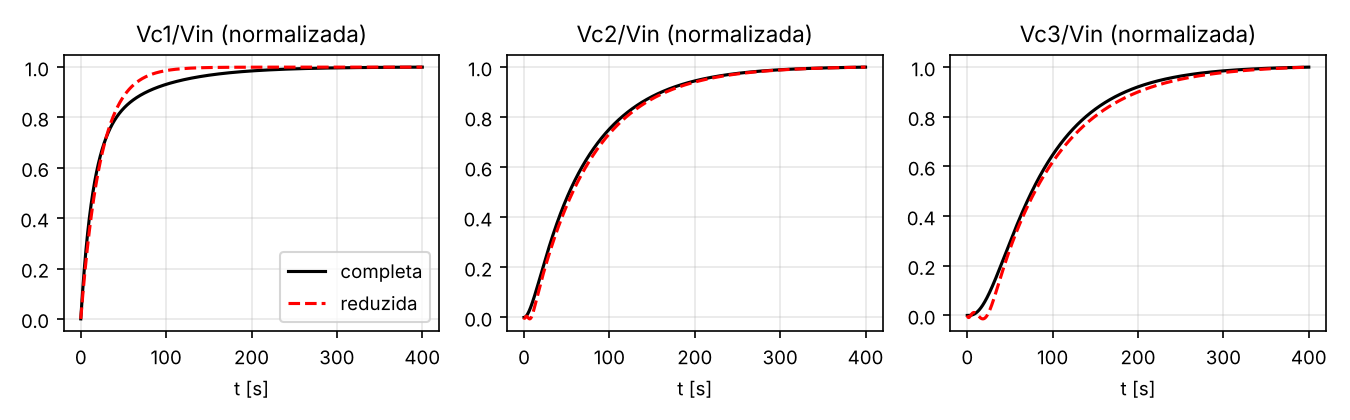
\includegraphics[width=.8\textwidth]{figs/steps.png}
\caption{Respostas ao degrau normalizadas das FTs completas (preto) e das reduzidas (vermelho tracejado), calculadas neste documento.}\end{figure}

\subsection{Tratamento dos dados}
\begin{formula}
$\displaystyle y_n(t)=\frac{y(t)-y_i}{y_f-y_i}$ (resposta normalizada, vai de 0 a 1);\qquad $\displaystyle K=\frac{y_f-y_i}{\Delta U}$.
\end{formula}
\begin{just}Normalizar elimina o sinal negativo do degrau (queda de 70 para 50) e permite aplicar as fórmulas dos métodos como se fosse um degrau positivo unitário. $y_i$ é a média das 128 amostras antes do degrau; $y_f$, a média das 150 últimas amostras (médias reduzem o ruído de quantização do ADC de 10 bits, resolução $100/1024=0{,}0977\,\%$).\end{just}
\begin{center}
\begin{tabular}{lccc}\toprule & $\Vc1$ & $\Vc2$ & $\Vc3$\\\midrule
$y_i$ [\%] (SO=70\,\%) & 60,774 & 41,104 & 27,454\\
$y_f$ [\%] (SO=50\,\%) & 43,431 & 29,382 & 19,618\\
$y_f-y_i$ [\%] & $-17{,}343$ & $-11{,}723$ & $-7{,}836$\\\bottomrule
\end{tabular}
\end{center}
\[
K_1=\frac{-17{,}343}{-20}=0{,}8671,\qquad K_2=\frac{-11{,}723}{-20}=0{,}5861,\qquad K_3=\frac{-7{,}836}{-20}=0{,}3918 .
\]
\textbf{Conferência pelo patamar final:} $y_f/50$: $43{,}431/50=0{,}8686$; $29{,}382/50=0{,}5876$; $19{,}618/50=0{,}3924$ (praticamente iguais, confirmando linearidade: saída nula para entrada nula).
\textbf{Comparação com a teoria:} o ganho medido fica 0,2\,\% a 1,3\,\% abaixo ($0{,}8671$ vs.\ $0{,}8692$; $0{,}5861$ vs.\ $0{,}5910$; $0{,}3918$ vs.\ $0{,}3971$), coerente com as tolerâncias dos $R$ e $C$, a quantização do ADC e a resistência de saída do Arduino. Adoto $K=(y_f-y_i)/\Delta U$, de modo que a FT reduzida termina exatamente no valor final medido.

\subsection{Instantes de 28,3\,\%, 35,3\,\%, 63,2\,\% e 85,3\,\%}
\begin{formula}Para cada nível $q$, procuro a primeira amostra $k+1$ com $y_n\ge q$ e interpolo linearmente entre $k$ e $k+1$:
\[t_q=t_k+\frac{q-y_{n,k}}{y_{n,k+1}-y_{n,k}}(t_{k+1}-t_k).\]\end{formula}
Exemplo completo ($\Vc3$, $q=0{,}632$): $t_k=103{,}5$ s ($y_{n,k}=0{,}6264$) e $t_{k+1}=104{,}5$ s ($y_{n,k+1}=0{,}6388$):
\[
t_{63,2}=103{,}5+\frac{0{,}632-0{,}6264}{0{,}6388-0{,}6264}\,(104{,}5-103{,}5)=103{,}5+\frac{0{,}0056}{0{,}0124}\cdot1=103{,}5+0{,}45=103{,}95\ \mathrm{s}.
\]
Resultados (em segundos desde o degrau):
\begin{center}
\begin{tabular}{lcccc}\toprule & $t_{28,3}$ & $t_{35,3}$ & $t_{63,2}$ & $t_{85,3}$\\\midrule
$\Vc1$ & 7,16 & 9,31 & 23,31 & 58,39\\ $\Vc2$ & 32,34 & 39,12 & 78,26 & 146,80\\ $\Vc3$ & 51,93 & 60,55 & 103,95 & 173,70\\\bottomrule
\end{tabular}
\end{center}

%------------------------------------------------------------------
\section{Redução a ganho, constante de tempo e atraso}
\subsection{O modelo reduzido e a origem dos métodos}
\begin{formula}Modelo de 1ª ordem com atraso (FOPDT): $\displaystyle G(s)=\frac{K\,e^{-t_0s}}{\tau s+1}$. Sua resposta ao degrau é $y_n(t)=1-e^{-(t-t_0)/\tau}$ para $t\ge t_0$ (e $0$ antes).\end{formula}
Cada método de identificação vem de impor que essa curva passe por pontos da curva real. Vou deduzir as constantes numéricas para entender de onde saem.

\textbf{Curva tipo C} (sem inflexão, inclinação máxima na origem; caso de $\Vc1$): não há atraso, $t_0=0$, e em $t=\tau$ a resposta vale $1-e^{-1}=0{,}632$. Logo $\tau=t_{63,2}$.

\textbf{Curva tipo S, método de Smith (Ajuste 3, seção 7-2.1 do livro).} Impondo que a FOPDT passe pelos pontos de 28,3\,\% e 63,2\,\%:
\[\begin{gathered}
1-e^{-(t_{28,3}-t_0)/\tau}=0{,}283\ \Rightarrow\ \frac{t_{28,3}-t_0}{\tau}=-\ln(0{,}717)=0{,}333\approx\frac13,\\
1-e^{-(t_{63,2}-t_0)/\tau}=0{,}632\ \Rightarrow\ \frac{t_{63,2}-t_0}{\tau}=1 .
\end{gathered}\]
Subtraindo: $t_{63,2}-t_{28,3}=\tau(1-\tfrac13)=\tfrac23\tau$. Logo
\[
\boxed{\tau=1{,}5\,(t_{63,2}-t_{28,3}),\qquad t_0=t_{63,2}-\tau .}
\]
\textbf{Método de Sundaresan--Krishnaswamy} (mesmo raciocínio com 35,3\,\% e 85,3\,\%):
$\frac{t_{35,3}-t_0}{\tau}=-\ln(0{,}647)=0{,}435$ e $\frac{t_{85,3}-t_0}{\tau}=-\ln(0{,}147)=1{,}917$. Subtraindo: $t_{85,3}-t_{35,3}=1{,}482\tau$, logo $\tau=0{,}675\,(t_{85,3}-t_{35,3})\approx0{,}67(t_{85,3}-t_{35,3})$ e $t_0=t_{35,3}-0{,}435\tau=1{,}3\,t_{35,3}-0{,}29\,t_{85,3}$.

\textbf{Método da tangente no ponto de inflexão (Ziegler--Nichols, Ajuste 1).} Acho o ponto de maior inclinação $(t_i,y_i)$ com inclinação $m$. A reta tangente $y=y_i+m(t-t_i)$ corta o eixo do tempo ($y=0$) em $t_0=t_i-y_i/m$ e atinge o valor final ($y=1$) em $t=t_i+(1-y_i)/m$; então $\tau=\big[t_i+(1-y_i)/m\big]-t_0$.

\subsection{Contas, passo a passo}
\textbf{$\Vc1$ (tipo C).} A inclinação máxima ocorre na primeira amostra ($m=0{,}0500$ s$^{-1}$; a derivada teórica em $0^+$ é $0{,}048$ s$^{-1}$, ver Lista 2). Então $t_0=0$ e $\tau=t_{63,2}=23{,}31$ s. \emph{Teste de coerência:} se eu tentasse Smith, $\tau=1{,}5(23{,}31-7{,}16)=24{,}23$ s e $t_0=23{,}31-24{,}23=-0{,}92$ s: atraso \emph{negativo}, sem sentido físico (a saída não antecipa a entrada), o que confirma que não há atraso.

\textbf{$\Vc2$ (tipo S), Smith:}
\[
\tau=1{,}5\,(78{,}26-32{,}34)=1{,}5\cdot45{,}92=68{,}88\ \mathrm{s},\qquad t_0=78{,}26-68{,}88=9{,}38\ \mathrm{s}.
\]
\textbf{$\Vc3$ (tipo S), Smith:}
\[
\tau=1{,}5\,(103{,}95-51{,}93)=1{,}5\cdot52{,}02=78{,}03\ \mathrm{s},\qquad t_0=103{,}95-78{,}03=25{,}92\ \mathrm{s}.
\]
\textbf{Sundaresan:} $\Vc2$: $\tau=0{,}67(146{,}80-39{,}12)=72{,}15$ s, $t_0=1{,}3\cdot39{,}12-0{,}29\cdot146{,}80=50{,}86-42{,}57=8{,}29$ s. $\Vc3$: $\tau=0{,}67(173{,}70-60{,}55)=75{,}81$ s, $t_0=1{,}3\cdot60{,}55-0{,}29\cdot173{,}70=78{,}72-50{,}37=28{,}35$ s.

\textbf{Tangente} (pontos de inflexão medidos): $\Vc2$: $t_i=22{,}5$, $y_i=0{,}178$, $m=0{,}01151$ s$^{-1}$: $t_0=22{,}5-0{,}178/0{,}01151=7{,}07$ s; $\tau=\big[22{,}5+(1-0{,}178)/0{,}01151\big]-7{,}07=93{,}93-7{,}07=86{,}86$ s. $\Vc3$: $t_i=43{,}5$, $y_i=0{,}213$, $m=0{,}00884$: $t_0=43{,}5-24{,}10=19{,}38$ s; $\tau=\big[43{,}5+0{,}787/0{,}00884\big]-19{,}38=132{,}5-19{,}38=113{,}10$ s.

\subsection{Resultados e escolha do método}
\begin{center}\small
\begin{tabular}{lccc}\toprule $\tau/t_0$ [s] & $\Vc1$ & $\Vc2$ & $\Vc3$\\\midrule
Tipo C ($\tau=t_{63,2}$, $t_0=0$) & \textbf{23,3 / 0,0} & 78,3 / 0,0 & 104,0 / 0,0\\
Smith (28,3/63,2) & 24,2 / $-0{,}9$ & \textbf{68,9 / 9,4} & \textbf{78,0 / 25,9}\\
Sundaresan (35,3/85,3) & 32,9 / $-4{,}8$ & 72,1 / 8,3 & 75,8 / 28,3\\
Tangente (Z--N) & 20,0 / 0,6 & 86,9 / 7,1 & 113,1 / 19,4\\
Mínimos quadrados (referência) & 27,0 / 0,0 & 72,1 / 7,5 & 79,7 / 23,4\\\bottomrule
\end{tabular}\end{center}
Para comparar os modelos com o experimento uso o erro RMS e o erro máximo, em \% do degrau:
\[
\begin{gathered}\varepsilon_{rms}=100\sqrt{\frac1N\sum_{k=1}^{N}\big(y_{mod,n}(t_k)-y_{exp,n}(t_k)\big)^2},\\
\varepsilon_{max}=100\max_k|y_{mod,n}(t_k)-y_{exp,n}(t_k)|,\quad 0<t<520\,\mathrm{s}\ (N=520).\end{gathered}
\]
RMS (máximo), vindos do relatório original com os dados:
\begin{center}\small
\begin{tabular}{lccc}\toprule & $\Vc1$ & $\Vc2$ & $\Vc3$\\\midrule
Tipo C & 2,87 (7,3) & 1,89 (8,5) & 4,89 (15,6)\\
Smith & 2,71 (6,8) & 0,71 (4,1) & 1,12 (7,1)\\
Sundaresan & 3,28 (13,3) & 0,53 (3,2) & 1,45 (9,1)\\
Tangente & 3,67 (9,4) & 3,55 (7,5) & 6,71 (12,6)\\
Mínimos quadrados & 2,48 (7,2) & 0,44 (2,6) & 0,97 (5,3)\\
FT completa & 0,73 (3,5) & 1,48 (3,2) & 1,75 (3,6)\\\bottomrule
\end{tabular}\end{center}
\begin{just}\textbf{$\Vc1$:} é curva tipo C (Smith dá atraso negativo), logo $\tau=t_{63,2}$ e $t_0=0$. \textbf{$\Vc2$ e $\Vc3$:} adoto Smith porque (i) é o método do livro (Ajuste 3); (ii) usa dois pontos no meio da subida, pouco sensíveis à quantização e ao valor final; (iii) seu erro RMS fica próximo ao dos mínimos quadrados (o melhor possível para uma FOPDT). A tangente é a pior (RMS 6,7\,\% em $\Vc3$): a inclinação máxima de um sistema de 3ª ordem é muito sensível à suavização dos dados. Tratar $\Vc3$ como curva C (RMS 4,9\,\%) também é ruim, o que confirma que ela é do tipo S.\end{just}
\textbf{Conferência independente (regra prática do livro, p.\,216):} $\tau\approx$ maior constante de tempo, $t_0\approx$ soma das menores. Com a Seção 2: $\tau\approx68{,}7$ s e $t_0\approx16{,}0+10{,}4=26{,}4$ s, próximo do identificado para $\Vc3$ ($78{,}0$ s e $25{,}9$ s).
\begin{res}
\[
\frac{\Vc1}{\Vin}\approx\frac{0{,}867}{23{,}3s+1},\qquad
\frac{\Vc2}{\Vin}\approx\frac{0{,}586\,e^{-9{,}4s}}{68{,}9s+1},\qquad
\frac{\Vc3}{\Vin}\approx\frac{0{,}392\,e^{-25{,}9s}}{78{,}0s+1}\ \ \text{(a planta de controle)}
\]
\end{res}

%------------------------------------------------------------------
\section{Comparação das respostas ao degrau}
A figura da Seção 3 já mostra as respostas normalizadas; os erros RMS acima quantificam: a FT completa acompanha o experimento com RMS de 0,7\,\% a 1,7\,\% do degrau (valida o modelo físico e as medidas de $R$ e $C$); a reduzida erra mais (2,9\,\% em $\Vc1$, 0,7\,\% em $\Vc2$, 1,1\,\% em $\Vc3$), o que é esperado: troca 3 polos (e zeros) por 1 polo e 1 atraso. Em $\Vc3$ e $\Vc2$ a reduzida reproduz o atraso inicial e a subida; a maior diferença está na cauda, pois o 1º ordem não representa o peso diferente do polo lento ($\tau_1=68{,}7$ s). Em $\Vc1$ a reduzida fica próxima da curva real até $\sim$20 s, cruza e depois fica acima, porque $\Vc1$ não é naturalmente de 1ª ordem (tem 3 polos e 2 zeros).

%------------------------------------------------------------------
\section{Diagramas de Bode e margens}
\subsection{Respostas em frequência}
\begin{formula}Substituindo $s=j\omega$ em $G(s)=K\prod(\tau_{z}s+1)/\prod(\tau_ps+1)$ e $G_{red}=Ke^{-t_0s}/(\tau s+1)$:
\[
|G_{compl}(j\omega)|=K\frac{\prod_k\sqrt{1+(\omega\tau_{z,k})^2}}{\prod_i\sqrt{1+(\omega\tau_i)^2}},\qquad
\angle G_{compl}=\sum_k\arctan(\omega\tau_{z,k})-\sum_i\arctan(\omega\tau_i),
\]
\[
|G_{red}(j\omega)|=\frac{K}{\sqrt{1+(\omega\tau)^2}},\qquad\angle G_{red}=-\arctan(\omega\tau)-\omega t_0\ (\text{rad}).
\]\end{formula}
\begin{just}O módulo de $(\tau s+1)$ em $s=j\omega$ é $\sqrt{1+\omega^2\tau^2}$ e sua fase é $\arctan(\omega\tau)$; polos entram no denominador (subtraem fase), zeros no numerador (somam fase). O atraso puro $e^{-j\omega t_0}$ tem módulo 1 e fase $-\omega t_0$, que decresce sem limite com $\omega$ --- por isso a FOPDT difere tanto da completa em alta frequência.\end{just}
\textbf{Exemplo numérico completo: $\Vc3$ em $\omega=0{,}1$ rad/s.} FT completa:
\begin{align*}
\sqrt{1+(0{,}1\cdot68{,}68)^2}&=\sqrt{1+47{,}17}=6{,}941, & \arctan(6{,}868)&=81{,}72^\circ\\
\sqrt{1+(0{,}1\cdot16{,}00)^2}&=\sqrt{1+2{,}56}=1{,}887, & \arctan(1{,}600)&=57{,}99^\circ\\
\sqrt{1+(0{,}1\cdot10{,}39)^2}&=\sqrt{1+1{,}079}=1{,}442, & \arctan(1{,}039)&=46{,}10^\circ
\end{align*}
\[
|G|=\frac{0{,}3971}{6{,}941\cdot1{,}887\cdot1{,}442}=\frac{0{,}3971}{18{,}89}=0{,}0210,\qquad \angle G=-(81{,}72+57{,}99+46{,}10)=-185{,}8^\circ .
\]
FT reduzida: $\sqrt{1+(0{,}1\cdot78{,}03)^2}=\sqrt{1+60{,}89}=7{,}867$, $|G|=0{,}3918/7{,}867=0{,}0498$; fase $=-\arctan(7{,}803)-0{,}1\cdot25{,}92\ \mathrm{rad}=-82{,}70^\circ-148{,}52^\circ=-231{,}2^\circ$ (o atraso contribui com $\omega t_0=2{,}592\ \mathrm{rad}=148{,}5^\circ$).

\begin{figure}[H]\centering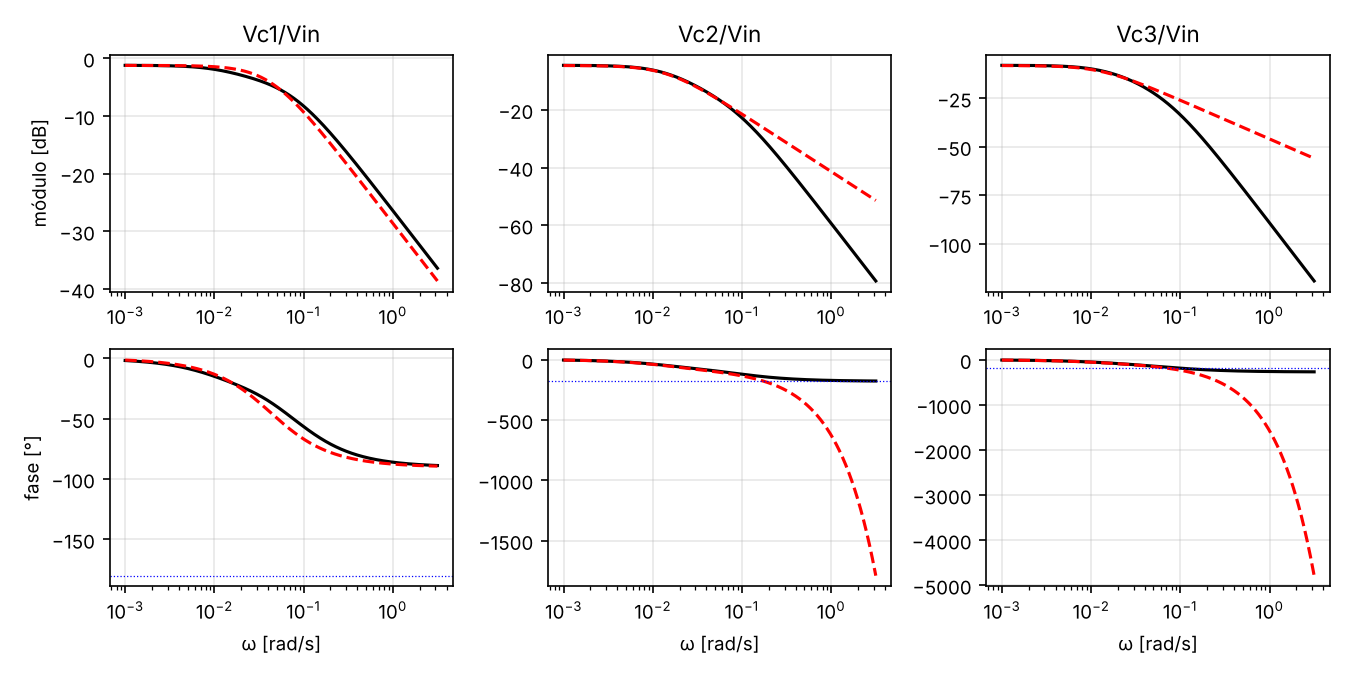
\includegraphics[width=.95\textwidth]{figs/bode.png}
\caption{Bode das FTs completas (preto) e reduzidas (vermelho tracejado).}\end{figure}
Valores em algumas frequências (módulo e fase em graus):
\begin{center}\small
\begin{tabular}{c|cc|cc|cc}\toprule
 & \multicolumn{2}{c|}{$\Vc1$ completa / reduzida} & \multicolumn{2}{c|}{$\Vc2$ completa} & \multicolumn{2}{c}{$\Vc3$ completa / reduzida}\\
$\omega$ [rad/s] & $|G|$ & $\angle G$ & $|G|$ & $\angle G$ & $|G|$ & $\angle G$ / red.\\\midrule
0,01 & 0,8016 (red 0,8445) & $-14{,}8$ ($-13{,}1$) & 0,4888 & $-37{,}7$ & 0,3215 & $-49{,}5$ ($-52{,}8$)\\
0,03 & 0,6503 (0,7106) & $-29{,}6$ ($-35{,}0$) & 0,2622 & $-74{,}9$ & 0,1492 & $-107{,}1$ ($-111{,}4$)\\
0,10 & 0,3854 (0,3419) & $-56{,}5$ ($-66{,}8$) & 0,0726 & $-121{,}3$ & 0,0210 & $-185{,}8$ ($-231{,}2$)\\
0,30 & 0,1550 (0,1228) & $-76{,}9$ ($-81{,}9$) & 0,0113 & $-156{,}7$ & 0,0012 & $-237{,}7$ ($-533{,}1$)\\\bottomrule
\end{tabular}\end{center}

\subsection{Margens de ganho e de fase}
Como $K<1$ em todas as plantas, o módulo da planta sozinha nunca chega a 0 dB: não existe cruzamento de ganho e a margem de fase seria infinita. Para obter margens com significado, fecho a malha com um controlador proporcional $K_c$ e comparo:
\begin{itemize}
\item o \textbf{ganho crítico} $K_{cu}=1/|G(j\omega_{180})|$, onde $\omega_{180}$ é a frequência em que a fase vale $-180^\circ$ (margem de ganho da planta);
\item a \textbf{margem de fase} $PM=180^\circ+\angle\big(K_cG(j\omega_g)\big)$, onde $|K_cG(j\omega_g)|=1$, para $K_c=3,5,10$.
\end{itemize}
\textbf{Cálculo exato de $K_{cu}$ para a FT completa de $\Vc3$ (critério de Routh).}
\begin{formula}Com $K_c$ puro, a equação característica é $1+K_cG(s)=0$. Para um polinômio $a_3s^3+a_2s^2+a_1s+a_0=0$, a linha $s^1$ da tabela de Routh é $\big[a_2a_1-a_3a_0\big]/a_2$; a estabilidade marginal ocorre quando essa linha se anula. O polinômio auxiliar é $a_2s^2+a_0=0$.\end{formula}
Aqui $a_3=11\,416{,}7$, $a_2=1978{,}65$, $a_1=95{,}071$, $a_0=1+K_cK_3$:
\[
a_2a_1=a_3(1+K_{cu}K_3)\ \Rightarrow\ 1+K_{cu}K_3=\frac{a_2a_1}{a_3}=\frac{1978{,}65\cdot95{,}071}{11\,416{,}7}=16{,}477
\]
\[
K_{cu}=\frac{16{,}477-1}{0{,}3971}=38{,}97 .
\]
Frequência de oscilação (polinômio auxiliar): $\omega_u^2=a_0/a_2=(1+K_{cu}K_3)/a_2=a_1/a_3$, logo
\[
\omega_u=\sqrt{\frac{95{,}071}{11\,416{,}7}}=\sqrt{0{,}008328}=0{,}09125\ \mathrm{rad/s},\qquad T_u=\frac{2\pi}{\omega_u}=\frac{6{,}2832}{0{,}09125}=68{,}85\ \mathrm{s}.
\]
\textbf{Para a FT reduzida de $\Vc3$.} Resolvo $-\arctan(\omega\tau)-\omega t_0=-\pi$, isto é, $f(\omega)=\pi-\arctan(78{,}03\omega)-25{,}92\omega=0$, por bisseção (em $f>0$ o ponto fica à esquerda da raiz):
\begin{center}\small
\begin{tabular}{cccc}\toprule passo & intervalo & ponto médio & $f$\\\midrule
1 & [0,010; 0,200] & 0,1050 & $-1{,}029$\\ 2 & [0,010; 0,1050] & 0,0575 & $+0{,}300$\\ 3 & [0,0575; 0,1050] & 0,0813 & $-0{,}379$\\ 4 & [0,0575; 0,0813] & 0,0694 & $-0{,}045$\\ 5 & [0,0575; 0,0694] & 0,0634 & $+0{,}126$\\ 6 & [0,0634; 0,0694] & 0,0664 & $+0{,}040$\\ $\vdots$ & & & \\\bottomrule
\end{tabular}\end{center}
Convergindo: $\omega_{180}=0{,}0678$ rad/s. Verificação: $\arctan(0{,}0678\cdot78{,}03=5{,}290)=79{,}3^\circ=1{,}384$ rad e $\omega t_0=0{,}0678\cdot25{,}92=1{,}757$ rad; soma $=3{,}141$ rad $=\pi$ $\checkmark$. Então
\[
K_{cu}=\frac{\sqrt{1+(\omega_{180}\tau)^2}}{K}=\frac{\sqrt{1+5{,}290^2}}{0{,}3918}=\frac{5{,}383}{0{,}3918}=13{,}74 .
\]
Para $\Vc2$ reduzida o mesmo procedimento dá $\omega_{180}=0{,}176$ rad/s e $K_{cu}=20{,}8$.

\textbf{$\Vc1$ e $\Vc2$ completas.} $\Vc1$ (3 polos, 2 zeros): a fase fica entre $0^\circ$ e $-90^\circ$, nunca chega a $-180^\circ$: $K_{cu}$ não existe. $\Vc2$ (3 polos, 1 zero): a fase tende a $-180^\circ$ por cima sem atingi-la (confirmado no gráfico e por Routh: a linha $s^1$ fica $a_2(a_1+K_cK_2\tau_z)-a_3(1+K_cK_2)>0$ para todo $K_c$, pois $a_2\tau_z>a_3$), também sem $K_{cu}$ finito.

\textbf{Margem de fase, exemplo completo ($\Vc3$ completa, $K_c=5$).} Procuro $\omega_g$ tal que $5|G(j\omega_g)|=1$, isto é, $|G|=0{,}2$. Por tentativa numérica: $\omega_g=0{,}0222$ rad/s. Fase nesse ponto:
\[
-\big[\arctan(0{,}0222\cdot68{,}68)+\arctan(0{,}0222\cdot16{,}00)+\arctan(0{,}0222\cdot10{,}39)\big]=-(56{,}7+19{,}5+13{,}0)=-89{,}3^\circ,
\]
\[
PM=180^\circ-89{,}3^\circ=90{,}7^\circ .
\]
\begin{center}
\begin{tabular}{lcccc}\toprule & & $\Vc1$ & $\Vc2$ & $\Vc3$\\\midrule
\multirow{2}{*}{$K_{cu}$ ($\omega_{180}$ [rad/s])} & completa & $\infty$ & $\infty$ & 39,0 (0,091)\\ & reduzida & $\infty$ & 20,8 (0,176) & 13,7 (0,068)\\\midrule
\multirow{2}{*}{$PM$, $K_c=3$} & completa & $118{,}7^\circ$ & $116{,}4^\circ$ & $134{,}9^\circ$\\ & reduzida & $112{,}6^\circ$ & $113{,}4^\circ$ & $136{,}5^\circ$\\\midrule
\multirow{2}{*}{$PM$, $K_c=5$} & completa & $107{,}0^\circ$ & $93{,}8^\circ$ & $90{,}7^\circ$\\ & reduzida & $103{,}3^\circ$ & $88{,}5^\circ$ & $88{,}6^\circ$\\\midrule
\multirow{2}{*}{$PM$, $K_c=10$} & completa & $98{,}4^\circ$ & $68{,}5^\circ$ & $52{,}1^\circ$\\ & reduzida & $96{,}6^\circ$ & $54{,}8^\circ$ & $32{,}7^\circ$\\\bottomrule
\end{tabular}\end{center}
\begin{just}\textbf{Margem de fase:} praticamente igual para $K_c=3$ e $5$ (diferenças de até $6^\circ$), porque o cruzamento de ganho ocorre em baixa frequência ($<0{,}05$ rad/s), onde a FOPDT reproduz bem a completa. Só com $K_c=10$ o prejuízo é visível ($\Vc3$: $52^\circ$ contra $33^\circ$). \textbf{Margem de ganho:} aqui há prejuízo, e é para o lado \emph{conservador}: o atraso $e^{-t_0s}$ da reduzida faz a fase cair sem limite, enquanto a completa satura em $-180^\circ$ ($\Vc2$) ou $-270^\circ$ ($\Vc3$). Assim a reduzida cruza $-180^\circ$ em frequência menor e prevê $K_{cu}=13{,}7$ contra $39{,}0$ ($\Vc3$): subestima a margem em $\sim$65\,\%. \textbf{Consequência:} sintonizar com a FOPDT é seguro (o ganho fica limitado pelo modelo reduzido), mas na planta real a malha tem mais folga do que a simulação reduzida indica. Já para o método de Ziegler--Nichols (item 4.1) o ganho crítico precisa ser o da planta completa, não o da reduzida.\end{just}

%==================== PARTE 2 ====================
\section{Método de simulação em malha fechada (comum aos itens)}
\subsection{Estrutura do PID (PI\_D paralelo do OpenPLC)}
\begin{formula}
$\displaystyle U(s)=\Big(K_p+\frac{K_i}{s}\Big)\big(R(s)-Y(s)\big)-D(s)\,Y(s),\qquad D(s)=\frac{K_d\,s}{\mu T_d\,s+1},\qquad K_i=\frac{K_p}{T_i},\ K_d=K_pT_d .$
\end{formula}
Aqui $R=SP$, $Y=VP$, $U=SC$ (sinal de controle). \begin{just}A ação proporcional e a integral atuam sobre o erro $e=SP-VP$; a derivada atua \emph{só sobre a VP} (e não sobre o erro) para não derivar os degraus do SP (``chute derivativo''). O filtro de constante $\mu T_d$ ($\mu=0{,}1$) limita o ganho do termo derivativo em alta frequência a $K_p(1+1/\mu)$ (a derivada pura amplificaria o ruído do ADC). É essa a implementação do OpenPLC citada no enunciado.\end{just}
\begin{alerta}\textbf{Nota sobre o programa real do PLC.} O programa \texttt{Prova2.st} usado na bancada \emph{não} tem o filtro $\mu T_d$: a derivada é a de 4 pontos do bloco \texttt{DERIVATIVE} (20 ms), sem filtro. As simulações desta parte (seções 7 a 13) usam o filtro $\mu=0{,}1$ \emph{de projeto}; a análise do efeito dessa diferença está na Seção~\ref{expruido}.\end{alerta}

\subsection{Funções de transferência de malha fechada}
Sendo $Y=GU$ e $PI(s)=K_p+K_i/s$:
\[
U=PI\,R-(PI+D)\,Y=PI\,R-(PI+D)\,G\,U\ \Rightarrow\ U\,[1+(PI+D)G]=PI\,R .
\]
\begin{res}
\[
\frac{U}{R}=\frac{PI}{1+(PI+D)G},\qquad \frac{Y}{R}=\frac{PI\,G}{1+(PI+D)G}.
\]
\end{res}
\textbf{Forma polinomial (para simular).} Escrevo $G=N_G/D_G$, $PI=(K_ps+K_i)/s$ e $D=K_ds/(\mu T_ds+1)$. Levando ao denominador comum $s(\mu T_ds+1)$:
\[\begin{gathered}
PI+D=\frac{(K_ps+K_i)(\mu T_ds+1)+K_ds^2}{s(\mu T_ds+1)}=\frac{C_n}{C_d},\\ C_n=(K_ps+K_i)(\mu T_ds+1)+K_ds^2,\ C_d=s(\mu T_ds+1).
\end{gathered}\]
Substituindo e simplificando (o fator $s$ de $C_d$ cancela com o $s$ do $PI$):
\[
\frac{Y}{R}=\frac{(K_ps+K_i)(\mu T_ds+1)\,N_G}{C_dD_G+C_nN_G},\qquad
\frac{U}{R}=\frac{(K_ps+K_i)(\mu T_ds+1)\,D_G}{C_dD_G+C_nN_G}.
\]
O denominador $C_dD_G+C_nN_G$ é o polinômio característico da malha fechada: seus polos dizem se a malha é estável. Simulo com a rotina \texttt{lsim} (a mesma do script do professor no MATLAB).

\subsection{Planta nas simulações e atraso por Padé}
Uso duas plantas $\Vc3/\Vin$: \textbf{(a) FT reduzida (FOPDT)} (eq.~\eqref{ft3} reduzida: $K=0{,}3918$, $\tau=78{,}03$, $t_0=25{,}92$) e \textbf{(b) FT completa}, eq.~\eqref{ft3}.
\begin{formula}Aproximação de Padé de ordem $n/n$ de $e^{-x}$: $\displaystyle e^{-x}\approx\frac{\sum_{k=0}^{n}(-1)^kc_kx^k}{\sum_{k=0}^{n}c_kx^k}$, $\ c_k=\frac{(2n-k)!\,n!}{(2n)!\,k!\,(n-k)!}$.\end{formula}
\begin{just}O atraso $e^{-t_0s}$ não é uma função racional, e \texttt{lsim} trabalha com polinômios. Com $t_0=25{,}92$ s, o Padé de 1ª ordem (usado no script do professor) distorce bastante; uso a de 3ª ordem ($n=3$).\end{just}
Para $n=3$: $c_0=1$; $c_1=\frac{5!\,3!}{6!\,1!\,2!}=\frac{720}{1440}=\frac12$; $c_2=\frac{4!\,3!}{6!\,2!\,1!}=\frac{144}{1440}=\frac1{10}$; $c_3=\frac{3!\,3!}{6!\,3!\,0!}=\frac{36}{4320}=\frac1{120}$. Com $x=t_0s$ e $t_0=25{,}92$:
\[
e^{-t_0s}\approx\frac{1-\frac{t_0s}{2}+\frac{(t_0s)^2}{10}-\frac{(t_0s)^3}{120}}{1+\frac{t_0s}{2}+\frac{(t_0s)^2}{10}+\frac{(t_0s)^3}{120}}
=\frac{-145{,}12\,s^3+67{,}18\,s^2-12{,}96\,s+1}{145{,}12\,s^3+67{,}18\,s^2+12{,}96\,s+1},
\]
pois $t_0/2=12{,}96$, $t_0^2/10=671{,}8/10=67{,}18$ e $t_0^3/120=17\,414/120=145{,}12$. Para garantir que o Padé não distorce, repeti o item 1.1 com o atraso exato (integração no tempo): diferença máxima na VP de 0,24\,\% da escala.

\subsection{Condições das simulações}
Partida em regime com $SP=SP_0$ e $SC=SP_0/K_{planta}$; em $t=50$ s o SP muda para $SP_1$. As simulações são \textbf{lineares}: não incluem a saturação do SC em 0--100\,\% e só valem enquanto o SC ficar entre esses limites (por isso escolho o degrau de SP de modo que o SC não sature). O valor máximo de $\Vc3$ em regime é $K_3\cdot100=39{,}7\,\%$.

\subsection{Conversão série $\to$ ideal (Eq.\ 5-3.17 do livro)}
\begin{formula}As Tabelas 7-1.1 e 7-4.1 dão o PID na forma real/série:
$\displaystyle C(s)=K_c'\Big(1+\frac1{\tau_I's}\Big)(1+\tau_D's)=K_c'\Big[1+\frac{\tau_D'}{\tau_I'}+\frac1{\tau_I's}+\tau_D's\Big]$,
e o PID ideal/paralelo é $C(s)=K_c\big[1+\frac1{\tau_Is}+\tau_Ds\big]$.\end{formula}
Igualando termo a termo:
\begin{itemize}
\item termo constante: $K_c=K_c'\Big(1+\dfrac{\tau_D'}{\tau_I'}\Big)$;
\item termo em $1/s$: $\dfrac{K_c}{\tau_I}=\dfrac{K_c'}{\tau_I'}\ \Rightarrow\ \tau_I=\tau_I'\,\dfrac{K_c}{K_c'}=\tau_I'\Big(1+\dfrac{\tau_D'}{\tau_I'}\Big)=\tau_I'+\tau_D'$;
\item termo em $s$: $K_c\tau_D=K_c'\tau_D'\ \Rightarrow\ \tau_D=\dfrac{K_c'\tau_D'}{K_c}=\dfrac{\tau_D'}{1+\tau_D'/\tau_I'}=\dfrac{\tau_I'\tau_D'}{\tau_I'+\tau_D'}$.
\end{itemize}
\begin{res}Para o OpenPLC: $K_p=K_c$, $K_i=K_c/\tau_I$, $K_d=K_c\tau_D$.\end{res}

%------------------------------------------------------------------
\section{Item 1.1: PID pela Tabela 7-4.1 (síntese direta)}
\subsection{O que é pedido}
``Uma sintonia de PID segundo o método da tabela 7-4.1 do livro, e verifique o sucesso da sintonia confrontando simulação com o experimental.'' Planta: $\Vc3/\Vin$, FOPDT com $K=0{,}3918$, $\tau=78{,}03$ s, $t_0=25{,}92$ s.

\subsection{De onde vem a tabela (dedução)}
\begin{formula}Síntese direta (Dahlin): escolho a resposta desejada de malha fechada $\dfrac YR=\dfrac{e^{-t_0s}}{\tau_cs+1}$ (1ª ordem com o mesmo atraso da planta) e calculo o controlador que a produz:
\[C(s)=\frac1{G(s)}\,\frac{Y/R}{1-Y/R}.\]\end{formula}
Com $G=\dfrac{Ke^{-t_0s}}{\tau s+1}$, tem-se $1/G=\dfrac{(\tau s+1)e^{t_0s}}{K}$ e
\[
\frac{Y/R}{1-Y/R}=\frac{e^{-t_0s}}{\tau_cs+1-e^{-t_0s}}\ \Rightarrow\ C(s)=\frac{\tau s+1}{K\,(\tau_cs+1-e^{-t_0s})}.
\]
Aproximando o atraso por Padé de 1ª ordem, $e^{-t_0s}\approx\dfrac{1-t_0s/2}{1+t_0s/2}$:
\[
\tau_cs+1-\frac{1-t_0s/2}{1+t_0s/2}=\frac{(\tau_cs+1)(1+\frac{t_0s}2)-(1-\frac{t_0s}2)}{1+\frac{t_0s}2}=\frac{s\big[(\tau_c+t_0)+\frac{\tau_ct_0}{2}s\big]}{1+\frac{t_0s}2},
\]
\[
C(s)=\frac{(\tau s+1)(1+\frac{t_0s}{2})}{K\,s\,\big[(\tau_c+t_0)+\frac{\tau_ct_0}{2}s\big]}
=\underbrace{\frac{\tau}{K(\tau_c+t_0)}}_{K_c'}\Big(1+\frac1{\tau s}\Big)\Big(1+\frac{t_0}{2}s\Big)\frac1{1+\tau_fs},\quad \tau_f=\frac{\tau_ct_0}{2(\tau_c+t_0)} .
\]
Desprezando o filtro $\tau_f$, obtém-se exatamente a linha de PID da Tabela 7-4.1 (forma real/série):
\[
K_c'=\frac{\tau}{K(t_0+\tau_c)},\qquad\tau_I'=\tau,\qquad\tau_D'=\frac{t_0}{2}.
\]
Convertendo para a forma ideal (Seção 7.5) obtém-se a fórmula do script do professor com $\lambda=\tau_c$:
\[
K_c=K_c'\Big(1+\frac{\tau_D'}{\tau_I'}\Big)=\frac{\tau}{K(t_0+\tau_c)}\cdot\frac{2\tau+t_0}{2\tau}=\frac{2\tau+t_0}{2K(\tau_c+t_0)},\quad T_i=\tau+\frac{t_0}2,\quad T_d=\frac{\tau\,t_0/2}{\tau+t_0/2}=\frac{\tau t_0}{2\tau+t_0}.
\]
O único parâmetro de projeto é $\tau_c$ (constante de tempo desejada de malha fechada).

\subsection{Escolha de $\tau_c$}
Testei $\tau_c=20,30,40$ e $60$ s com degrau de SP de 20 para 30\,\% (alcançável, pois o máximo é 39,7\,\%). Resultados (FOPDT / FT completa):
\begin{center}\small
\begin{tabular}{rcccccc}\toprule $\tau_c$ [s] & $K_p$ & $K_i$ & $K_d$ & sobress.\ [\%] & $t_{63,2}$ [s] & pico do SC [\%]\\\midrule
20 & 5,057 & 0,0556 & 56,21 & 2,7 / 2,4 & 51,5 / 54,4 & 114 / 103\\
30 & 4,153 & 0,0456 & 46,16 & 1,5 / 0,6 & 59,0 / 62,0 & 102 / 94\\
\textbf{40} & \textbf{3,523} & \textbf{0,0387} & \textbf{39,15} & 0,7 / 0,0 & 67,9 / 69,6 & 94 / 88\\
60 & 2,703 & 0,0297 & 30,04 & 0,1 / 0,0 & 86,9 / 85,3 & 84 / 80\\\bottomrule
\end{tabular}\end{center}
Em todos os casos $T_i=90{,}99$ s e $T_d=11{,}11$ s (não dependem de $\tau_c$).
\begin{figure}[H]\centering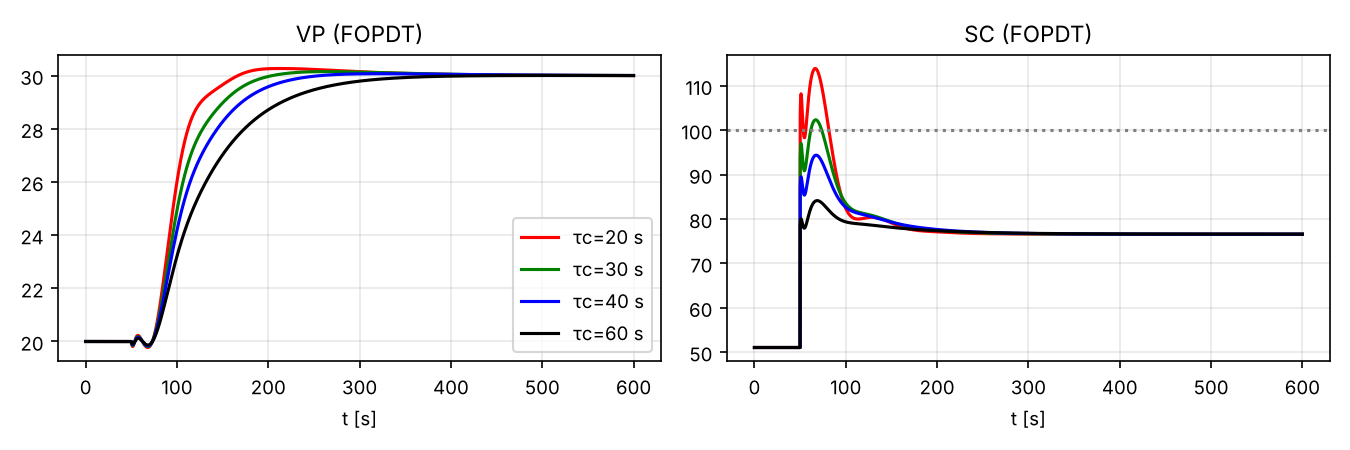
\includegraphics[width=.95\textwidth]{figs/i11_tc.png}\caption{Efeito de $\tau_c$ na VP e no SC (simulação com FOPDT).}\end{figure}
\begin{just}Adoto $\tau_c=40$ s. Com 20 e 30 s o SC da simulação passa de 100\,\% (na bancada o SC saturaria e a simulação linear deixaria de valer). Com 60 s a resposta fica lenta (63,2\,\% em 87 s) sem ganho real. Com 40 s o pico do SC é 94\,\% e o sobressinal é menor que 1\,\%. Além disso $\tau_c=40$ s é maior que o atraso $t_0=25{,}9$ s, o que mantém a malha robusta ao tempo morto. O script do professor usa $\lambda=60$ s (para a planta dele, $\tau=82{,}5$ s); se ele indicar outro valor, basta trocar $\tau_c$ nas fórmulas.\end{just}

\subsection{Cálculo passo a passo ($\tau_c=40$ s)}
\textbf{Passo 1 --- forma real/série (Tabela 7-4.1):}
\[
K_c'=\frac{\tau}{K(t_0+\tau_c)}=\frac{78{,}03}{0{,}3918\,(25{,}92+40)}=\frac{78{,}03}{0{,}3918\cdot65{,}92}=\frac{78{,}03}{25{,}83}=3{,}021\ \%\mathrm{SC}/\%\mathrm{VP},
\]
\[
\tau_I'=\tau=78{,}03\ \mathrm{s},\qquad \tau_D'=\frac{t_0}2=\frac{25{,}92}{2}=12{,}96\ \mathrm{s}.
\]
\textbf{Passo 2 --- conversão para a forma ideal (Seção 7.5):}
\[
K_p=K_c'\Big(1+\frac{\tau_D'}{\tau_I'}\Big)=3{,}021\Big(1+\frac{12{,}96}{78{,}03}\Big)=3{,}021\cdot1{,}1661=3{,}523,
\]
\[
T_i=\tau_I'+\tau_D'=78{,}03+12{,}96=90{,}99\ \mathrm{s},\qquad T_d=\frac{\tau_I'\tau_D'}{\tau_I'+\tau_D'}=\frac{78{,}03\cdot12{,}96}{90{,}99}=\frac{1011{,}2}{90{,}99}=11{,}11\ \mathrm{s}.
\]
\textbf{Conferência com a fórmula direta (script do professor):} $K_p=\dfrac{2\cdot78{,}03+25{,}92}{2\cdot0{,}3918\cdot(40+25{,}92)}=\dfrac{181{,}98}{51{,}66}=3{,}523$ $\checkmark$.

\textbf{Passo 3 --- parâmetros do PI\_D paralelo do OpenPLC:}
\[\begin{gathered}
K_i=\frac{K_p}{T_i}=\frac{3{,}523}{90{,}99}=0{,}03872\ \mathrm{s^{-1}},\\ K_d=K_pT_d=3{,}523\cdot11{,}11=39{,}15\ \mathrm{s},\\ \mu T_d=0{,}1\cdot11{,}11=1{,}11\ \mathrm{s}.
\end{gathered}\]
\begin{res}$K_p=3{,}523$;\quad $K_i=0{,}03872$ (ou $T_i=90{,}99$ s);\quad $K_d=39{,}15$ (ou $T_d=11{,}11$ s);\quad $\mu=0{,}1$.\\
Lei de controle: $SC(t)=K_pe(t)+K_i\!\int e\,dt-K_d\dfrac{d}{dt}VP_{filtrada}(t)$.\end{res}

\subsection{Simulação}
Degrau de SP de 20 para 30\,\% em $t=50$ s, partindo do regime com $SC_0=20/K\approx51{,}0\,\%$ (FOPDT) e $50{,}4\,\%$ (FT completa, $K_3=0{,}3971$). \emph{Comportamento imediato do SC:} em $t=50$ s o termo proporcional dá um salto $K_p\Delta SP=3{,}523\cdot10=35{,}2$ pontos (de 51,0 para $\approx86$\,\%); a derivada não contribui com ``chute'' porque age só sobre a VP.
\begin{figure}[H]\centering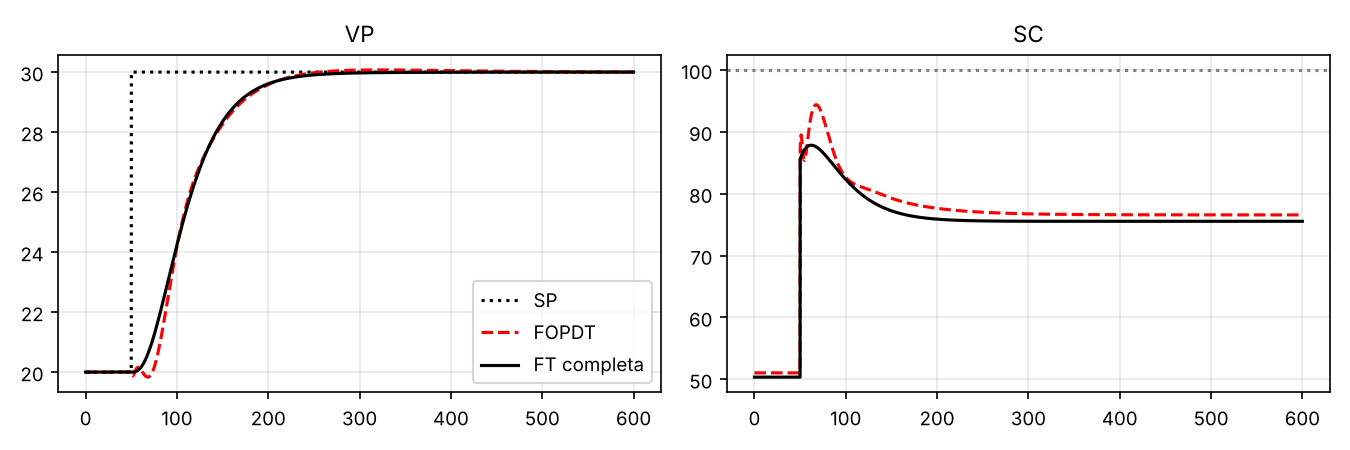
\includegraphics[width=.95\textwidth]{figs/i11.png}\caption{Item 1.1: VP e SC simulados (FOPDT em vermelho tracejado; FT completa em preto).}\end{figure}
\begin{center}\small
\begin{tabular}{lccccc}\toprule & sobress.\ [\%] & $t_{63,2}$ [s] & $t_s$ ($\pm2\%$) [s] & pico do SC [\%] & SC final [\%]\\\midrule
FOPDT & 0,7 & 67,9 & 169,6 & 94,4 & 76,6\\ FT completa & 0,0 & 69,6 & 172,8 & 87,8 & 75,5\\\bottomrule\end{tabular}\end{center}
$SC_{final}=SP_1/K$: $30/0{,}3918=76{,}6$ (FOPDT) e $30/0{,}3971=75{,}5$ (completa); a diferença vem de $K$ ($1{,}3\,\%$).

\textbf{Polos de malha fechada} (raízes de $C_dD_G+C_nN_G$, com Padé de 3ª ordem): FOPDT: $-0{,}511\pm0{,}397j$, $-0{,}0638\pm0{,}0903j$, $-0{,}0182$, $-0{,}0130$; FT completa: $-0{,}902$, $-0{,}0832$, $-0{,}0422$, $-0{,}0351$, $-0{,}0109$. Todos com parte real negativa $\Rightarrow$ malha estável nos dois modelos.

\textbf{Margens da malha aberta $L=(PI+D)G$:} FOPDT: $GM=3{,}7$ (11,4 dB), $PM=78{,}4^\circ$; FT completa: $GM=59{,}7$ (35,5 dB), $PM=81{,}4^\circ$. A margem de fase é praticamente igual nos dois modelos; a margem de ganho da FOPDT é muito menor, como visto na Seção 6.2.
\begin{just}Os dois modelos concordam no formato e na escala de tempo da VP. A FOPDT mostra um pequeno sobressinal e um pico de SC maior (94 contra 88\,\%) porque seu atraso puro e o ganho um pouco diferente alteram a ação proporcional+derivativa.\end{just}
\begin{res}\textbf{Experimento realizado (arquivo \texttt{Q11.csv}).} Procedimento: manual com $SO=50\,\%$ ($VP=19{,}4\,\%$), malha fechada com $SP=VP$ e degrau $19{,}5\to30\,\%$. Resultado: sem sobressinal significativo, erro nulo em regime, salto do SC de $37{,}0$ pontos (previsto $K_p\Delta SP=36{,}9$), VP experimental $\times$ simulada com RMS de $0{,}38\,\%$. O sinal \texttt{SO} apresenta picos por ruído da derivada. Análise completa na Seção~\ref{expdados} e seguintes (Seções~\ref{expdados} a \ref{conclq1}).\end{res}

%------------------------------------------------------------------
\section{Item 2.1: PID 2GL (método do $\alpha$ de Juliana Dalmaso)}\label{it21}
\subsection{O que é pedido}
``Uma sintonia do PID 2GL seguindo a mesma metodologia adotada no TCC de Juliana Dalmaso da Silva para escolha do alfa e verifique o sucesso da sintonia confrontando simulação com o experimental quando é aplicado um degrau no SP.''

\subsection{A metodologia do TCC}
Com PID de 1 grau de liberdade, a malha fechada é $VP=\dfrac{PID\,H}{1+PID\,H}SP+\dfrac{H}{1+PID\,H}D$ ($H$ = planta, $D$ = distúrbio). Uma única sintonia não otimiza as duas respostas: a sintonia \emph{servo} (boa para SP) tem ganho menor e a \emph{regulatória} (boa para distúrbio) tem ganho maior, mas ao mudar o SP exige muito do atuador e satura o SC. O PID 2GL resolve isso colocando um filtro no SP:
\begin{formula}
$\displaystyle C_f(s)=\frac{(1-\alpha)T_is+1}{T_is+1},\qquad VP=\frac{C_f\,PI\,G}{1+(PI+D)G}\,SP+\frac{G}{1+(PI+D)G}\,D .$
\end{formula}
\begin{just}$C_f$ aparece \emph{só} na resposta ao SP; a resposta ao distúrbio fica a da sintonia regulatória, qualquer que seja $\alpha$. O filtro é um avanço--atraso. Para ver o efeito, multiplique $C_f$ pelo $PI=K_p\dfrac{T_is+1}{T_is}$: o zero $(T_is+1)$ do PI cancela o polo de $C_f$ e fica $C_f\,PI=K_p\dfrac{(1-\alpha)T_is+1}{T_is}$. Com $\alpha=0$ é o PI\_D comum; com $\alpha\to1$ vira $K_p/(T_is)$, isto é, o SP entra só pela integral (resposta suave, sem salto proporcional no SC).\end{just}
O TCC tem quatro passos: (1) sintonizar o PID para \textbf{controle regulatório} (síntese direta com $\tau_c$ pequeno); (2) sintonizar um PID para \textbf{controle servo} (mesma síntese com $\tau_c$ grande, no TCC $\tau_c=\tau$) e simulá-lo só como \emph{referência} da resposta desejada ao SP; (3) simular o 2GL variando $\alpha$ (no TCC: 0,4; 0,7; 0,99); (4) escolher o $\alpha$ cuja resposta ao SP fica mais próxima da servo, observando que o SC fique menor que o do regulatório (no TCC o $\alpha=0{,}7$ foi o escolhido).

\subsection{Passos 1 e 2: sintonias regulatória e servo}
Mesma fórmula do item 1.1, mudando $\tau_c$. Servo: $\tau_c=\tau=78{,}03$ s. Regulatório: $\tau_c=20$ s (pequeno, mas não menor que o razoável para $t_0=25{,}9$ s; com FOPDT: $GM=2{,}6$, $PM=73^\circ$).
\begin{align*}
\text{servo:}\ K_c'&=\frac{78{,}03}{0{,}3918\,(25{,}92+78{,}03)}=\frac{78{,}03}{0{,}3918\cdot103{,}95}=\frac{78{,}03}{40{,}73}=1{,}916\\ &\Rightarrow K_p=1{,}916\cdot1{,}1661=2{,}234\\
\text{regulatório:}\ K_c'&=\frac{78{,}03}{0{,}3918\,(25{,}92+20)}=\frac{78{,}03}{0{,}3918\cdot45{,}92}=\frac{78{,}03}{17{,}99}=4{,}337\\ &\Rightarrow K_p=4{,}337\cdot1{,}1661=5{,}057
\end{align*}
Nos dois casos $T_i=90{,}99$ s e $T_d=11{,}11$ s (não dependem de $\tau_c$). Regulatório: $K_i=5{,}057/90{,}99=0{,}05558$, $K_d=5{,}057\cdot11{,}11=56{,}21$. Servo: $K_i=2{,}234/90{,}99=0{,}02455$, $K_d=2{,}234\cdot11{,}11=24{,}83$. Como esperado pelo TCC, \textbf{o ganho do regulatório ($K_p=5{,}06$) é maior que o do servo ($2{,}23$).}

\subsection{Passos 3 e 4: escolha do $\alpha$}
Simulei o 2GL (regulatório + $C_f$) com $\alpha=0{,}4$; $0{,}7$; $0{,}99$ (valores do TCC) e fiz também uma varredura de $\alpha$ de 0 a 0,99 em passos de 0,01, medindo o erro RMS entre a VP do 2GL e a VP servo (referência) em $50<t<550$ s, em \% do degrau:
\[
\varepsilon(\alpha)=\frac{100}{\Delta SP}\sqrt{\frac1N\sum_k\big(VP_{2GL}(t_k;\alpha)-VP_{servo}(t_k)\big)^2},\qquad \Delta SP=10\,\%.
\]
\begin{figure}[H]\centering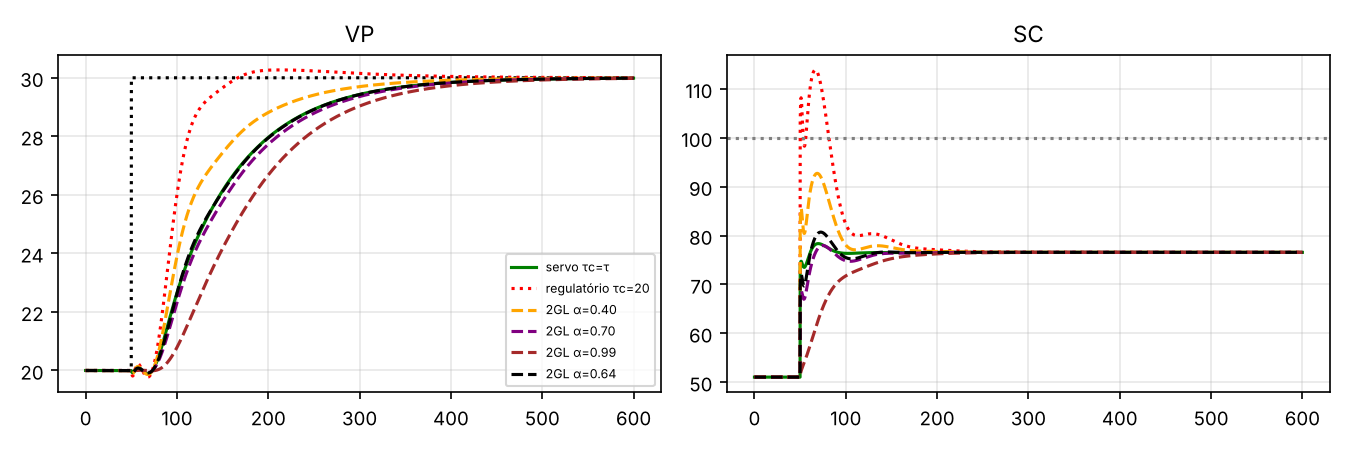
\includegraphics[width=.95\textwidth]{figs/i21.png}\caption{Item 2.1: PI\_D servo (verde), regulatório (vermelho pontilhado) e 2GL para $\alpha=0{,}4$; $0{,}7$; $0{,}99$ e $0{,}64$ (preto). Simulação com FOPDT.}\end{figure}
\begin{figure}[H]\centering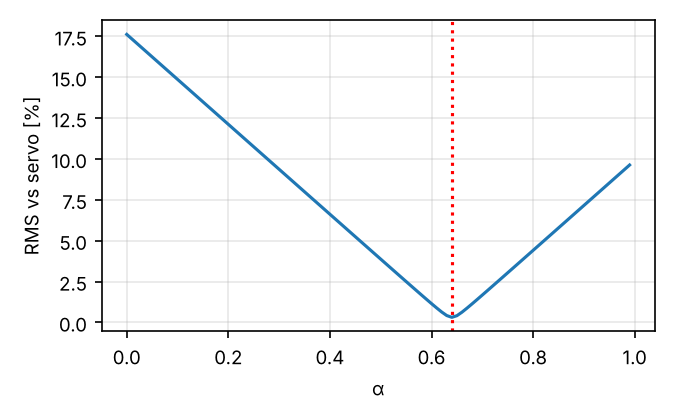
\includegraphics[width=.5\textwidth]{figs/i21_alpha.png}\caption{Erro RMS entre a VP do 2GL e a VP servo em função de $\alpha$.}\end{figure}
\begin{center}\small
\begin{tabular}{lcccc}\toprule Caso (FOPDT) & sobress.\ [\%] & $t_{63,2}$ [s] & pico do SC [\%] & RMS $\times$ servo [\%]\\\midrule
PI\_D servo ($\tau_c=\tau$) & 0,0 & 104 & 78 & (referência)\\
PI\_D regulatório ($\tau_c=20$) & 2,7 & 51,5 & 114 & 17,6\\
2GL $\alpha=0{,}40$ & 0,0 & 74,4 & 92,7 & 6,62\\
2GL $\alpha=0{,}70$ & 0,0 & 111,4 & 78,0 & 1,67\\
2GL $\alpha=0{,}99$ & 0,0 & 141,3 & 76,6 & 9,63\\
\textbf{2GL $\alpha=0{,}64$} & 0,0 & 104,5 & 80,7 & \textbf{0,31}\\\bottomrule\end{tabular}\end{center}
O mínimo ocorre em $\alpha=0{,}64$ com $\varepsilon=0{,}31\,\%$. (Todos os $\alpha$ desta seção são os do TCC/Omron, com $C_f=\frac{(1-\alpha)T_is+1}{T_is+1}$; ao digitar no programa, usar $\mathtt{alfa}=1-\alpha$, Seção~\ref{alfaplc}.)
\begin{just}$\alpha=0{,}4$ ainda é rápido demais (RMS 6,6\,\%) e o SC chega a 93\,\%; $\alpha=0{,}99$ é lento demais (RMS 9,6\,\%, $t_{63}=141$ s). O valor $\alpha=0{,}7$ do TCC dá RMS 1,7\,\% e funciona, mas a varredura mostra que $\alpha=0{,}64$ reproduz ainda melhor a resposta servo (RMS 0,31\,\%), porque o $\alpha$ ótimo depende da planta (aqui, FOPDT com atraso; no TCC era um processo de 1ª ordem sem atraso). Adoto $\alpha=0{,}64$, mantendo a mesma metodologia do TCC (escolha por simulação do $\alpha$ que aproxima o servo, com SC menor que o do regulatório: pico de 81\,\% contra 114\,\%, que satura).\end{just}
Com a FT completa: $t_{63}=102{,}6$ s e pico do SC de 75,5\,\%.

\subsection{Parâmetros finais para o OpenPLC (PI\_D2GL)}
\begin{res}$K_p=5{,}057$;\quad $K_i=0{,}05558\ \mathrm{s^{-1}}$ ($T_i=90{,}99$ s);\quad $K_d=56{,}21$ ($T_d=11{,}11$ s);\quad $\alpha_{TCC}=0{,}64$ (filtro do SP com $\beta=1$ fixo, como no CLP Omron do TCC).\\
\textbf{No programa \texttt{Prova2.st}:} \texttt{kp := 5.057}, \texttt{ki := 0.05558}, \texttt{kd := 56.21} e \textbf{\texttt{alfa := 0.36}}. O programa pondera o SP no termo proporcional com peso $b=\mathtt{alfa}$, que é equivalente ao filtro do TCC com $\mathtt{alfa}=1-\alpha_{TCC}$ (dedução na Seção~\ref{alfaplc}); $\mathtt{alfa}=1$ é o PI\_D comum.\end{res}
\begin{todo}Passar a automático com $SP=VP$ e os parâmetros acima, com \texttt{alfa := 0.36} (\textbf{não 0,64}); aplicar degrau de SP 20 $\to$ 30\,\%; gravar SO, SP, VP. Confrontar VP e SC com a simulação (FOPDT e FT completa). Se possível repetir com \texttt{alfa := 1.0} (PI\_D regulatório comum) para mostrar o efeito de $\alpha$ (SC chegando a 114\,\%, isto é, saturando). Resultados: \underline{\hspace{6cm}}\end{todo}

%------------------------------------------------------------------
\section{Item 3.1: integral do erro mínimo (seção 7-2.3)}\label{it31}
\subsection{O método}
Na seção 7-2.3 o livro apresenta correlações que minimizam um índice de integral do erro, aqui $\mathrm{IAE}=\int_0^\infty|e|\,dt$, para plantas FOPDT. Para o PID ideal, com $r=t_0/\tau$ (válido para $0{,}1<r<1$):
\begin{formula}
\textbf{Tabela 7-2.3 (ponto fixo, Rovira):}\quad $K_c=\dfrac{1{,}086}{K}\,r^{-0{,}869},\quad \tau_I=\dfrac{\tau}{0{,}740-0{,}130\,r},\quad \tau_D=0{,}348\,\tau\,r^{0{,}914}$.\\[3pt]
\textbf{Tabela 7-2.2 (distúrbio, López):}\quad $K_c=\dfrac{1{,}435}{K}\,r^{-0{,}921},\quad \tau_I=\dfrac{\tau}{0{,}878}\,r^{0{,}749},\quad \tau_D=0{,}482\,\tau\,r^{1{,}137}$.
\end{formula}
\begin{just}Como o experimento é um degrau no SP (como nos outros itens), a sintonia principal é a da Tabela 7-2.3 (ponto fixo); calculo também a de distúrbio para comparar. Aqui $r=25{,}92/78{,}03=0{,}3322$, dentro da faixa de validade. As tabelas já fornecem o PID na forma ideal (paralela), então \textbf{não há conversão série$\to$ideal}: $K_p=K_c$, $K_i=K_c/\tau_I$, $K_d=K_c\tau_D$.\end{just}

\subsection{Cálculo passo a passo}
Potências calculadas por logaritmo: $\ln r=\ln0{,}3322=-1{,}1021$.

\textbf{Ponto fixo (Tabela 7-2.3):}
\begin{align*}
r^{-0{,}869}&=e^{-0{,}869\cdot(-1{,}1021)}=e^{0{,}9577}=2{,}606\\
\frac{1{,}086}{K}&=\frac{1{,}086}{0{,}3918}=2{,}772\\
K_p&=2{,}772\cdot2{,}606=\mathbf{7{,}222}\\
T_i&=\frac{78{,}03}{0{,}740-0{,}130\cdot0{,}3322}=\frac{78{,}03}{0{,}740-0{,}0432}=\frac{78{,}03}{0{,}6968}=\mathbf{111{,}98\ s}\\
r^{0{,}914}&=e^{0{,}914\cdot(-1{,}1021)}=e^{-1{,}0073}=0{,}3652\\T_d&=0{,}348\cdot78{,}03\cdot0{,}3652=27{,}15\cdot0{,}3652=\mathbf{9{,}92\ s}\\
K_i&=\frac{K_p}{T_i}=\frac{7{,}222}{111{,}98}=\mathbf{0{,}06449}\\K_d&=K_pT_d=7{,}222\cdot9{,}917=\mathbf{71{,}63}
\end{align*}
\textbf{Distúrbio (Tabela 7-2.2), para comparar:}
\begin{align*}
r^{-0{,}921}&=e^{1{,}0150}=2{,}759\\K_p&=\frac{1{,}435}{0{,}3918}\cdot2{,}759=3{,}663\cdot2{,}759=10{,}11\\
r^{0{,}749}&=e^{-0{,}8254}=0{,}4380\\T_i&=\frac{78{,}03}{0{,}878}\cdot0{,}4380=38{,}93\ \mathrm{s}\\
r^{1{,}137}&=e^{-1{,}2531}=0{,}2856\\T_d&=0{,}482\cdot78{,}03\cdot0{,}2856=10{,}74\ \mathrm{s}\\
K_i&=10{,}11/38{,}93=0{,}2596\\K_d&=10{,}11\cdot10{,}74=108{,}6
\end{align*}
\begin{res}Ponto fixo: $K_p=7{,}222$; $K_i=0{,}06449$ ($T_i=111{,}98$ s); $K_d=71{,}63$ ($T_d=9{,}92$ s); $\mu=0{,}1$.\end{res}

\subsection{Simulação}
Degrau de SP de 20 para 25\,\% em $t=50$ s (menor que nos outros itens porque o ganho alto desta sintonia faria o SC passar de 100\,\% com 20 $\to$ 30\,\%).
\begin{figure}[H]\centering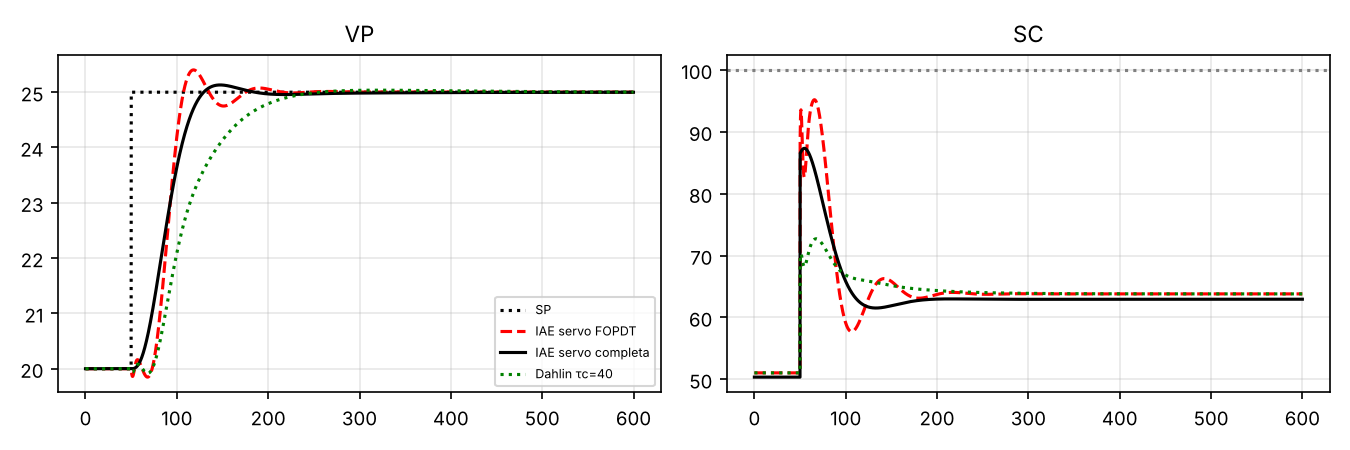
\includegraphics[width=.95\textwidth]{figs/i31.png}\caption{Item 3.1: IAE ponto fixo (FOPDT tracejado vermelho; FT completa preto) e Dahlin $\tau_c=40$ s do item 1.1 (verde pontilhado), degrau 20 $\to$ 25\,\%.}\end{figure}
\begin{center}\small
\begin{tabular}{lcccc}\toprule Sintonia (20 $\to$ 25\,\%), FOPDT / completa & sobress.\ [\%] & $t_{63,2}$ [s] & $t_s$ [s] & pico do SC [\%]\\\midrule
IAE ponto fixo (7-2.3) & 8,1 / 2,6 & 43,7 / 44,4 & 117 / 110 & 95 / 87\\
IAE distúrbio (7-2.2) & 83,6 / 42,3 & 37,8 / 33,3 & 227 / 201 & 129 / 107\\
Dahlin $\tau_c=40$ s (item 1.1) & 0,7 / 0,0 & 67,9 / 69,6 & 170 / 173 & 73 / 69\\\bottomrule\end{tabular}\end{center}
Margens da malha aberta com a sintonia de ponto fixo: FOPDT $GM=1{,}9$, $PM=64^\circ$; FT completa $GM=32{,}0$, $PM=71^\circ$.
\begin{just}A sintonia de ponto fixo é a mais rápida ($t_{63}=44$ s contra 68 s do Dahlin), à custa de sobressinal maior (8,1\,\% na FOPDT, 2,6\,\% na completa) e de $K_p$ mais alto --- esperado de um método que minimiza o erro integral sem penalizar o esforço de controle. A sintonia de distúrbio é ainda mais agressiva e, aplicada a um degrau de SP, produz sobressinal de 84\,\% na FOPDT: foi projetada para rejeitar distúrbios, não para seguir SP (a ideia do TCC: servo e regulatório exigem sintonias diferentes). A diferença de sobressinal entre FOPDT e completa vem do atraso puro da FOPDT, que reduz a margem de ganho (1,9 contra 32).\end{just}
\begin{todo}\textbf{Roteiro completo, previsão e planilha: Seção~\ref{q31exp}.} Mesmo procedimento do item 1.1 com $K_p=7{,}222$, $K_i=0{,}06449$, $K_d=71{,}63$, $\mu=0{,}1$ e degrau de SP 20 $\to$ 25\,\%. Confrontar VP e SC com a figura. Resultados: \underline{\hspace{6cm}}\end{todo}

%------------------------------------------------------------------
\section{Item 4.1: Ziegler--Nichols de razão de decaimento 1/4 (Tabela 7-1.1)}\label{it41}
\subsection{O método}
A Tabela 7-1.1 usa o \textbf{ganho final} $K_{cu}$ e o \textbf{período final} $T_u$: com controle só proporcional, aumenta-se $K_c$ até a VP oscilar com amplitude constante; $K_{cu}$ é esse ganho e $T_u$ o período da oscilação. Para o PID (forma real/série), razão de decaimento 1/4 (cada pico é 1/4 do anterior):
\begin{formula}$K_c'=\dfrac{K_{cu}}{1{,}7},\qquad\tau_I'=\dfrac{T_u}{2},\qquad\tau_D'=\dfrac{T_u}{8}$, convertidos à forma ideal pela Seção 7.5.\end{formula}
\subsection{$K_{cu}$ e $T_u$}
Experimentalmente serão medidos na bancada (teste de ganho final). Para poder simular, calculo-os da FT completa de $\Vc3$ pelo critério de Routh (Seção 6.2): $K_{cu}=38{,}97$, $\omega_u=0{,}09125$ rad/s, $T_u=68{,}85$ s. Confirmação pelos polos de $1+K_cG(s)=0$:
\begin{center}\small\begin{tabular}{ccc}\toprule $K_c$ & polos complexos dominantes & comportamento\\\midrule
$0{,}5K_{cu}=19{,}5$ & $-0{,}0108\pm0{,}0702j$ & oscilação amortece\\
$K_{cu}=39{,}0$ & $\approx0\pm0{,}0913j$ & oscilação sustentada, $T_u=2\pi/0{,}0913=68{,}85$ s\\
$1{,}2K_{cu}=46{,}8$ & $+0{,}0033\pm0{,}0975j$ & oscilação cresce (instável)\\\bottomrule\end{tabular}\end{center}
\begin{figure}[H]\centering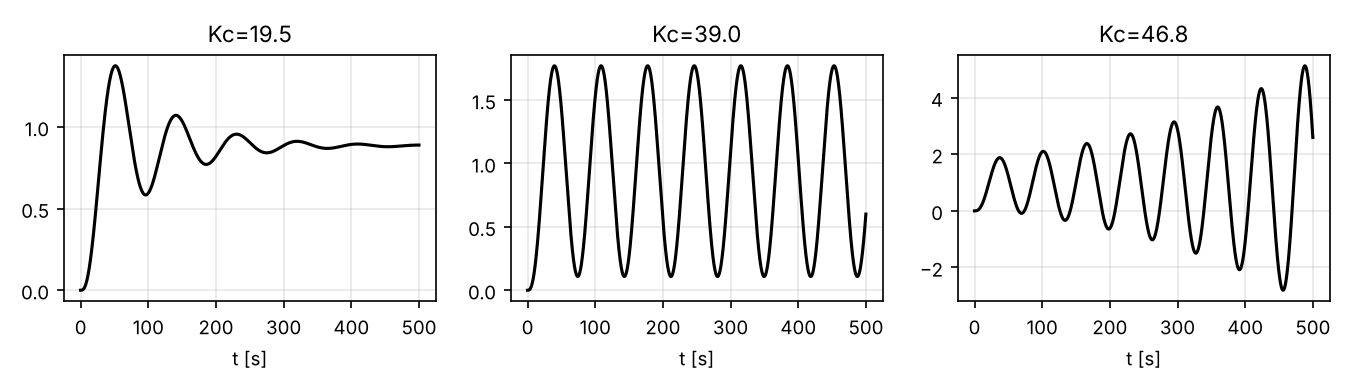
\includegraphics[width=.95\textwidth]{figs/i41_kcu.png}\caption{Teste de ganho final simulado (FT completa, $K_c$ puro, degrau no SP).}\end{figure}
\begin{just}Uso a FT \emph{completa} (e não a reduzida) para obter $K_{cu}$ e $T_u$ porque o método de Ziegler--Nichols exige o comportamento real da planta no limite de estabilidade. A FOPDT daria $K_{cu}=13{,}7$ e $T_u=92{,}7$ s, bem diferentes do real (39,0 e 68,9 s). Na bancada a oscilação sustentada será limitada pela saturação do SC em 0--100\,\%; deve-se registrar o menor $K_c$ que sustenta a oscilação e o período $T_u$ medido, e recalcular os parâmetros com as mesmas fórmulas abaixo.\end{just}

\subsection{Cálculo passo a passo}
\textbf{Passo 1 --- forma real/série:}
\[
K_c'=\frac{K_{cu}}{1{,}7}=\frac{38{,}97}{1{,}7}=22{,}92,\qquad\tau_I'=\frac{T_u}2=\frac{68{,}85}{2}=34{,}43\ \mathrm{s},\qquad\tau_D'=\frac{T_u}8=\frac{68{,}85}{8}=8{,}607\ \mathrm{s}.
\]
\textbf{Passo 2 --- forma ideal (Seção 7.5):}
\[
K_p=K_c'\Big(1+\frac{\tau_D'}{\tau_I'}\Big)=22{,}92\Big(1+\frac{8{,}607}{34{,}43}\Big)=22{,}92\cdot1{,}25=28{,}65,
\]
\[
T_i=\tau_I'+\tau_D'=34{,}43+8{,}607=43{,}03\ \mathrm{s},\qquad T_d=\frac{34{,}43\cdot8{,}607}{43{,}03}=\frac{296{,}3}{43{,}03}=6{,}885\ \mathrm{s}.
\]
\emph{Conferência por fórmula direta:} como $\tau_D'/\tau_I'=1/4$ sempre, $K_p=1{,}25\,K_{cu}/1{,}7=0{,}735K_{cu}=28{,}65$, $T_i=\frac58T_u=43{,}03$ s e $T_d=\frac1{10}T_u=6{,}885$ s $\checkmark$.

\textbf{Passo 3 --- OpenPLC:}
\[
K_i=\frac{K_p}{T_i}=\frac{28{,}65}{43{,}03}=0{,}6659\ \mathrm{s^{-1}},\qquad K_d=K_pT_d=28{,}65\cdot6{,}885=197{,}3\ \mathrm{s},\qquad\mu=0{,}1 .
\]
O ganho em alta frequência do PID (com o filtro $\mu=0{,}1$) é $K_p(1+1/\mu)=28{,}65\cdot11\approx315$: controlador de ganho alto, sensível a ruído de medição (a quantização do ADC é 0,098\,\%).
\begin{res}$K_p=28{,}65$;\ $K_i=0{,}6659$ ($T_i=43{,}03$ s);\ $K_d=197{,}3$ ($T_d=6{,}885$ s);\ $\mu=0{,}1$.\end{res}

\subsection{Simulação}
Degrau de SP de 10 para 12\,\% em $t=50$ s (pequeno porque o ganho alto faria o SC saturar em degraus maiores); $SC_0=10/0{,}3971=25{,}2\,\%$.
\begin{figure}[H]\centering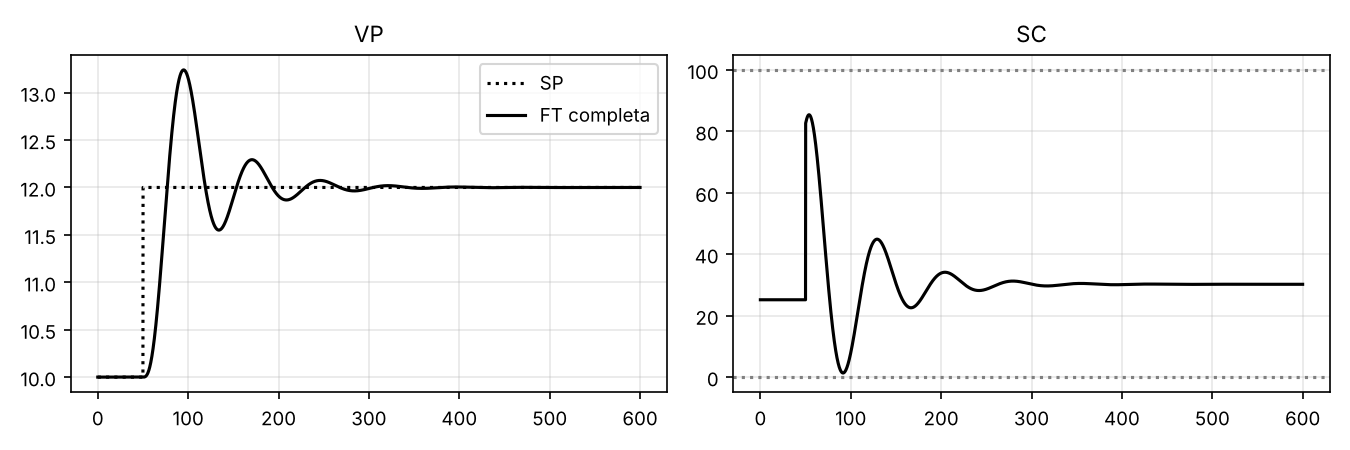
\includegraphics[width=.95\textwidth]{figs/i41.png}\caption{Item 4.1: PID de Ziegler--Nichols simulado com a FT completa.}\end{figure}
\begin{center}\small\begin{tabular}{lccccc}\toprule & sobress.\ [\%] & $t_{63,2}$ [s] & $t_s$ [s] & pico do SC [\%] & $GM$ / $PM$\\\midrule FT completa & 62 & 21 & 209 & 85 & 7,8 / 22$^\circ$\\\bottomrule\end{tabular}\end{center}
\textbf{Razão de decaimento.} Na simulação o 1º excesso acima do SP final é $1{,}24\,\%$ e o 2º é $0{,}29\,\%$ (instantes 95 s e 171 s): razão $=0{,}293/1{,}24=0{,}236\approx1/4$, que é o critério de projeto do método.

\textbf{Por que não simular com a FOPDT.} Os polos de malha fechada da FOPDT com esta sintonia têm parte real positiva ($+0{,}027\pm0{,}087j$ s$^{-1}$): a malha é \emph{instável}, porque $K_c'=22{,}9$ e $K_p=28{,}7$ são maiores que o ganho final da FOPDT ($K_{cu,red}=13{,}7$). Com a FT completa, todos os polos de malha fechada têm parte real negativa (o maior é $-0{,}0176$).
\begin{figure}[H]\centering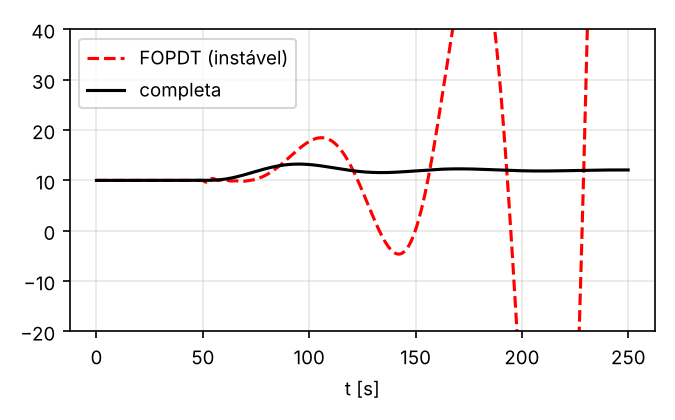
\includegraphics[width=.5\textwidth]{figs/i41_unst.png}\caption{O mesmo PID aplicado à FOPDT (instável) e à FT completa.}\end{figure}
\begin{just}A sintonia de Z--N foi \emph{projetada} para uma planta real em que se mediu $K_{cu}$ e $T_u$; o modelo FOPDT, ao trocar 3 polos por 1 polo e atraso, tem margem de ganho menor, então a sintonia que é estável na planta completa torna a FOPDT instável. Os parâmetros de Z--N só são válidos com $K_{cu}$ e $T_u$ da planta real. A resposta tem sobressinal grande (62\,\% do degrau), característico da razão 1/4; o SC chega a tocar o limite inferior no primeiro retorno, o que na bancada produzirá saturação e leve diferença em relação à simulação linear.\end{just}
\begin{todo}\textbf{Roteiro completo, previsão e planilha: Seção~\ref{q41exp} (e I\_PD na Seção~\ref{q42exp}).} (i) Teste de ganho final: apenas $K_p$ ($K_i=K_d=0$), aumentar até oscilação sustentada, anotar $K_{cu}$ e $T_u$ (esperado: Figura do teste acima); (ii) recalcular os parâmetros com as fórmulas acima e implementar $K_p$, $K_i$, $K_d$, $\mu=0{,}1$; (iii) degrau de SP 10 $\to$ 12\,\%, gravar SO, SP, VP; (iv) confrontar VP e SC com a figura de simulação acima. Resultados: \underline{\hspace{6cm}}\end{todo}

%------------------------------------------------------------------
\section{Resumo dos controladores (para o OpenPLC)}
\begin{center}\small
\begin{tabular}{lccccc}\toprule Sintonia & $K_p$ & $T_i$ [s] & $T_d$ [s] & $K_i=K_p/T_i$ & $K_d=K_pT_d$\\\midrule
1.1 Dahlin ($\tau_c=40$ s) & 3,523 & 90,99 & 11,11 & 0,03872 & 39,15\\
2.1 PI\_D2GL (regulatório $\tau_c=20$ s; $\alpha_{TCC}=0{,}64$ $\Rightarrow$ \texttt{alfa}$=0{,}36$ no programa) & 5,057 & 90,99 & 11,11 & 0,05558 & 56,21\\
3.1 IAE ponto fixo (7-2.3) & 7,222 & 111,98 & 9,92 & 0,06449 & 71,63\\
4.1 Ziegler--Nichols (7-1.1) & 28,65 & 43,03 & 6,885 & 0,6659 & 197,3\\\bottomrule\end{tabular}\end{center}
Derivada na VP; $T_i$ e $T_d$ em segundos e $K_p$ em \%SC/\%VP. Nos projetos usei $\mu=0{,}1$, mas \textbf{o programa real não tem esse filtro} (Seção~\ref{secst}). A coluna $\alpha$ da tabela é o $\alpha$ do TCC; no programa, \texttt{alfa}$=1-\alpha$ ($0{,}36$ para o item 2.1; \texttt{alfa}$=0$ para o I\_PD do item 4.2).

\section{Conclusões}
\begin{itemize}
\item As FTs completas, deduzidas das equações dos nós com os $R$ e $C$ medidos, têm três polos reais ($\tau=68{,}7$; $16{,}0$; $10{,}4$ s) e reproduzem o degrau experimental com RMS de 0,7--1,7\,\% do degrau.
\item $\Vc1$ é curva tipo C ($\tau=23{,}3$ s, sem atraso); $\Vc2$ e $\Vc3$ são tipo S (Smith: $\Vc3$: $K=0{,}392$, $\tau=78{,}0$ s, $t_0=25{,}9$ s).
\item A FOPDT mantém a margem de fase da malha aberta (diferenças de até $6^\circ$ para $K_c\le5$) e subestima a margem de ganho (é conservadora). Por isso as sintonias dos itens 1.1, 2.1 e 3.1 são calculadas com a FOPDT (como pede o enunciado), enquanto $K_{cu}$ e $T_u$ do item 4.1 devem vir da planta real.
\item Os quatro controladores foram simulados (VP e SC, FOPDT e FT completa). Os ensaios da Questão 1 (itens 1.1, 1.2 e 1.3) já foram realizados e analisados nas Seções~\ref{expdados} a \ref{conclq1}; as comparações experimentais dos itens 2.1, 2.2, 3.1, 4.1 e 4.2 ficam para os ensaios correspondentes.
\end{itemize}

%==================== PARTE 3: RESULTADOS EXPERIMENTAIS (QUESTÃO 1) ====================
\section{Resultados experimentais da Questão 1: dados e método de análise}\label{expdados}
Nesta parte confronto os ensaios feitos na bancada (OpenPLC + Arduino + ScadaBR) com a simulação teórica das seções anteriores. Foram realizados quatro registros:
\begin{center}\small
\begin{tabular}{llp{8.2cm}}\toprule Arquivo & Item & O que foi feito\\\midrule
\texttt{Q11.csv} & 1.1 & Malha fechada com a sintonia de Dahlin; degrau de SP $19{,}5\to30\,\%$\\
\texttt{Q12.csv} & 1.2 & Transferência manual$\to$automático \emph{sem} VP-tracking (SP diferente da VP)\\
\texttt{Q13a.csv} & 1.3 & SP inalcançável (55\,\%) e retorno a 20\,\%, \emph{sem} anti reset windup\\
\texttt{Q13b.csv} & 1.3 & Mesma sequência, \emph{com} anti reset windup\\\bottomrule\end{tabular}\end{center}

\subsection{Formato dos arquivos e tratamento}
O ScadaBR grava um arquivo CSV em formato ``longo'': cada linha traz o \emph{nome do ponto} (\texttt{uno - SO}, \texttt{SP}, \texttt{VP}, \texttt{VP1}, \texttt{VP2}), o instante (data e hora, resolução de 1 s) e o valor. Os pontos são $SO=SC$ (sinal de controle), $SP$, $VP=\Vc3$, $VP1=\Vc2$ e $VP2=\Vc1$, todos em \% da escala (100\,\% $=5$ V). Como o número de linhas é diferente em cada variável (por exemplo, em \texttt{Q11.csv}: 2024 para SO e SP, 2028 para VP, 2020 para VP1, 2016 para VP2), \textbf{não se pode dividir o arquivo em 5 partes iguais} (como faz o script de exemplo do professor para arquivos com contagens idênticas). O código desta entrega separa as variáveis pelo \emph{nome}, coloca todas numa grade de 1 s e repete o último valor nos instantes sem registro (o código completo está no Apêndice~\ref{apcodigos}).
\begin{just}Os instantes são usados relativos a um evento (início da malha fechada, degrau de SP etc.). A diferença de horário entre o relatório em PDF do ScadaBR e o CSV é só de fuso/formatação e não afeta a análise.\end{just}

\subsection{Premissas}
\begin{enumerate}
\item \textbf{Sintonia usada nos quatro ensaios:} a de Dahlin do item 1.1 ($K_p=3{,}523$; $T_i=90{,}99$ s; $T_d=11{,}11$ s; $\mu=0{,}1$). Os números dos parâmetros digitados não estão nos arquivos; a evidência de que são esses vem do próprio dado: no degrau de SP da Q11, o SO saltou de $49{,}5$ para $86{,}5$\,\% (+$37{,}0$ pontos) para um degrau de SP de $10{,}48$ pontos, o que dá $K_p=37{,}0/10{,}48=3{,}53$, igual ao previsto $3{,}523$. \textbf{Confirme}, na sua anotação do ensaio, se os valores digitados foram esses.
\item \textbf{Limites do SC:} em todos os quatro arquivos o SO nunca saiu da faixa $[9{,}99;\,99{,}94]\,\%$ (o mínimo $9{,}99485$ e o máximo $99{,}940875=100\cdot1023/1024$ se repetem em todos). Ou seja, o sinal de controle está limitado, na prática, a \textbf{$\approx10\,\%$ (e não 0\,\%) até $\approx99{,}94\,\%$}. Nas simulações aplico esses mesmos limites.
\item \textbf{Modelo da planta:} FT completa das seções 2 e 3 (com os $R$ e $C$ medidos), mais um deslocamento (\emph{offset}) de saída obtido do ajuste da Seção~\ref{expplanta}.
\end{enumerate}
\subsection{O simulador de comparação}
Simulo a malha fechada em tempo discreto (passo 0,05 s) com a planta de 3ª ordem completa:
\[
x[k+1]=\Phi\,x[k]+\Gamma\,u[k],\quad \Phi=e^{A\,\Delta t},\ \Gamma=A^{-1}(\Phi-I)B,\qquad VP=x_3+\text{offset},
\]
com $A$ e $B$ da Seção 2 (espaço de estados da Lista 2). O controlador é o PI\_D do OpenPLC: $u=K_pe+I-D_{filtr}(VP)$, com $I[k+1]=I[k]+K_ie\,\Delta t$, derivada sobre a VP com filtro de constante $\mu T_d$, saturação em $[10;\,99{,}94]$ e anti-windup por \emph{clamping} (para de integrar quando $u$ está saturado e o erro empurra mais para a saturação). Na partida, o estado do circuito é o de regime correspondente ao $SO$ manual e a integral recebe o valor desse $SO$ (transferência sem solavanco, que é o que o bloco faz quando $SP=VP$).
\begin{formula}Métricas usadas: erro RMS e erro máximo entre VP experimental e VP simulada, $\varepsilon_{rms}=\sqrt{\frac1N\sum_k(VP_{sim,k}-VP_{exp,k})^2}$, $\varepsilon_{max}=\max_k|VP_{sim,k}-VP_{exp,k}|$ (em \% da escala). Para o SC uso a \emph{mediana móvel} do SO (explicado na Seção~\ref{expruido}).\end{formula}

%------------------------------------------------------------------
\section{Validação do modelo da planta com os dados do dia}\label{expplanta}
Antes de avaliar o controlador, confirmo que o modelo representa o circuito \emph{nos dias do experimento}.

\textbf{Ganho estático.} Nos patamares de regime em malha aberta (SO constante), obtive os pares:
\begin{center}\small
\begin{tabular}{ccc}\toprule SO [\%] & VP [\%] ($\Vc3$) & $VP/SO$\\\midrule
10,37 & 3,81 e 3,92 & 0,367 e 0,378\\ 20,00 & 7,70 & 0,385\\ 50,00 & 19,43 & 0,389\\ 99,94 & 39,39 & 0,394\\\bottomrule\end{tabular}\end{center}
A razão $VP/SO$ cresce com o SO, então não é um simples ganho proporcional: há um \emph{deslocamento}. A regressão linear dá
\[
VP=0{,}3963\,SO-0{,}262,
\]
isto é, \textbf{inclinação $0{,}3963$ (teórico: $K_3=0{,}3971$, diferença de 0,2\,\%)} e um offset de $-0{,}26$ ponto percentual. O offset é compatível com o ADC/saída do Arduino; a inclinação concorda com a teoria. Para os outros nós: com SO=99,94\,\% medi $VP1=58{,}85$ e $VP2=86{,}70$, que dão $K_2\approx0{,}589$ (teórico 0,591) e $K_1\approx0{,}868$ (teórico 0,869).
\begin{just}O $K=0{,}3918$ da identificação da 1ª parte veio de outro arquivo (outra data e montagem); a diferença para $0{,}3963$ (1,2\,\%) está dentro das tolerâncias de $R$ e $C$ e das condições do dia. Para as simulações desta parte uso a inclinação e o offset do próprio dia dos ensaios.\end{just}

\textbf{Dinâmica.} Para testar a dinâmica sem depender do controlador, excitei o modelo com o \textbf{SO medido} (o que realmente foi aplicado, amostrado a 1 s) e comparei a VP resultante com a VP medida:
\begin{center}\small
\begin{tabular}{lcc}\toprule Registro & RMS [\%] & erro máx.\ [\%]\\\midrule
Q11 (t=1160--2191) & 0,50 & 1,56\\ Q12 (t=20--1075) & 0,20 & 0,65\\ Q13a (t=20--2100) & 0,81 & 4,13\\ Q13b (t=20--825) & 0,50 & 0,97\\\bottomrule\end{tabular}\end{center}
No degrau manual $10{,}37\to50\,\%$ da Q11, o modelo reproduz VP, VP1 e VP2 com RMS de 0,28; 0,56 e 0,66\,\%. \textbf{O modelo físico está validado}: qualquer diferença entre simulação e experimento nas seções seguintes vem do controlador/implementação (ruído, limites, anti-windup), não da planta.

%------------------------------------------------------------------
\section{Item 1.1 experimental (Q11): Dahlin com $\tau_c=40$ s}
\subsection{O que foi feito (linha do tempo extraída do arquivo)}
\begin{enumerate}
\item Manual com $SO=65{,}9\to10{,}4\to50{,}0\,\%$ (a malha fica em aberto; o SP \emph{acompanha a VP} enquanto está em manual, isto é, o bloco tem VP-tracking). Com $SO=50\,\%$ a VP estabiliza em $19{,}4\,\%$.
\item Em $t=1606$ s a malha é fechada com $SP=19{,}5\approx VP$: o SO continua em $\approx50\,\%$ (mediana $49{,}6\,\%$), isto é, \textbf{a transferência é suave} (sem VP-tracking haveria um salto; ver Q12).
\item Em $t=1654$ s: degrau de SP $19{,}52\to30{,}0\,\%$ ($\Delta SP=10{,}48$).
\end{enumerate}
\subsection{Resposta imediata do SC: confirma $K_p$}
No instante do degrau, o SO foi de $49{,}5$ para $86{,}5\,\%$:
\[
\Delta SC_{0^+}=K_p\,\Delta SP=3{,}523\cdot10{,}48=36{,}9\ \text{pontos (previsto)}\qquad\text{medido: }86{,}5-49{,}5=37{,}0\ \text{pontos.}
\]
Esse salto vem só da ação proporcional: a derivada age sobre a VP (e não sobre o erro) e a integral ainda não acumulou. Nos 4 s seguintes o SO sobe $\approx0{,}34$ ponto/s ($86{,}5\to86{,}9\to87{,}3\to87{,}6\to87{,}9$), em boa concordância com a taxa integral $K_ie=0{,}03872\cdot10{,}4=0{,}40$ ponto/s, descontado o efeito da derivada (a VP está começando a subir). Assim, \textbf{os parâmetros $K_p$ e $K_i$ do controlador do experimento são os previstos}.

\subsection{Comparação VP e SC}
\begin{figure}[H]\centering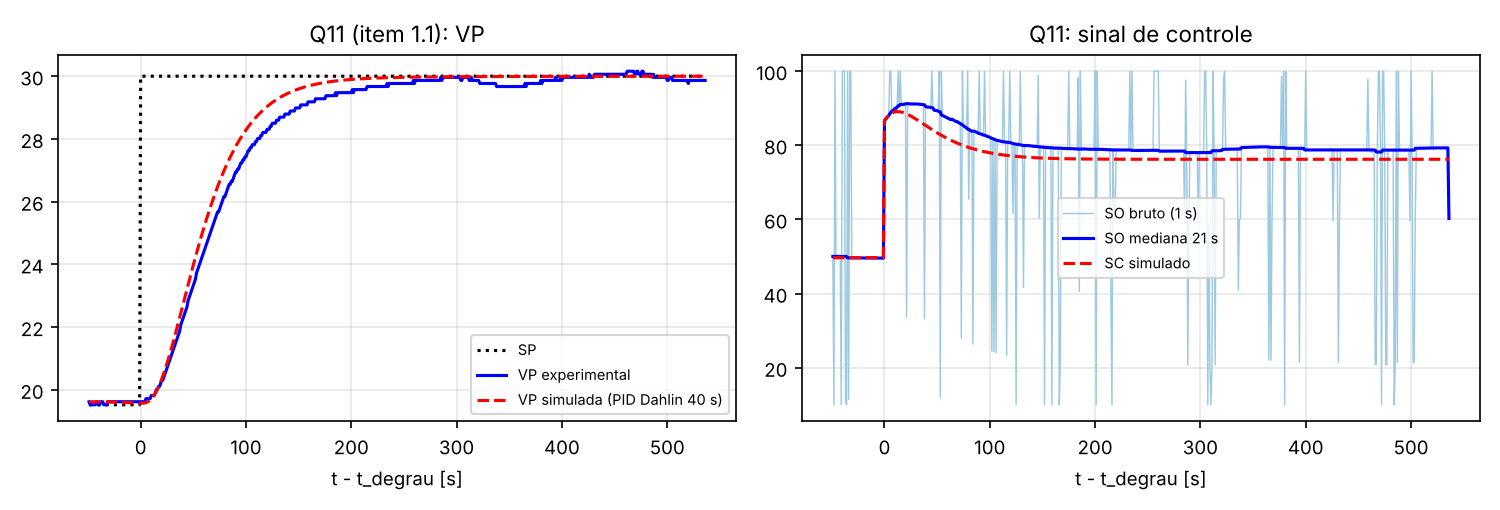
\includegraphics[width=.98\textwidth]{figs_exp/q11.png}\caption{Q11 (item 1.1). Esquerda: VP experimental (azul), SP e VP simulada. Direita: SO bruto (1 amostra/s, azul claro), mediana móvel de 21 s e SC simulado.}\end{figure}
\begin{center}\small
\begin{tabular}{lcc}\toprule & Experimento & Simulação (FT completa)\\\midrule
Instante em que a VP sobe 0,5 pt & 17 s & 16 s\\
$t_{28,3}$ / $t_{50}$ / $t_{63,2}$ & 43 / 64 / 79 s & 39 / 57 / 70 s\\
$t_{90}$ / $t_{95}$ / $t_{98}$ & 147 / 202 / 260 s & 118 / 142 / 174 s\\
Sobressinal (VP bruta) & 1,5\,\% ($VP_{max}=30{,}16$) & 0,0\,\%\\
SC médio em regime (últimos 300 s) & 75,4\,\% & 76,2\,\%\\
Erro VP: RMS / máximo & \multicolumn{2}{c}{0,38\,\% / 0,91\,\%}\\
Erro SC (mediana 21 s): RMS & \multicolumn{2}{c}{3,1\,\%}\\\bottomrule\end{tabular}\end{center}
\textbf{Interpretação.}
\begin{itemize}
\item \textbf{O sucesso da sintonia:} a VP chega ao SP sem sobressinal relevante ($\le1{,}5\,\%$ do degrau, no nível do ruído), com erro nulo em regime ($VP$ final $=29{,}9\text{--}30{,}0\,\%$), no formato previsto (sem oscilação, subida suave de 1ª ordem com atraso). O \emph{atraso aparente} de $\approx17$ s e o formato inicial são iguais aos simulados.
\item \textbf{A resposta experimental é um pouco mais lenta:} $t_{63,2}=79$ s contra 70 s (+13\,\%) e a cauda é mais lenta ($t_{98}=260$ s contra 174 s). As causas prováveis, em ordem: (i) as constantes de tempo reais do circuito são $\approx4$--6\,\% maiores que as calculadas (já constatado na identificação da 1ª parte, Seção 5.3); (ii) a rápida alternância do SO entre os limites (Seção~\ref{expruido}) \emph{retifica} o sinal: o SC médio aplicado ($75{,}4$) fica abaixo da mediana ($78{,}7$), o que atrasa o fechamento do último pedaço do degrau; (iii) tolerâncias dos $R$ e $C$.
\item \textbf{O SC concorda no valor médio e no formato:} salto inicial de $\approx37$ pontos, pico da mediana em $\approx91\,\%$ (simulado $88\,\%$) e queda até $\approx78$--79\,\% (simulado $76$). A diferença de $\sim3$ pontos entre mediana e simulação aparece porque o SO bruto é muito ruidoso; o que importa para a planta é a \emph{média}, e a média experimental ($75{,}4$) fica a $0{,}8$ ponto da simulada ($76{,}2$).
\end{itemize}
\begin{res}Item 1.1 verificado: a sintonia de Dahlin ($\tau_c=40$ s) leva a VP de $19{,}5$ a $30\,\%$ sem sobressinal significativo e sem erro em regime; VP experimental e simulada diferem por RMS de 0,38\,\% (3,6\,\% do degrau). O SC experimental tem o salto de $K_p\Delta SP$ previsto, mas é ruidoso (próxima seção).\end{res}

%------------------------------------------------------------------
\section{Por que o SO oscila entre $\approx$10\,\% e $\approx$99,9\,\% depois de fechar a malha? É preciso trocar para PI?}\label{expruido}
Esta é a observação mais importante dos ensaios: com a malha fechada, o gráfico do \texttt{SO} fica ``serrilhado'', com valores que pulam entre o limite inferior ($\approx10\,\%$) e o superior ($\approx99{,}9\,\%$), embora a VP seja suave. Vou mostrar, com os dados, \textbf{que isso não é instabilidade da malha}, qual é a causa, e o que fazer.

\subsection{Primeiro: não é instabilidade do laço}
\begin{itemize}
\item A \textbf{VP é suave}: em regime, o desvio-padrão da VP é de 0,13 ponto (Q11, $t>1900$ s), da ordem de 1 LSB do ADC ($0{,}0976\,\%$). Uma malha instável teria VP oscilando com amplitude crescente (como no ganho final do Z--N).
\item A \textbf{mediana} do SO é estável: desvio-padrão da mediana móvel $=1{,}2$ pontos (Q11), contra 17,5 do SO bruto.
\item O \textbf{valor médio} do SO está de acordo com a teoria: $(SP-\text{offset})/K=(30+0{,}26)/0{,}3971=76{,}2\,\%$ contra 75,4 medido.
\item Em Q11, 89,6\,\% das amostras do SO em malha fechada estão \emph{entre} os limites, só $2{,}4\,\%$ em 10\,\% e $8{,}0\,\%$ em 99,9\,\%: o SO fica no valor correto quase o tempo todo e dá \emph{picos isolados} ($\approx20\,\%$ das amostras).
\item Os picos já estão presentes com a \emph{malha recém-fechada e $SP=VP$} (Q11, t=1606--1650), quando o erro é praticamente zero e não há nada para ``instabilizar'' (veja a sequência do SO: \texttt{50, 50, 50, 10, 99,9, 50, 50, \ldots}).
\end{itemize}
\textbf{Conclusão parcial:} é um problema de \emph{ruído no sinal de controle}, e não de estabilidade.

\subsection{Segundo: a causa é a derivada atuando sobre a VP quantizada}
O ADC de 10 bits tem resolução de $100/1024=0{,}0976\,\%$ por degrau (LSB). A VP física varia lentamente (menos de $0{,}1\,\%$ por segundo em regime), então o valor lido é uma \textbf{escada}: fica constante por vários segundos e muda de 1 LSB de uma vez. Matematicamente, a derivada de uma escada é uma \emph{sequência de impulsos}. O termo derivativo é
\[
D(s)=\frac{K_d\,s}{\mu T_d\,s+1}\ \ \Rightarrow\ \ \text{resposta a um degrau de }\Delta V:\ \ u_D(t)=-\frac{K_d\,\Delta V}{\mu T_d}\,e^{-t/(\mu T_d)} .
\]
O sinal é negativo porque, no PI\_D, a derivada atua com sinal oposto sobre a VP. O \textbf{pico previsto por 1 LSB}, com o filtro funcionando como projetado ($\mu T_d=0{,}1\cdot11{,}11=1{,}11$ s), seria
\[
\frac{K_d\Delta V}{\mu T_d}=\frac{39{,}15\cdot0{,}0976}{1{,}11}=3{,}4\ \text{pontos},
\]
decaindo com constante de 1,11 s: um pequeno ``tremor'' de $\pm3$ pontos no SO. O ganho em alta frequência é $K_p(1+1/\mu)=38{,}8$: cada LSB vale $38{,}8\cdot0{,}0976=3{,}8$ pontos no máximo.

\textbf{O que os dados mostram é muito maior.} Nos registros com malha fechada:
\begin{center}\small
\resizebox{\textwidth}{!}{\begin{tabular}{lcccc}\toprule Registro & picos (|SO $-$ mediana|$>8$) & VP mudou 1 LSB & $P(\text{pico}\mid\text{LSB})$ & $P(\text{pico}\mid\text{sem LSB})$\\\midrule
Q11 ($t=1900$--2191) & 20\,\% das amostras & 14\,\% & 0,52 & 0,06\\
Q13a ($t=100$--560) & 46\,\% & 29\,\% & 0,64 & 0,27\\
Q12 ($t=620$--1075) & 42\,\% & 36\,\% & 0,56 & 0,22\\\bottomrule\end{tabular}}\end{center}
Na Q11 a probabilidade de haver um pico quando a VP muda de 1 LSB (na janela de $\pm1$ s) é $0{,}52$, \textbf{contra $0{,}06$ quando a VP não muda: um fator de 8,7}. Além disso, o \emph{sinal} é o da derivada sobre a VP: quando a VP sobe 1 LSB, o SO cai em média $26{,}1$ pontos; quando desce 1 LSB, o SO sobe em média $12{,}7$ (Figura~\ref{figruido}).
\begin{figure}[H]\centering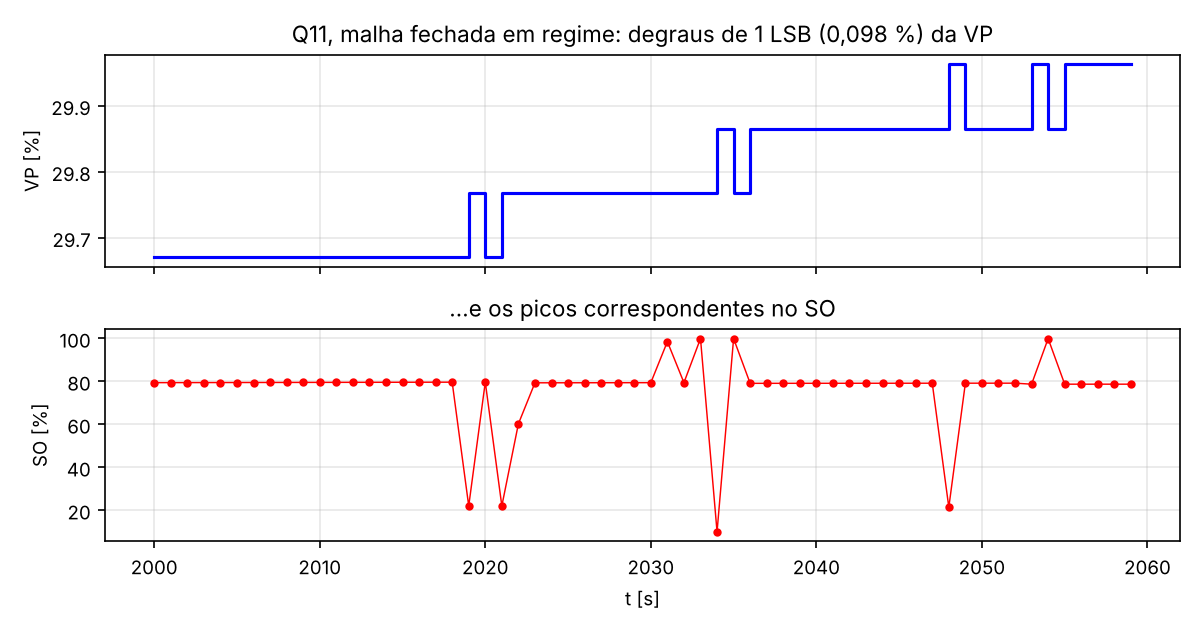
\includegraphics[width=.8\textwidth]{figs_exp/q11_ruido.png}\caption{Q11 em regime, malha fechada. Acima: a VP como escada de 1 LSB. Abaixo: o SO, com um pico a cada transição da VP.}\label{figruido}\end{figure}
\textbf{O tamanho do pico está inconsistente com o filtro de $\mu T_d=1{,}11$ s.} O pico típico medido (amostras não saturadas) tem mediana de 21 pontos, e muitos chegam a saturar (de $\sim79$ para 10 ou 99,9, isto é, $\gtrsim60$ pontos), contra os 3,4 pontos previstos. Como o ScadaBR só amostra o SO a cada 1 s (e um pico decai em fração de segundo), o pico real é ainda maior que o observado. Inverso: se o pico de 1 LSB é $K_d\Delta V/T_{ef}\gtrsim26$ pontos, então $T_{ef}\lesssim39{,}15\cdot0{,}0976/26=0{,}15$ s, muito menor que 1,11 s. Para comparação, uma derivada por \emph{diferença finita sem filtro}, com ciclo de execução (\emph{scan}) de 0,1 s, daria $K_d\Delta V/T_s=39{,}15\cdot0{,}0976/0{,}1=38$ pontos --- da ordem do observado.
\begin{alerta}Isto é uma \textbf{inferência}: não tenho o código do bloco PI\_D. O que os dados garantem é que (i) os picos acompanham as transições de 1 LSB da VP, com o sinal da derivada na VP, e (ii) são $\sim$10 vezes maiores do que o filtro $\mu=0{,}1$ permitiria. Isso indica que, no bloco usado, o filtro derivativo não está atuando como projetado (por exemplo, derivada calculada pela diferença entre amostras consecutivas do scan, com $\mu T_d$ muito curto na prática, ou $K_d$ digitado em unidade diferente da esperada). \textbf{Confirme:} (a) os valores de $K_d$, $T_d$ e $\mu$ digitados; (b) o tempo de ciclo do PLC; (c) o código do bloco.\end{alerta}

\subsection{Terceiro: por que o SO fica \emph{entre 10 e 99,9} e não entre $-\infty$ e $+\infty$}
Os picos de dezenas de pontos são cortados pelos limites do SC, $\approx10\,\%$ e $\approx99{,}94\,\%$ (Seção~\ref{expdados}). Por isso o gráfico parece ``instável entre 0 e 99'': na verdade é entre \textbf{10 e 99,94}, os limites de saturação. O limite inferior em 10\,\% (e não 0\,\%) aparece no mínimo $9{,}99485$ de todos os arquivos.

\subsection{Por que a planta ``não liga'' para os picos --- e por que ainda assim eles importam}
O circuito RC é um filtro passa-baixa de 3ª ordem (polos em $1/68{,}7$; $1/16$; $1/10{,}4$ s$^{-1}$): um pico de 60 pontos que dura $\sim0{,}2$ s muda a VP em centésimos de ponto. Por isso a VP fica suave. Mesmo assim, os picos \textbf{importam}:
\begin{enumerate}
\item \textbf{Desgaste/inadequação do atuador:} o SO muda entre os limites em até 14\,\% das amostras (Q12: $13{,}9\,\%$ das amostras em 10\,\%).
\item \textbf{Retificação pela saturação:} um pico para cima quando o SC médio está no limite inferior (10\,\%), ou para baixo no limite superior, \emph{desloca a média} aplicada. Exemplo (Q13b): no patamar em que o SC deveria estar fixo em 99,94\,\% o SO médio foi $96{,}6\,\%$; como $K\approx0{,}396$, isso reduz a VP máxima em $0{,}396\cdot3{,}3=1{,}3$ ponto ($VP_{max}=38{,}16$ medido, contra $39{,}39$ do patamar sem ruído, Q13a). Em outro exemplo, depois da queda do SP (Q13b, $t=550$--600 s), o SC deveria ficar em 10\,\% mas o SO médio ficou em $\approx25$--35\,\%, o que fez a VP cair mais devagar que na simulação.
\item \textbf{Comparação SC experimental $\times$ simulado:} o SO bruto não é comparável com o SC simulado (que é a média). Por isso uso a mediana móvel nas figuras e quantifico a diferença.
\end{enumerate}

\subsection{É necessário trocar para um PI?}
\textbf{Resposta direta: não é necessário para a \emph{estabilidade} (a malha já está estável), mas é a solução mais segura para eliminar o ruído do SC, e a simulação mostra que, para esta planta, a resposta quase não muda.}

\textbf{Por quê?} A derivada compensa fase perto da frequência de cruzamento; aqui o atraso é pequeno em relação à constante de tempo ($t_0/\tau=25{,}9/78{,}0=0{,}33$) e a malha tem folga de fase de sobra. Na Tabela 7-4.1, o PI vem da \emph{mesma} dedução do PID (Dahlin com Padé de ordem zero, $e^{-t_0s}\approx1-t_0s$):
\[
C(s)=\frac{\tau s+1}{K\,s\,(\tau_c+t_0)}\ \Rightarrow\ K_c=\frac{\tau}{K(\tau_c+t_0)}=\frac{78{,}03}{0{,}3918\,(40+25{,}92)}=3{,}02\ \%\mathrm{SC}/\%\mathrm{VP},\qquad \tau_I=\tau=78{,}03\ \mathrm{s}.
\]
(Compare com o PID: $K_p=3{,}523$ e $T_i=90{,}99$ s.) Simulei os candidatos na FT completa (degrau $20\to30\,\%$; $\Delta t=0{,}05$ s):
\begin{center}\small
\resizebox{\textwidth}{!}{\begin{tabular}{lccccccc}\toprule Controlador & $PM$ & $GM$ & sobress. & $t_{63}$ & $t_s$ & pico SC & ganho HF $\to$ pontos de SC/LSB\\\midrule
PID Dahlin, $\mu=0{,}1$ (usado) & $81{,}4^\circ$ & 59,7 & 0\,\% & 70 s & 172 s & 87,9\,\% & 38,8 $\to$ 3,8\\
PID mesma sintonia, $\mu=0{,}5$ & $81{,}5^\circ$ & 16,0 & 0\,\% & 70 s & 178 s & 88,5\,\% & 10,6 $\to$ 1,0\\
PID mesma sintonia, $\mu=1{,}0$ & $81{,}5^\circ$ & 10,9 & 0,1\,\% & 69 s & 185 s & 89,0\,\% & 7,0 $\to$ 0,7\\
\textbf{PI Dahlin} ($K_c=3{,}02$; $T_i=78{,}03$) & $70{,}1^\circ$ & 9,5 & 0\,\% & 71 s & 145 s & 86,7\,\% & \textbf{3,0 $\to$ 0,3}\\\bottomrule\end{tabular}}\end{center}
\begin{figure}[H]\centering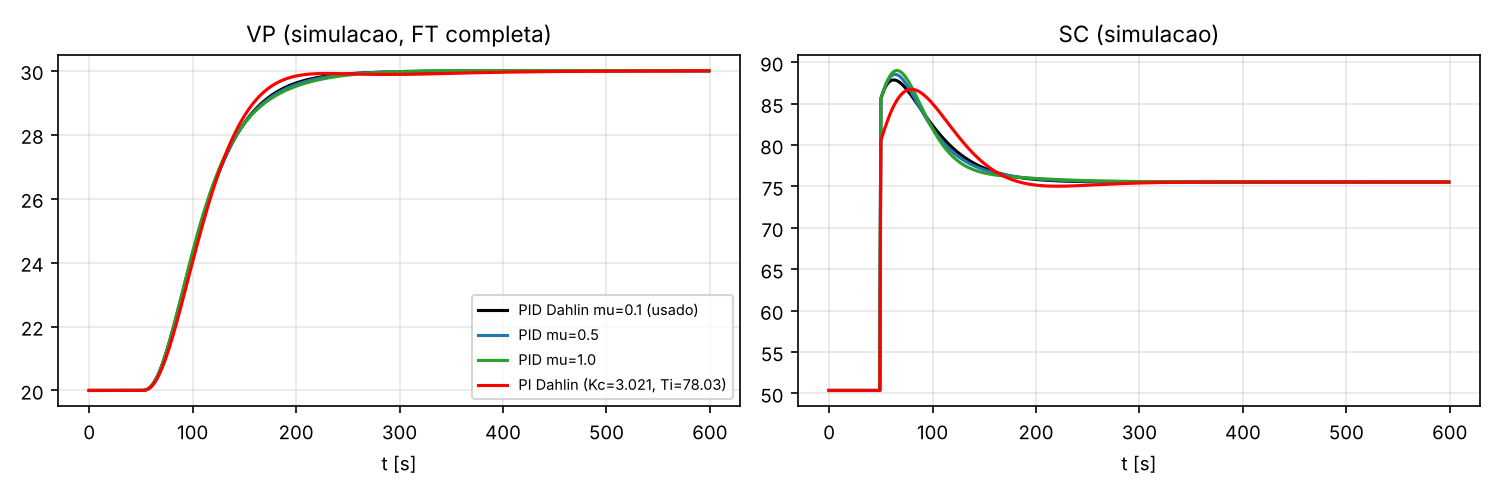
\includegraphics[width=.98\textwidth]{figs_exp/pi_x_pid.png}\caption{Simulação (FT completa): PID Dahlin ($\mu=0{,}1$, usado), PID com $\mu=0{,}5$ e $1{,}0$, e PI Dahlin. As quatro respostas praticamente coincidem.}\end{figure}
\begin{res}O PI de Dahlin dá praticamente a mesma VP ($t_{63}=71$ s contra 70 s; acomoda até mais rápido, 145 s contra 172 s), com $PM=70^\circ$ e $GM=9{,}5$ (folga confortável), e reduz o ganho de alta frequência de 38,8 para 3,0, isto é, \textbf{o efeito de 1 LSB no SC cai de 3,8 para 0,3 ponto (pelo menos 10 vezes menos), sem filtro nenhum}.\end{res}
\textbf{Recomendação (para relatório e prova):}
\begin{enumerate}
\item \textbf{Manter o relatório do item 1.1 como PID} (é o que o enunciado pede: ``sintonia de PID segundo a Tabela 7-4.1'') e \emph{documentar} o ruído com esta análise (causa, evidência e solução).
\item \textbf{Alternativa validada: PI de Dahlin} ($K_p=3{,}02$; $T_i=78{,}03$ s; $K_d=0$). É a resposta à pergunta ``precisa mudar para PI?'': não é obrigatório, mas \emph{funciona} e remove o ruído. Se for repetir o ensaio, \textbf{rode também um registro com PI} e confronte VP e SC (o SC do PI deve ficar limpo: desvio-padrão do SO próximo de 1 ponto, como a mediana atual).
\item \textbf{Se quiser manter a derivada}: (a) aumente $\mu$ (0,5 a 1,0) \emph{somente se} o bloco realmente usar o filtro (verifique o código); (b) filtre a VP antes do PID (média de 8 leituras do ADC ou um passa-baixa digital com constante $\approx1$ s); (c) aumente o tempo de execução do bloco PID (por exemplo 0,5 s: o pico por LSB cai para $39{,}15\cdot0{,}0976/0{,}5=7{,}6$ pontos); (d) filtro RC analógico na entrada do ADC.
\end{enumerate}
\begin{just}\textbf{Como confirmar o diagnóstico rapidamente na bancada:} repita o item 1.1 com $K_d=0$ (PI). Se a causa é a derivada, o SO deixa de ter picos (SO bruto $\approx$ mediana). Se ainda tiver picos, a causa está em outro ponto (por exemplo, o termo P e o ruído muito alto do ADC); nesse caso meça o ruído do ADC com a saída fixa.\end{just}

%------------------------------------------------------------------
\section{Item 1.2 experimental (Q12): transferência manual$\to$automático sem VP-tracking}
\subsection{Objetivo (seção 5-3.3 do livro)}
O \emph{bumpless VP-tracking} faz o SP acompanhar a VP enquanto o controlador está em manual. Assim, quando se passa para automático, $e=SP-VP=0$ e o SC não sofre salto. Sem o tracking, se o SP estiver diferente da VP no instante da transferência, o termo proporcional produz um salto $\Delta SC=K_p\,(SP-VP)$ (``bump'') e a VP é puxada bruscamente.
\subsection{O que foi feito}
\begin{enumerate}
\item Manual: $SO=10{,}37\to20{,}0\,\%$ e a VP sobe até $7{,}71\,\%$. Nesse período o \textbf{SP ficou em 0\,\%} (não acompanhou a VP: tracking desligado; compare com a Q11, em que o SP seguia a VP).
\item Em $t=577$ s o operador ajusta $SP=16{,}0\,\%$ (com a VP em $7{,}71$, isto é, $SP-VP=8{,}29$).
\item Em $t=593$ s passa para automático (SO manual $=20{,}0\,\%$).
\end{enumerate}
\subsection{Resultado}
\textbf{Previsto:} $\Delta SC=K_p(SP-VP)=3{,}523\cdot(16{,}00-7{,}71)=29{,}2$ pontos, isto é, $SC\approx20{,}0+29{,}2=49{,}2\,\%$ logo após a transferência.\\
\textbf{Medido:} $SO(593\text{--}600)=\{20{,}0;\ 30{,}1;\ 10{,}0;\ 49{,}7;\ 49{,}9;\ 99{,}9;\ 50{,}4;\ 31{,}5\}$ e \textbf{mediana de 595 a 615 s $=50{,}2\,\%$}: o SO saltou de $20$ para $\approx50\,\%$ (+$30$ pontos), exatamente o salto previsto (a diferença de 1 ponto é o termo integral e o ruído). Os valores 10, 30 e 99,9 são os picos da derivada da Seção~\ref{expruido}.
\begin{figure}[H]\centering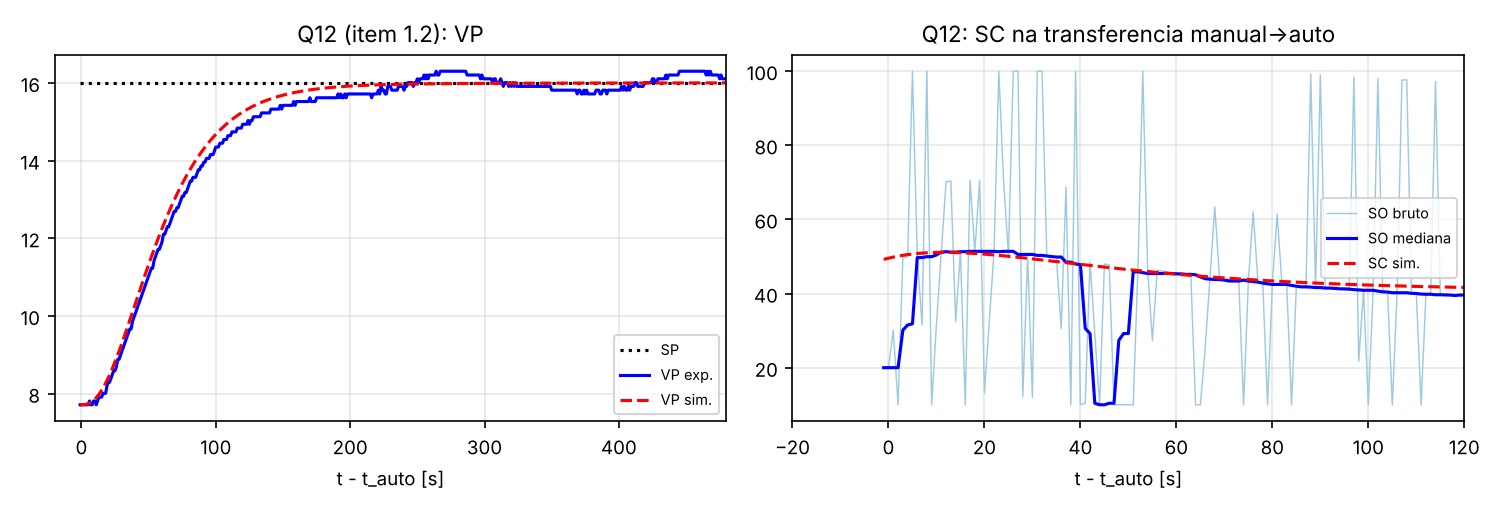
\includegraphics[width=.98\textwidth]{figs_exp/q12.png}\caption{Q12 (item 1.2). Esquerda: VP experimental e simulada após a transferência. Direita: SO na transferência (salto de $\sim30$ pontos em $t=0$) e SC simulado.}\end{figure}
A VP, que estava parada em $7{,}71\,\%$, sobe imediatamente em direção a 16\,\% como se o operador tivesse dado um degrau grande de SP, sem que o SC tenha sido ``pedido'': é o \emph{problema} que o tracking evita. A simulação (com a mesma sintonia, $SP=16$, $VP_0=7{,}71$, $SC_0=20$) reproduz a VP com RMS de $0{,}24\,\%$ e erro máximo de $0{,}45\,\%$ (VP máxima: 16,30 medida, 16,00 simulada).
\subsection{Comparação com o caso com VP-tracking (Q11)}
Na Q11, a transferência foi feita com $SP=VP=19{,}52$: o SO ficou em $\approx50\,\%$ (mediana $49{,}6\,\%$), sem salto (as oscilações isoladas são os picos de ruído). Resumo:
\begin{center}\small\begin{tabular}{lcc}\toprule & Sem tracking (Q12) & Com tracking (Q11)\\\midrule
$SP-VP$ na transferência & $+8{,}29$ & $0{,}00$\\ Salto previsto $K_p(SP-VP)$ & $+29{,}2$ & $0$\\ Salto medido (mediana do SO) & $+30$ (20$\to$50,2) & $\approx0$ (50,0$\to$49,6)\\\bottomrule\end{tabular}\end{center}
\begin{res}O experimento reproduz o problema: sem VP-tracking, a transferência manual$\to$automático com $SP\neq VP$ produz um salto de SC igual a $K_p(SP-VP)$ ($+30$ pontos medido, $+29{,}2$ previsto). Com tracking (Q11), não há salto.\end{res}

%------------------------------------------------------------------
\section{Item 1.3 experimental (Q13a e Q13b): anti reset windup}
\subsection{Fundamentos}
\textbf{O que é o windup.} A ação integral soma o erro no tempo, $I=K_i\!\int e\,dt$. Quando o atuador satura (SC no limite), o erro não consegue ser zerado, e a integral \emph{continua crescendo}, ``carregando'' um valor muito maior do que o atuador pode usar. Quando o SP volta a um valor alcançável, o erro muda de sinal, mas a integral só decresce à taxa $K_i|e|$ --- demora até que $u=K_pe+I$ saia da saturação. Durante esse tempo, a VP fica fora do controle.

\textbf{Anti reset windup} (seção 5-3.4): interromper a integração (ou descontar o excesso) enquanto o SC está saturado, de modo que $I$ fique perto do valor necessário no momento em que o SP deixa de ser inalcançável. A implementação por \emph{clamping} usada na simulação: $I[k+1]=I[k]+K_ie\Delta t$ \emph{exceto} se $u>u_{max}$ e $e>0$ ou $u<u_{min}$ e $e<0$.

\subsection{Alcance máximo e como o experimento foi planejado}
Com SC máximo de $99{,}94\,\%$: $VP_{max}=0{,}3963\cdot99{,}94-0{,}262=39{,}4\,\%$ (medido: $39{,}33$--$39{,}39\,\%$ em Q13a). Logo, $SP=55\,\%$ é \emph{inalcançável} por uma larga margem e o SC fica saturado em 99,94\,\% durante todo o tempo em que o SP está em 55\,\%.

\subsection{Linha do tempo extraída dos dados}
\begin{center}\small
\begin{tabular}{lcc}\toprule Evento & Q13a (sem AW) & Q13b (com AW)\\\midrule
Malha fechada (SO manual 20\,\%) & $t=820$ s ($VP=7{,}5$) & $t=38$ s ($VP=6{,}05$)\\
SP $\to55\,\%$ & $t=822$ s & $t=43$ s\\
Tempo com SP inalcançável & 449 s & 501 s\\
VP máxima no patamar & 39,33\,\% & 38,16\,\%\\
SP $\to20\,\%$ & $t=1271$ s & $t=544$ s\\\bottomrule\end{tabular}\end{center}
\begin{figure}[H]\centering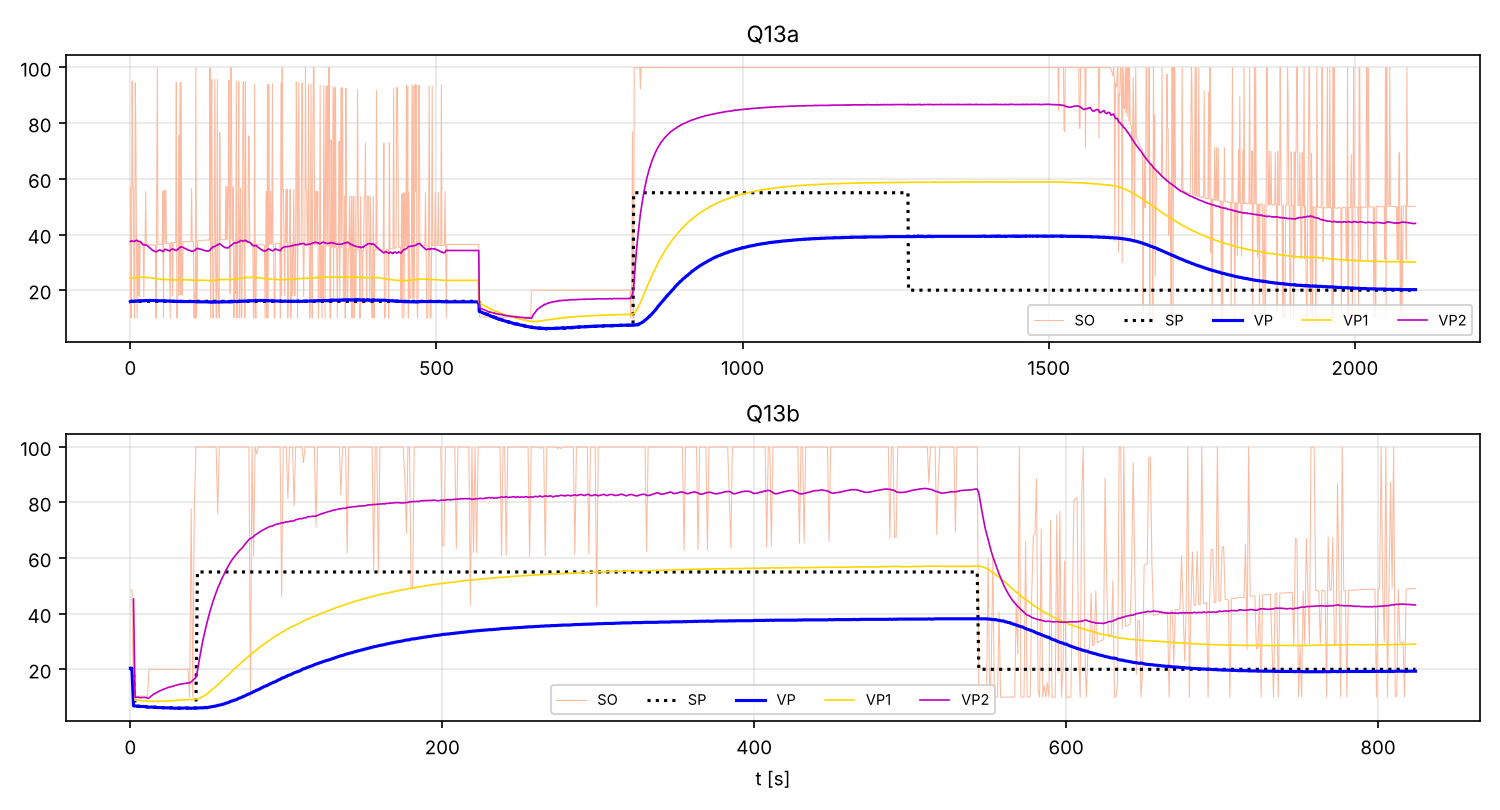
\includegraphics[width=.98\textwidth]{figs_exp/q13_completo.png}\caption{Registros completos de Q13a (acima) e Q13b (abaixo): SO, SP, VP, VP1 e VP2.}\end{figure}
\subsection{Resultado: o que acontece depois que o SP volta a 20\,\%}
\begin{figure}[H]\centering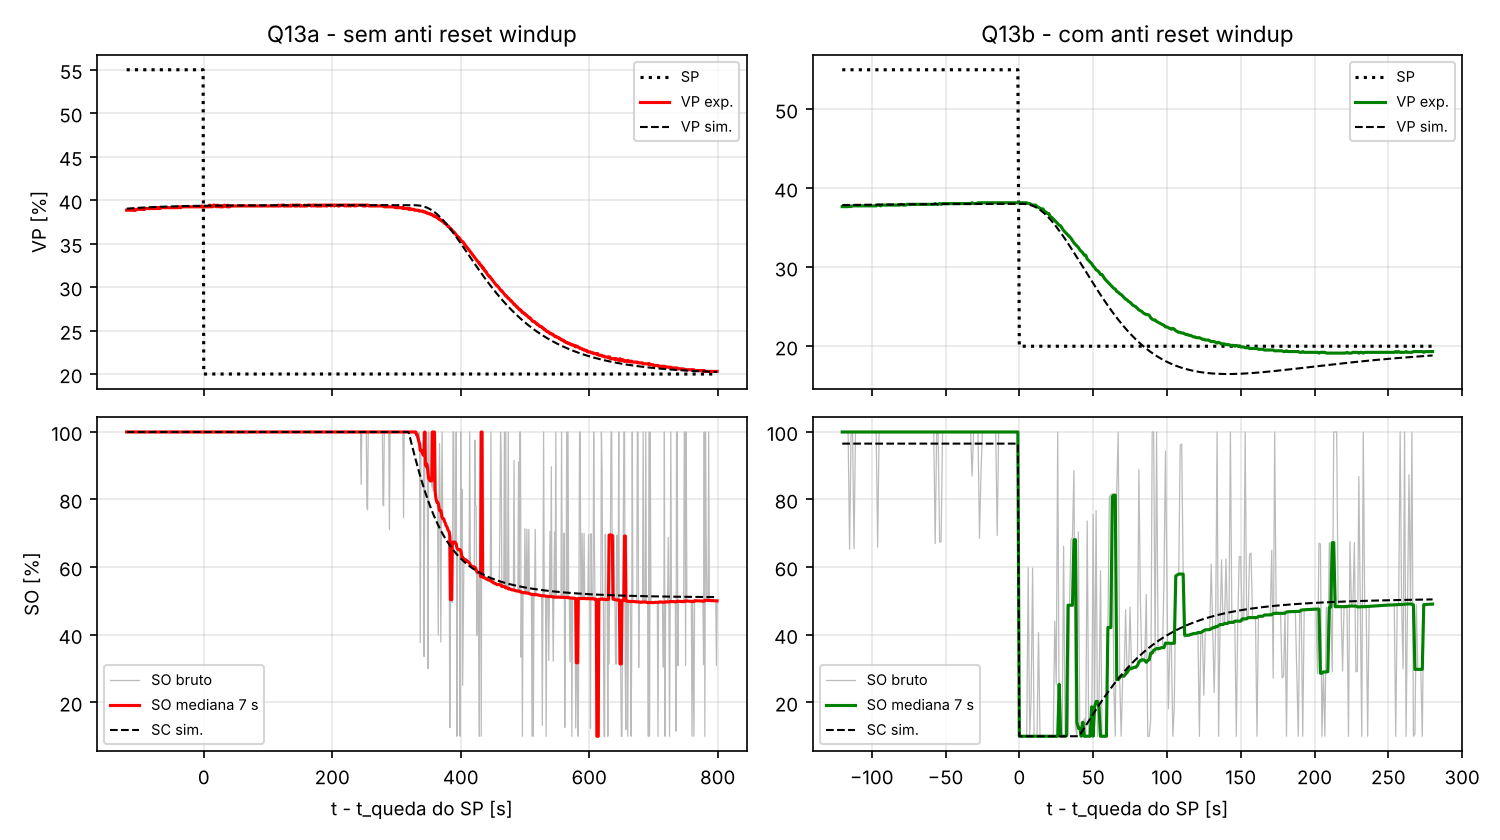
\includegraphics[width=.98\textwidth]{figs_exp/q13.png}\caption{Q13 alinhado no instante da queda do SP (t=0). Esquerda: sem anti-windup. Direita: com anti-windup. Linhas tracejadas: simulação.}\end{figure}
\begin{center}\small
\resizebox{\textwidth}{!}{\begin{tabular}{lcc}\toprule Medida (a partir da queda do SP) & Q13a: sem AW & Q13b: com AW\\\midrule
O SO sai da saturação (mediana $<95\,\%$) & \textbf{337 s} depois & \textbf{0 s} (imediato)\\
A VP começa a cair (0,5 ponto abaixo do máximo) & \textbf{342 s} depois & \textbf{13 s} depois\\
A VP fica dentro de $\pm1$ ponto de 20\,\% & 700 s & 123 s\\\midrule
Simulação: SC sai da saturação & 326 s (sem AW) & 0 s (com AW)\\
Simulação: VP cai 0,5 ponto & 355 s (sem AW) & 12 s (com AW)\\
Erro RMS VP experimental $\times$ simulado & \textbf{0,43\,\%} (sem AW) / 11,0\,\% (com AW) & \textbf{1,62\,\%} (com AW) / 9,2\,\% (sem AW)\\\bottomrule\end{tabular}}\end{center}
\textbf{Interpretação.}
\begin{itemize}
\item \textbf{Sem anti-windup (Q13a):} depois da queda do SP, o SO permanece em 99,94\,\% por \textbf{337 s} e a VP permanece em 39,3\,\% por $\approx340$ s, \emph{mesmo com o SP em 20\,\% e erro de $-19$ pontos}. O controlador está ``cego'': o integrador acumulou, durante os 449 s de saturação, um valor muito acima do que o atuador entrega. Só depois que o integrador desce é que $u=K_pe+I$ cai abaixo de 99,94 e a VP finalmente começa a descer. Só chega a $\pm1$ ponto de 20\,\% depois de $\approx700$ s.
\item \textbf{Com anti-windup (Q13b):} o SO deixa a saturação \emph{imediatamente} e a VP começa a cair 13 s depois (o atraso de 13 s é a dinâmica do circuito: $\Vc3$ é de 3ª ordem e só começa a cair depois que $\Vc1$ e $\Vc2$ caem), chegando a $\pm1$ ponto de 20\,\% em 123 s, \textbf{5,7 vezes mais rápido} que sem anti-windup (700 s).
\item \textbf{Quantificando o windup (conta feita com os dados):} durante os 449 s com SP$=55$ (erro positivo de 47 pontos no início e 16 no fim), a integral acumulou $I=20+K_i\sum e\,\Delta t=20+0{,}03872\cdot\sum(SP-VP)=414$ pontos de SC (em regime final, para $SP=20$, bastariam $I\approx(20+0{,}26)/0{,}3971=51$). Logo após a queda do SP, o erro vale $20-39{,}3=-19{,}3$ e o termo proporcional $K_pe=3{,}523\cdot(-19{,}3)=-68$; o controlador só sai da saturação quando $u=K_pe+I<99{,}94$, isto é, $I<168$. A integral precisa descer $414-168=246$ pontos à taxa $K_i|e|=0{,}03872\cdot19{,}3=0{,}75$ ponto/s:
\[t_{saida}\approx\frac{246}{0{,}75}=328\ \mathrm{s}\qquad(\text{medido: }337\ \mathrm{s}).\]
A estimativa independente da simulação (328 s) confere com o dado (337 s): o atraso é exatamente o tempo de ``desenrolar'' o integrador.
\item \textbf{A simulação reproduz cada caso com a estrutura certa:} o modelo \emph{sem} anti-windup reproduz a Q13a (RMS 0,43\,\%; SO sai da saturação em 326 s contra 337 s medidos); o modelo \emph{com} anti-windup (clamping) reproduz a Q13b (RMS 1,62\,\%, mesmo tempo de saída da saturação, VP caindo em 12 s contra 13 s). Trocando as estruturas, o erro explode (11,0\,\% e 9,2\,\%): a simulação \emph{discrimina} qual é qual, o que confirma que a Q13a é sem proteção e a Q13b com proteção.
\item \textbf{Diferenças residuais na Q13b} (RMS 1,6\,\%, concentrado depois da queda do SP): (i) o SC médio no patamar saturado foi 96,6\,\% e não 99,94\,\% (retificação do ruído da derivada); (ii) depois da queda, o SC deveria ficar em 10\,\%, mas o SO médio foi 25--35\,\% pelos picos, o que retarda a queda da VP (a VP experimental cai mais devagar que a simulada, sem o \emph{undershoot} de $\approx3$ pontos que a simulação com clamping prevê). Ambos os efeitos são consequência do mesmo ruído da Seção~\ref{expruido}.
\end{itemize}
\begin{res}O experimento reproduz o problema do windup: sem anti-windup, depois de 449 s com o SP inalcançável, a VP fica \textbf{340 s} presa no valor máximo ($39{,}3\,\%$) e só atinge $20\pm1\,\%$ em $\approx700$ s; com anti-windup o SC sai da saturação na hora, a VP reage em 13 s (dinâmica da planta) e chega a $20\pm1\,\%$ em 123 s.\end{res}

%------------------------------------------------------------------
\section{Conclusões dos experimentos da Questão 1}
\begin{enumerate}
\item \textbf{Modelo validado no dia do ensaio:} inclinação estática $0{,}3963$ (teórico $0{,}3971$), offset de $-0{,}26$ ponto e dinâmica reproduzida com RMS de 0,2--0,8\,\% quando a planta é excitada com o SO medido.
\item \textbf{Item 1.1:} a sintonia de Dahlin ($\tau_c=40$ s) funcionou: sem sobressinal significativo, erro nulo em regime, salto de SC igual a $K_p\Delta SP$. A resposta experimental é $\approx13\,\%$ mais lenta que a simulada ($t_{63}$ de 79 contra 70 s), coerente com a diferença de 4--6\,\% nas constantes de tempo já observada e com o ruído do SC.
\item \textbf{SO ``instável'':} é \textbf{ruído no sinal de controle}, não instabilidade da malha: a derivada amplifica os degraus de 1 LSB (0,098\,\%) do ADC (probabilidade de pico 8,7 vezes maior nas transições da VP); os picos, de dezenas de pontos, são cortados pelos limites $\approx10$ e $\approx99{,}94\,\%$ do SC. O filtro $\mu=0{,}1$ deveria limitar o pico a $\approx3{,}4$ pontos, mas os picos observados são $\sim10$ vezes maiores: o filtro não atua como projetado no bloco usado.
\item \textbf{PI:} não é obrigatório para a estabilidade, mas é a correção mais simples: o PI de Dahlin ($K_c=3{,}02$; $T_i=78{,}03$ s) dá VP praticamente idêntica ($t_{63}=71$ s, $PM=70^\circ$) com o ganho de alta frequência 13 vezes menor. Recomendo registrar um ensaio com PI para confirmar.
\item \textbf{Item 1.2:} sem VP-tracking, o SC saltou $+30$ pontos na transferência (previsto $K_p(SP-VP)=29{,}2$); com tracking (Q11), não há salto.
\item \textbf{Item 1.3:} sem anti-windup a VP fica presa em $39{,}3\,\%$ por $\approx340$ s depois da queda do SP, e só chega a $20\pm1\,\%$ em 700 s; com anti-windup, em 123 s. A simulação com a estrutura correta reproduz cada ensaio com RMS $\le1{,}6\,\%$.
\end{enumerate}
\textbf{Limitações:} (i) a sintonia usada (Dahlin) foi inferida do salto do SO, não de anotação; (ii) os picos de SO são amostrados a 1 s e portanto subestimados; (iii) o código do bloco PID não foi analisado, o que impede afirmar a causa exata do filtro derivativo ineficaz; (iv) só há um ensaio de cada tipo, sem repetição.

%==================== PARTE B: RUÍDO NO SO, PROGRAMA DO PLC E CORREÇÃO ====================
\section{O programa do PLC (\texttt{Prova2.st}): o que ele realmente faz}\label{secst}
O programa é um PI\_D paralelo construído com blocos da biblioteca IEC 61131-3 e executado por uma tarefa de \textbf{20 ms} (\texttt{TASK task0(INTERVAL := T\#20ms)}). A listagem completa está no Apêndice~\ref{apcodigos}. Resumo, bloco a bloco:
\begin{center}\small
\begin{longtable}{p{3.4cm}p{11.2cm}}
\toprule \textbf{Elemento} & \textbf{O que faz (e por quê importa)}\\\midrule\endhead
Escalas & \texttt{VP}, \texttt{SP} e \texttt{SO} são \texttt{UINT} (0--65535). Multiplicar por $0{,}001525$ dá \%. O ADC de 10 bits do Arduino entra como múltiplos de 64, logo \textbf{1 LSB $=64\cdot0{,}001525=0{,}0976\,\%$}.\\
\texttt{MF} (\texttt{\%QX0.0}) & Modo: \texttt{MF=1} = automático (malha fechada); \texttt{MF=0} = manual. Em manual o erro é forçado a 0.\\
Erro & $e=(SP-VP)\cdot M\_ACAO$ ($M\_ACAO=1$). Zona morta: se $|e|<0{,}09$, $e=0$. Como o menor erro não nulo é 1 LSB $=0{,}0976>0{,}09$, \textbf{a zona morta nunca atua}.\\
Proporcional & $K_p\,e$, com \texttt{kp = 3.523}.\\
Integral & Bloco \texttt{INTEGRAL}, \texttt{XIN = ki$\cdot e$} (zero se \texttt{STOP\_INTGR}), \texttt{CYCLE = 500 ms}, reinicia em 0 quando \texttt{MF=0}; a saída é multiplicada por $0{,}04$. Como o bloco é executado a cada 20 ms mas ``acredita'' em 500 ms, o ganho $0{,}04=0{,}02/0{,}5$ corrige a escala: o resultado é $\int K_i\,e\,dt$ com \texttt{ki = 0.03872}.\\
Derivada & \texttt{XIN} $=-k_d\cdot VP$ (zero em manual), bloco \texttt{DERIVATIVE} com \texttt{CYCLE = 500 ms}, saída multiplicada por $25$ ($=0{,}5/0{,}02$, mesma correção de escala), \texttt{kd = 39.16}. \textbf{Não existe filtro $\mu T_d$} no programa. O bloco \texttt{DERIVATIVE} da biblioteca padrão usa a diferença de 4 pontos
\[\tfrac{3\,(x_k-x_{k-3})+x_{k-1}-x_{k-2}}{10\,T_s},\ T_s=20\ \mathrm{ms}.\]\\
Bias (bumpless da saída) & \texttt{SO\_AUX := SO} em manual, mantendo o último valor em automático. O SC é $SO_{manual}+K_pe+I+D$. Logo, ao fechar a malha com $e=0$, o SC continua igual ao SO manual (transferência sem salto), e a integral parte de zero.\\
VP-tracking & \texttt{SP := SEL(MF, VP, SP)}: em manual o SP é sobrescrito pela VP. É o mecanismo do item 1.2.\\
Anti-windup & \texttt{STOP\_INTGR := (u $\ge100$) OR (u $\le10$)}; quando verdadeiro, \texttt{XIN} da integral vale 0: \textbf{a integral congela enquanto o SC está saturado} (não é o \emph{clamping} condicionado ao sinal do erro). É o mecanismo do item 1.3.\\
Saturação & \texttt{LIMIT(10.0, u, 100.0)}: SC entre 10 e 100\,\% (\texttt{SC = u$\cdot655{,}35$}).\\
2GL & \texttt{FF2GL} acumula $K_p(1-\mathtt{alfa})\,\Delta SP$ a cada mudança de SP em automático e é \emph{subtraído} de $u$. \texttt{alfa = 1} $\Rightarrow$ PI\_D comum (Seção~\ref{alfaplc}).\\\bottomrule
\end{longtable}\end{center}
\subsection{A derivada de 4 pontos sem filtro: resposta a 1 LSB}\label{deriv4}
Seja um degrau de $\Delta V=1$ LSB $=0{,}0976\,\%$ na VP lida, ocorrendo no scan $k_0$ (a entrada do bloco é $-k_dVP$). Aplicando a fórmula de 4 pontos, a saída vale
\[
D_{k_0}=-\frac{3\,k_d\Delta V}{10T_s},\quad D_{k_0+1}=-\frac{4\,k_d\Delta V}{10T_s},\quad D_{k_0+2}=-\frac{3\,k_d\Delta V}{10T_s},\quad D_{k_0+3}=0,
\]
isto é, um pulso de 3 scans (60 ms) com área $k_d\Delta V$. Com os números do programa,
\[
u_0\equiv\frac{k_d\,\Delta V}{10\,T_s}=\frac{39{,}16\cdot0{,}0976}{10\cdot0{,}02}=19{,}1\ \text{pontos},\qquad\text{pulsos: }57{,}3;\ 76{,}4;\ 57{,}3\ \text{pontos de SC}.
\]
(Se existisse o filtro $\mu=0{,}1$ do projeto, o pico seria $k_d\Delta V/(\mu T_d)=3{,}4$ pontos.) Qualquer combinação de degraus de $\pm1$ LSB em scans vizinhos produz saídas que são múltiplos inteiros de $u_0=19{,}1$ pontos (coeficientes $3,1,-1,-3$ vezes $u_0$).

\subsection{O 2GL do programa e a tradução do $\alpha$ do TCC}\label{alfaplc}
Em automático, a cada mudança de SP o programa soma a \texttt{FF2GL} $K_p(1-\mathtt{alfa})\Delta SP$ e subtrai o total de $u$. Com isso, a ação proporcional sobre o SP fica
\[
K_p\,\Delta SP-K_p(1-\mathtt{alfa})\Delta SP=\mathtt{alfa}\cdot K_p\,\Delta SP,
\]
isto é, \textbf{ponderação do SP no termo proporcional com peso $b=\mathtt{alfa}$}, com a integral sobre o erro completo. No TCC (e no CLP Omron), o filtro do SP é $C_f=\dfrac{(1-\alpha)T_is+1}{T_is+1}$ e
\[
C_f\cdot PI=K_p\frac{T_is+1}{T_is}\cdot\frac{(1-\alpha)T_is+1}{T_is+1}=K_p\Big[(1-\alpha)+\frac{1}{T_is}\Big],
\]
ou seja, o mesmo comportamento com peso $b=1-\alpha_{TCC}$. \textbf{Os dois são equivalentes com $\mathtt{alfa}_{PLC}=1-\alpha_{TCC}$.} Consequências:
\begin{itemize}
\item O $\alpha_{TCC}=0{,}64$ escolhido no item 2.1 corresponde a \textbf{\texttt{alfa = 0.36} no programa}.
\item $\mathtt{alfa}=1$ é o PI\_D comum (valor inicial do programa); $\mathtt{alfa}=0$ dá P e D sobre a VP e só a integral sobre o erro: é o \textbf{I\_PD} (item 4.2).
\end{itemize}
\subsection{Pontos de atenção do programa (encontrados na leitura)}
\begin{enumerate}
\item \textbf{Derivada sem filtro:} amplifica o ruído de quantização do ADC (Seção~\ref{expruido}).
\item \textbf{Derivada zerada em manual:} \texttt{Kd\_VP\_PERC := SEL(MF, 0.0, $-k_d\cdot VP$)}. Ao fechar a malha, a entrada do bloco ``salta'' de 0 para $-k_dVP\approx-760$, o que gera um pulso de 3 scans que leva o SC a 10\,\% (saturado) \emph{em todo fechamento de malha} (visto nos dados: Seções~\ref{expq11} e \ref{expq12}).
\item \textbf{Anti-windup por congelamento:} quando picos de derivada saturam $u$ em um scan, a integral congela naquele scan; com picos frequentes, a integral perde parte do tempo e a resposta fica mais lenta (Seção~\ref{expq11}).
\item \textbf{Zona morta de 0,09:} menor que 1 LSB, nunca atua.
\end{enumerate}

%------------------------------------------------------------------
\section{Por que o SO oscila entre $\approx$10\,\% e $\approx$99,9\,\% depois de fechar a malha? É preciso trocar para PI?}\label{expruido}
Esta é a observação mais importante dos ensaios: com a malha fechada, o gráfico do \texttt{SO} fica ``serrilhado'', com valores que pulam entre o limite inferior ($10\,\%$) e o superior ($\approx99{,}94\,\%$), embora a VP seja suave. Com o código do PLC em mãos é possível \textbf{explicar a causa com exatidão} e não só indicá-la.
\subsection{Primeiro: não é instabilidade do laço}
\begin{itemize}
\item A \textbf{VP é suave}: desvio-padrão de 0,13 ponto em regime (Q11, $t>1900$ s), da ordem de 1 LSB. Uma malha instável teria VP oscilando com amplitude crescente.
\item A \textbf{mediana} do SO é estável (desvio-padrão da mediana móvel: 1,2 ponto, contra 17,5 do SO bruto) e o \textbf{valor médio} do SO concorda com a teoria: $(SP-\text{offset})/K=(30+0{,}26)/0{,}3971=76{,}2\,\%$ contra 75,4 medido.
\item Na Q11, 89,6\,\% das amostras do SO em malha fechada estão \emph{entre} os limites; só 2,4\,\% em 10\,\% e 8,0\,\% em 99,9\,\%: picos \emph{isolados}.
\item Os picos já existem com a \emph{malha recém-fechada e $SP=VP$} (erro nulo), quando não há o que instabilizar.
\end{itemize}
\subsection{Segundo: a causa é a derivada de 4 pontos, sem filtro, sobre a VP quantizada}
O ADC dá a VP em degraus de 1 LSB ($0{,}0976\,\%$). Na Seção~\ref{deriv4} mostrei que o bloco \texttt{DERIVATIVE} responde a 1 LSB com pulsos de 3 scans de \textbf{57, 76 e 57 pontos} (e, combinando degraus em scans vizinhos, com múltiplos inteiros de $u_0=19{,}1$ pontos). Teste com os dados:
\begin{enumerate}
\item \textbf{Os picos acompanham a VP.} Na Q11 a probabilidade de haver pico quando a VP muda de 1 LSB (janela de $\pm1$ s) é $0{,}52$, contra $0{,}06$ quando não muda (fator 8,7); com a VP subindo 1 LSB o SO cai em média 26 pontos, e com a VP descendo, sobe 13 --- o sinal da derivada sobre a VP.
\item \textbf{Os valores dos picos são múltiplos inteiros de $u_0$.} Peguei todos os picos não saturados (SO afastado da mediana por mais de 5 pontos; 295 amostras nas Q11, Q12 e Q13a) e dividi o desvio por $u_0=k_dLSB/(10T_s)=19{,}11$:
\begin{center}\small\begin{tabular}{c|ccccccccc}\toprule múltiplo $k$ & $-4$ & $-3$ & $-2$ & $-1$ & 0 & $+1$ & $+2$ & $+3$ & $+4$\\\midrule amostras & 0 & 17 & 2 & 87 & 0 & 88 & 21 & 78 & 2\\\bottomrule\end{tabular}\end{center}
\textbf{100\,\% dos 295 picos caem em até $\pm0{,}15$ de um inteiro} (ao acaso seriam 30\,\%). Exemplo direto da Q11: $79\to22$, isto é, $-57=-3u_0$, exatamente o primeiro pulso previsto. Isso confirma, ao mesmo tempo, a \textbf{fórmula de 4 pontos}, o \textbf{$T_s=20$ ms}, $k_d=39{,}16$ e o \textbf{LSB de 0,0976\,\%}. \begin{figure}[H]\centering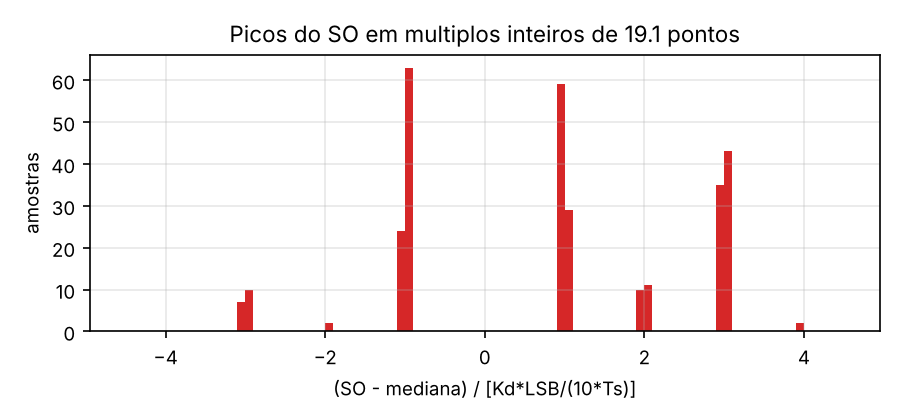
\includegraphics[width=.6\textwidth]{figs_exp/plc_histograma.png}\caption{Histograma dos picos do SO em unidades de $u_0=19{,}1$ pontos.}\end{figure}
\item \textbf{Por que há tantos picos se a VP muda devagar?} O ADC real tem ruído: quando a tensão está perto da fronteira entre dois códigos, a leitura \emph{alterna} entre eles de um scan para o outro (50 leituras por segundo). Cada alternância é um degrau de 1 LSB e gera outro pulso. No simulador fiel, um ruído de apenas $\sigma=0{,}15$ LSB ($0{,}7$ mV) reproduz a fração de picos observada:
\begin{center}\small\begin{tabular}{lccccc}\toprule $\sigma$ (LSB) & 0 & 0,10 & 0,15 & 0,20 & 0,30\\\midrule frac.\ picos (exp.: 0,20) & 0,01 & 0,18 & 0,25 & 0,39 & 0,55\\ desvio-padrão do SO (exp.: 17,3) & 2,7 & 15,0 & 16,9 & 21,6 & 26,1\\ $t_{63}$ [s] (exp.: 79) & 70 & 74 & 77 & 80 & 92\\\bottomrule\end{tabular}\end{center}
\end{enumerate}
\subsection{Terceiro: por que o SO fica entre 10 e 99,9}
Os pulsos (de até $\pm76$ pontos) somam-se ao SC e são cortados pelo \texttt{LIMIT(10,\,u,\,100)} do programa. Daí o gráfico entre 10 e 99,94\,\%. O limite inferior em 10\,\% (e não 0\,\%) é uma decisão do programa.
\subsection{Por que a planta ``não liga'' para os picos --- e por que ainda assim eles importam}
O circuito RC é um passa-baixa de 3ª ordem ($\tau\ge10$ s): pulsos de 60 ms mudam a VP em milésimos de ponto. Mas:
\begin{enumerate}
\item \textbf{Retificação pelos limites:} cortar os pulsos nos limites \emph{desloca a média} do SC. Na Q13b o SO médio no patamar saturado foi $96{,}6\,\%$ (não $99{,}94$), o que reduz a VP máxima em $\approx1{,}3$ ponto: $38{,}16$ medido contra $39{,}39$ sem ruído (Q13a). A simulação fiel prevê $38{,}35$.
\item \textbf{Congelamento da integral:} cada pulso que satura $u$ congela a integral (\texttt{STOP\_INTGR}) naquele scan: a resposta fica $\approx10\,\%$ mais lenta (t$_{63}$ 77 contra 70 s).
\item \textbf{Atuador} chaveando entre os limites; e \textbf{SC experimental não comparável} com o simulado (usa-se a mediana móvel).
\end{enumerate}
\subsection{É necessário trocar para um PI?}
\textbf{Resposta direta: não é necessário para a \emph{estabilidade}, mas é a correção mais simples; a simulação mostra que a resposta quase não muda.} Há três correções, em ordem crescente de esforço (resultados da simulação fiel ao PLC, $\sigma=0{,}15$ LSB, degrau 19,5$\to$30\,\%):
\begin{center}\small\resizebox{\textwidth}{!}{\begin{tabular}{lcccc}\toprule Programa & SO médio & desvio-padrão do SO & frac.\ picos & $t_{63}$\\\midrule
Original (\texttt{kd = 39.16}, sem filtro) & 76,1 & 16,9 & 0,25 & 77 s\\
\textbf{(1) PI de Dahlin:} \texttt{kp = 3.021}, \texttt{ki = 0.03872}, \texttt{kd = 0} & 76,1 & \textbf{0,1} & 0,00 & 71 s\\
\textbf{(2) PID com passa-baixa na VP} ($\tau_f=1{,}11$ s, só para a derivada) & 76,1 & \textbf{0,3} & 0,00 & 70 s\\
(3) só inicializar a derivada ao fechar a malha & 75,0 & 18,8 & 0,29 & 77 s\\\bottomrule\end{tabular}}\end{center}
\begin{figure}[H]\centering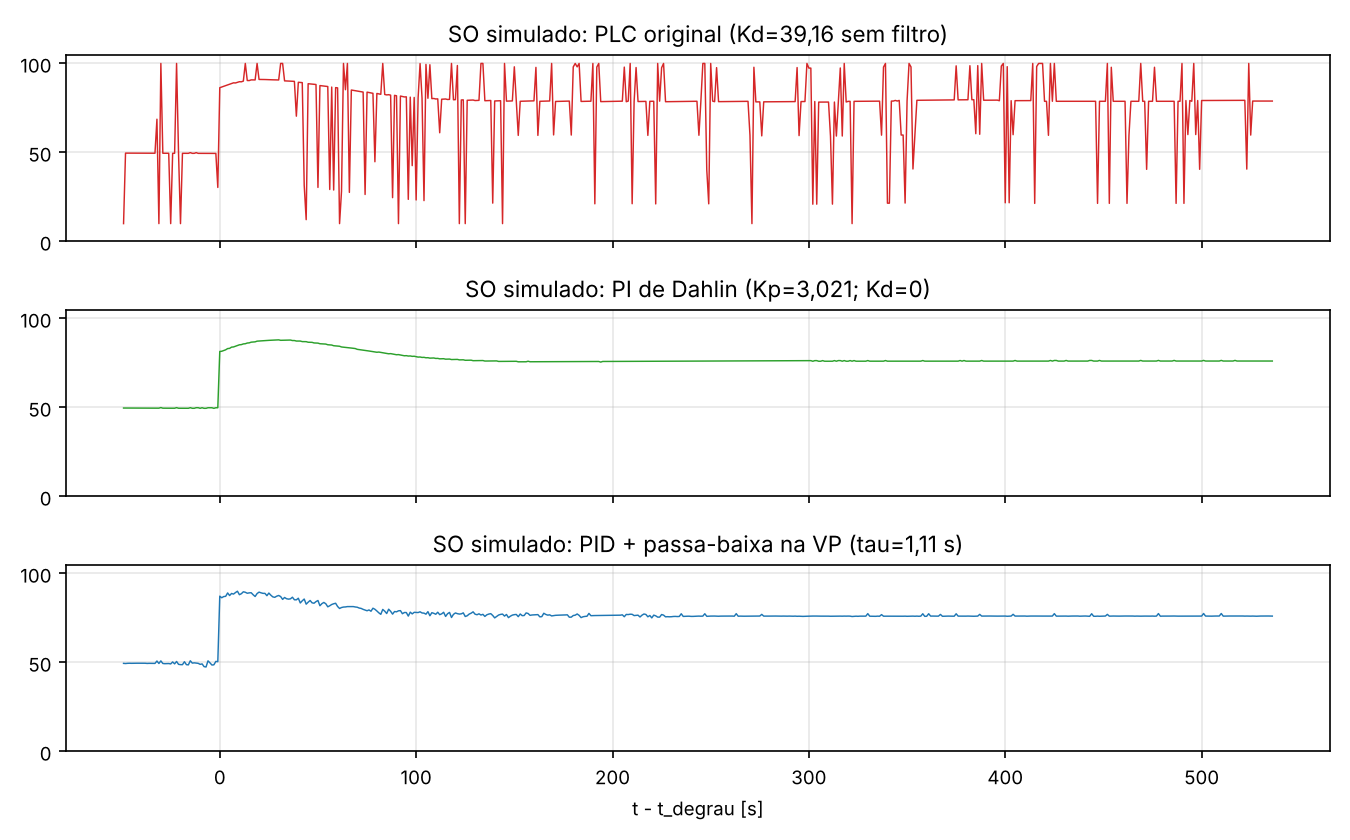
\includegraphics[width=.9\textwidth]{figs_exp/plc_correcoes.png}\caption{SO simulado (simulação fiel ao PLC): programa original, PI de Dahlin e PID com passa-baixa na VP.}\end{figure}
\textbf{(1) PI de Dahlin.} Vem da mesma dedução da Tabela 7-4.1 (Padé de ordem zero, $e^{-t_0s}\approx1-t_0s$): $C=\dfrac{\tau s+1}{Ks(\tau_c+t_0)}\Rightarrow K_c=\dfrac{\tau}{K(\tau_c+t_0)}=\dfrac{78{,}03}{0{,}3918\cdot65{,}92}=3{,}02$, $\tau_I=\tau=78{,}03$ s, \textbf{logo $k_i=K_c/\tau_I=3{,}02/78{,}03=0{,}03872$, o mesmo $k_i$ do PID}. No programa basta alterar \texttt{kp := 3.021} e \texttt{kd := 0.0}. Na FT completa, o PI dá $PM=70^\circ$ e $GM=9{,}5$ (contra $81^\circ$ e $59{,}7$ do PID), com resposta equivalente, e o efeito de 1 LSB da VP no SC cai de 76 pontos (pico da derivada de 4 pontos) para $K_c\cdot0{,}0976=0{,}3$ ponto.\\
\textbf{(2) Passa-baixa na VP antes da derivada} (mantém o PID do enunciado). Acrescentar no programa:
\begin{lstlisting}
(* variaveis novas:  VP_F : REAL := 0.0;   kf_VP : REAL := 0.017699;   (= 0.02/(1.11+0.02)) *)
IF NOT MF THEN VP_F := VP_PERC; END_IF;                       (* em manual, acompanha a VP *)
VP_F := VP_F + kf_VP * (VP_PERC - VP_F);                      (* passa-baixa de 1a ordem, Ts = 20 ms *)
Kd_VP_PERC := -1.0 * kd * VP_F * M_ACAO;                      (* no lugar de SEL(MF, 0.0, -VP*kd*M_ACAO) *)
\end{lstlisting}
O filtro é o $\mu T_d=0{,}1\cdot11{,}11=1{,}11$ s do projeto, e a linha sem \texttt{SEL(MF,\ldots)} mantém a derivada ``armada'' em manual, eliminando o pulso ao fechar a malha. \textbf{Estas duas correções foram validadas só em simulação, não na bancada.}\\
\textbf{(3)} Inicializar a derivada \emph{sozinha} não resolve o ruído (linha 3 da tabela): o problema é a falta de filtro.
\textbf{Recomendação:} (a) manter o relatório do item 1.1 como PID (é o que o enunciado pede) e documentar o ruído com esta análise; (b) \textbf{registrar um ensaio com PI} (correção 1) ou com a correção 2 e confrontar VP e SC: o SC deve ficar limpo (desvio-padrão do SO em torno de 0,1--0,3 ponto, como na simulação) e $t_{63}\approx70$ s.

%------------------------------------------------------------------
\section{Simulação fiel ao PLC (com ruído do ADC) $\times$ experimentos}\label{simplc}
Na Parte A, a simulação \emph{ideal} reproduz a VP dos ensaios com RMS de 0,24 a 0,43\,\% (exceto onde o ruído importa, Q13b), mas não reproduz três coisas: (i) o SO ruidoso, (ii) o fato de a resposta experimental ser $\approx10\,\%$ mais lenta e (iii) o deslocamento da média do SC (retificação). Para checar a explicação da Seção~\ref{expruido}, montei o \textbf{simulador fiel ao programa do PLC} (\texttt{plc\_sim.py}): a cada 20 ms ele executa o programa --- ADC de 10 bits com ruído, zona morta de $0{,}09$, integral com \texttt{STOP\_INTGR}, derivada de 4 pontos \emph{sem filtro}, bias \texttt{SO\_AUX}, \texttt{LIMIT(10,\,u,\,100)} e o 2GL por \texttt{FF2GL} --- sobre a mesma planta de 3ª ordem. O único parâmetro livre é o \textbf{ruído do ADC}, $\sigma\approx0{,}15$ LSB ($0{,}7$ mV), ajustado uma vez na Q11 e mantido nas demais.
\subsection{Q11}
\begin{figure}[H]\centering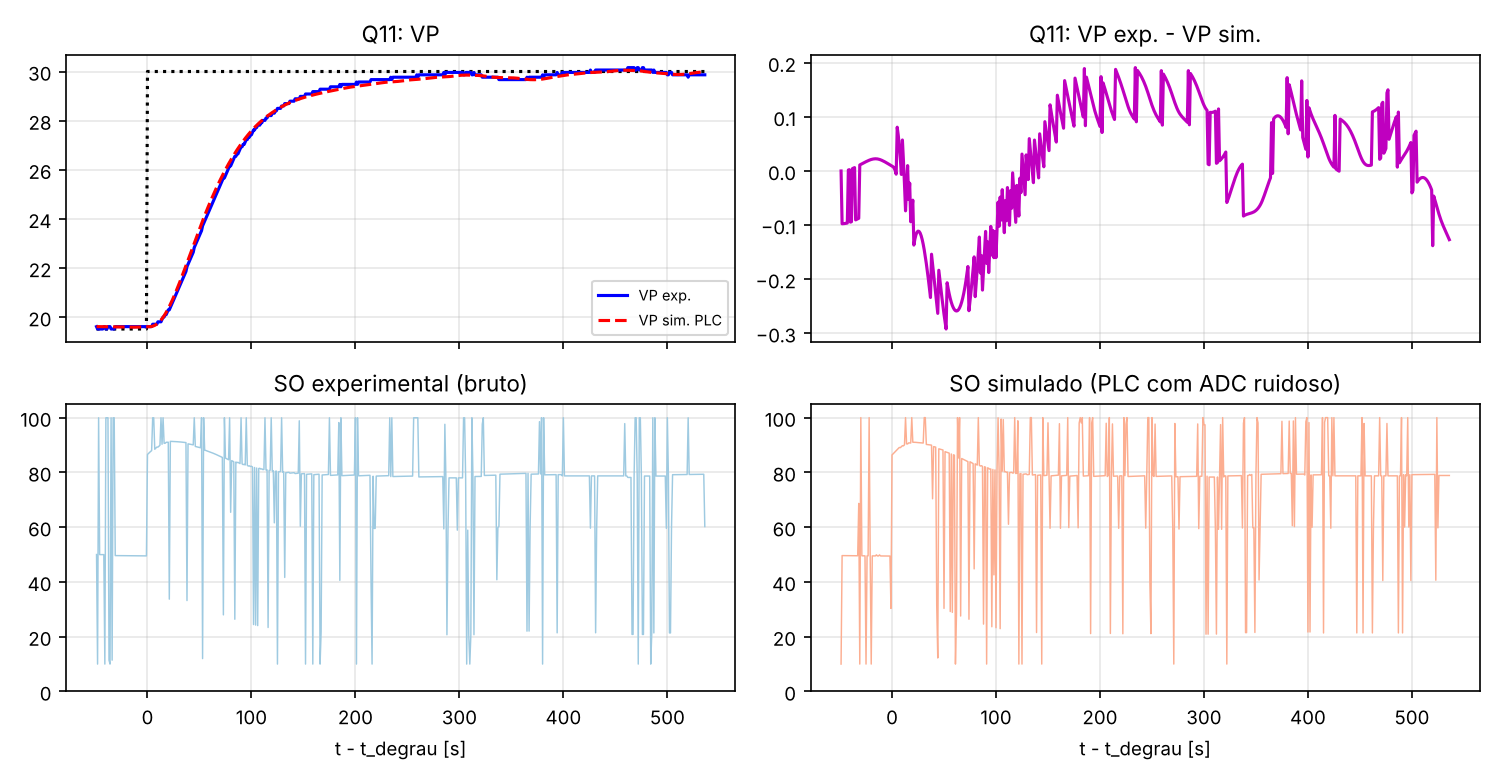
\includegraphics[width=.98\textwidth]{figs_exp/plc_q11.png}\caption{Q11 com a simulação fiel ao PLC. Acima: VP experimental, simulada e a diferença. Abaixo: SO experimental e SO simulado.}\end{figure}
\begin{center}\small
\begin{tabular}{lccc}\toprule & Experimento & Sim.\ ideal (Parte A) & Sim.\ fiel ao PLC\\\midrule
$t_{28,3}$ / $t_{50}$ / $t_{63,2}$ [s] & 43 / 64 / 79 & 39 / 57 / 70 & 41 / 62 / 77\\
$t_{90}$ / $t_{95}$ / $t_{98}$ [s] & 147 / 202 / 260 & 118 / 142 / 174 & 152 / 214 / 290\\
Erro VP: RMS / máx.\ [\%] & --- & 0,38 / 0,91 & \textbf{0,11 / 0,29}\\
SO médio em regime (últimos 300 s) & 75,4 & 76,2 & 76,1\\
Desvio-padrão do SO bruto & 17,3 & (sem ruído) & 16,9\\
Fração de amostras com pico ($|SO-\text{mediana}|>8$) & 0,20 & 0 & 0,25\\\bottomrule\end{tabular}\end{center}
A simulação fiel reduz o erro de VP em três vezes e reproduz o SO bruto em estatística (média, dispersão, fração de picos). A lentidão extra tem causa: cada pico que satura $u$ congela a integral naquele scan (\texttt{STOP\_INTGR}); sem ruído (PI ou derivada filtrada), a simulação fiel prevê $t_{63}=70$--71 s, igual à simulação ideal.
\subsection{Q12}
A simulação fiel dá, nos três primeiros scans após fechar a malha, \texttt{10, 10, 10} (derivada zerada em manual) e depois $49{,}2$; a mediana do SO de 595 a 615 s é $51{,}9$ (experimento: $50{,}2$; ideal: $49{,}2$) e a VP tem RMS de $0{,}22\,\%$ (ideal: $0{,}24\,\%$).
\subsection{Q13a e Q13b}
\begin{figure}[H]\centering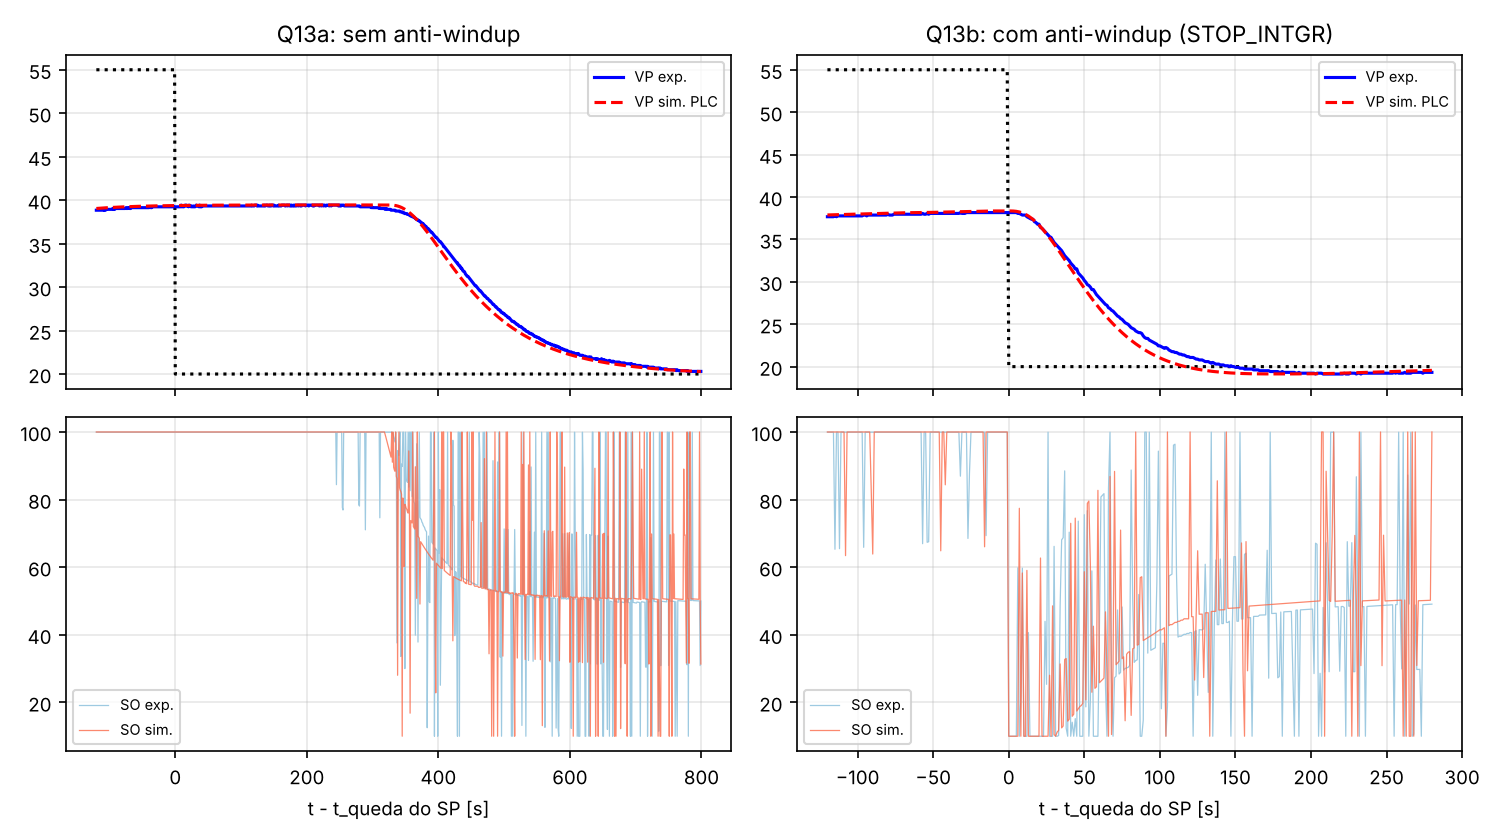
\includegraphics[width=.98\textwidth]{figs_exp/plc_q13.png}\caption{Q13 alinhado na queda do SP ($t=0$), com a simulação fiel ao PLC. Esquerda: sem anti-windup. Direita: com anti-windup (\texttt{STOP\_INTGR}). Acima: VP. Abaixo: SO experimental e simulado.}\end{figure}
\begin{center}\small
\resizebox{\textwidth}{!}{\begin{tabular}{lcccccc}\toprule & \multicolumn{3}{c}{Q13a: sem AW} & \multicolumn{3}{c}{Q13b: com AW}\\
 & Exp. & Ideal & Fiel & Exp. & Ideal & Fiel\\\midrule
O SO sai da saturação [s] & 337 & 326 & 325 & 0 & 0 & 0\\
VP em $20\pm1$ [s] & 700 & --- & 681 & 123 & --- & 101\\
SO médio no patamar saturado [\%] & 99,9 & 100,0 & 100,0 & 96,6 & 99,9 ($96{,}5^*$) & 96,5\\
VP máxima [\%] & 39,33 & 39,36 & 39,38 & 38,16 & 39,40 ($38{,}03^*$) & 38,35\\
Erro RMS da VP [\%] & --- & 0,43 & 0,44 & --- & 9,2 ($1{,}62^*$) & 0,63\\\bottomrule\end{tabular}}\end{center}
{\small $^*$ Na simulação ideal da Q13b, o limite superior do SC foi ajustado à mão a $96{,}5\,\%$ (a média medida) para emular a retificação do ruído; sem esse ajuste o RMS é 9,2\,\%. Na simulação fiel, a retificação surge sozinha do ruído do ADC.}
\par A simulação fiel reproduz os dois ensaios com a estrutura correta (sem \texttt{STOP\_INTGR} na Q13a e com na Q13b) e \emph{explica} a média de 96,6\,\% do SO e a VP máxima de 38,16 sem ajuste manual.
\subsection{O que a simulação fiel mostra}
\begin{itemize}
\item A explicação do ruído (derivada de 4 pontos sem filtro sobre o ADC) é \emph{suficiente} para reproduzir os três efeitos que a simulação ideal não captura.
\item A simulação ideal continua sendo a referência de projeto (Seções~\ref{it31}, \ref{it41} e Parte C): é nela que as sintonias são verificadas. A simulação fiel serve para \emph{prever o desvio} que o programa original causa na bancada.
\end{itemize}

\section{Comentário sobre a correção do bloco PID do OpenPLC}\label{progcorr}
\textbf{Comentário.} O bloco PID do programa (\texttt{Prova2.st}) calcula a derivada com uma diferença finita de 4 pontos a cada 20 ms \emph{sem nenhum filtro}, e ainda a zera em manual. Isso é inadequado para uma VP lida por um ADC de 10 bits: cada degrau (ou alternância) de 1 LSB vira um pulso de até $0{,}4\,k_d\,\mathrm{LSB}/T_s$ pontos no SC. A correção proposta é a que a teoria do PID prática já prevê: um \textbf{filtro derivativo} ($N$ ou $\mu$ na forma $\frac{K_ds}{\mu T_ds+1}$ das seções 7 a 13), aqui implementado como passa-baixa de 1ª ordem sobre a VP antes do bloco \texttt{DERIVATIVE}, com a mesma constante $\mu T_d=1{,}11$ s usada em todos os projetos deste relatório; e deixar a derivada ``armada'' em manual para eliminar o pulso ao fechar a malha. \textbf{O que está feito:} o texto \texttt{Prova2\_corrigido.st} e o projeto OpenPLC corrigido, com a previsão por simulação. \textbf{O que falta (a cargo do aluno):} repetir os ensaios com o programa corrigido e comparar com o programa original (Seção~\ref{simplc}) --- as caixas amarelas abaixo.
\subsection{O que mudou e o que se espera}
Gerei o arquivo \texttt{Prova2\_corrigido.st}, que é o \texttt{Prova2.st} com \textbf{duas alterações} (diferença completa em \texttt{Prova2\_diff.txt}, Apêndice~\ref{apcodigos}):
\begin{enumerate}
\item \textbf{Passa-baixa na VP antes da derivada:} \texttt{VP\_F := VP\_F + kf\_VP*(VP\_PERC - VP\_F)}, com \texttt{kf\_VP = 0.017699} $=T_s/(\tau_f+T_s)=0{,}02/(1{,}11+0{,}02)$, isto é, $\tau_f=1{,}11$ s ($=\mu T_d$ do projeto). A derivada passa a atuar sobre \texttt{VP\_F}. Em manual, \texttt{VP\_F} acompanha a VP.
\item \textbf{Derivada sem o \texttt{SEL(MF, 0.0, ...)}:} fica ``armada'' também em manual, o que elimina o pulso de 3 scans ao fechar a malha.
\end{enumerate}
Todo o resto (\texttt{kp}, \texttt{ki}, \texttt{kd}, \texttt{alfa}, \texttt{STOP\_INTGR}, \texttt{LIMIT}, VP-tracking) permanece igual. \textbf{Previsão da simulação fiel ao PLC} ($\sigma=0{,}15$ LSB; desvio-padrão do SO em $t>300$ s após o degrau) para os itens que ainda serão ensaiados:
\begin{center}\small\resizebox{\textwidth}{!}{\begin{tabular}{l|ccc|ccc|c}\toprule & \multicolumn{3}{c|}{Programa original} & \multicolumn{3}{c|}{Programa corrigido} & Projeto\\
Cenário & SO sd & sobress. & $t_{63}$ & SO sd & sobress. & $t_{63}$ & (sem ruído)\\\midrule
1.1 Dahlin, 20$\to$30\,\% & 19,9 & 0,5\,\% & 77 s & \textbf{0,2} & 0,0\,\% & 70 s & 70 s\\
2.1 2GL (\texttt{alfa=0.36}), 20$\to$30\,\% & 18,9 & 0,5\,\% & \textbf{132 s} & \textbf{0,9} & 0,0\,\% & 103 s & 104 s\\
3.1 IAE, 20$\to$25\,\% & 21,2 & 1,1\,\% & 50 s & \textbf{0,7} & 2,7\,\% & 45 s & 44 s; 2,6\,\%\\
4.1 Z--N, 10$\to$12\,\% & 28,6 & \textbf{82\,\%} & 23 s & \textbf{1,3} & 64\,\% & 21 s & 21 s; 62\,\%\\
4.2 I\_PD (\texttt{alfa=0}), 10$\to$12\,\% & 23,4 & \textbf{15,8\,\%} & 54 s & \textbf{2,6} & 0,0\,\% & 46 s & 46 s; 1,6\,\%\\\bottomrule\end{tabular}}\end{center}
\begin{res}\textbf{O programa original distorce também os ensaios que ainda faltam}: o Z--N daria 82\,\% de sobressinal em vez de 62\,\%; o I\_PD, 16\,\% em vez de $\approx2\,\%$; o 2GL ficaria em 132 s em vez de 104 s (a integral congelada pelos picos \emph{atrasa} a resposta); no Z--N e no I\_PD, com $k_d=197$, cada LSB vira pulsos de 4 vezes o tamanho (até 385 pontos). Com o programa corrigido, a simulação volta aos valores de projeto e o SO fica limpo (desvio-padrão de 0,2 a 2,6 pontos). \textbf{Recomendo usar o \texttt{Prova2\_corrigido.st} em todos os ensaios dos itens 2.1 a 4.2.}\end{res}
\subsection{O projeto OpenPLC completo (\texttt{PI\_DtwoGL\_prll\_uno\_beta}) e o projeto corrigido}\label{projplc}
Depois de analisar o \texttt{Prova2.st}, recebi a pasta completa do projeto (\texttt{plc.xml} em diagrama de blocos, mais os arquivos de compilação). Confirmei que o \texttt{Prova2.st} é exatamente o texto gerado desse diagrama e ganhei informações dos comentários e das declarações do próprio projeto:
\begin{itemize}
\item \textbf{Mapa de pinos (Arduino Uno):} \texttt{VP} = \texttt{\%IW0} = entrada analógica A0; \texttt{SO} = \texttt{\%QW1} = saída PWM do pino 10; \texttt{MF} = \texttt{\%QX0.0} = saída digital do pino 7 (``malha fechada $=1$''); \texttt{SP} = \texttt{\%QW0} (registrador alterado pelo ScadaBR). Valor inicial do \texttt{SO} $=6800$ ($\approx10{,}4\,\%$).
\item \textbf{Comentário do autor, no próprio diagrama:} ``\texttt{FILTRO DE MEDIA NA MEDIDA DE VP (???)}'', ao lado das conversões de escala: o autor já suspeitava que faltava um filtro na medida da VP, exatamente a correção proposta.
\item \textbf{Comentário sobre os ciclos:} ``\texttt{1/N, onde TIME CYCLE = N$\cdot$[TASK0 = 20 ms]; ex.: CYCLE = 100 ms então N = 5}''. Com \texttt{CYCLE = 500 ms}, $N=25$: o integrador é multiplicado por $1/N=0{,}04$ e a derivada por $N=25$, como analisei na Seção~\ref{secst}.
\item \textbf{Comentário do limite de 10\,\%:} ``\texttt{DEPENDE DO COOLER O MIN}'': o mínimo de 10\,\% do SC vem do atuador original (um \emph{cooler}/ventoinha que não gira abaixo desse valor).
\item \textbf{Comentário do 2GL:} ``\texttt{alfa = 0: I\_PD; alfa = 1: PI\_D}'', coerente com o código (peso $b=\mathtt{alfa}$). A legenda ``\texttt{FF2GL = kp*alfa*var\_SP}'' não bate com o bloco, que usa $(1-\mathtt{alfa})$; o comportamento correto é o do bloco.
\item A saída \texttt{SO} é PWM (no Uno, \texttt{analogWrite} de 8 bits, o que \emph{provavelmente} limita a resolução do SC a $100/255\approx0{,}4\,\%$; confirme).
\end{itemize}
\textbf{Projeto corrigido.} Em vez de apenas o texto \texttt{.st}, gerei o \textbf{projeto OpenPLC corrigido} (pasta \texttt{plc\_corrigido/PI\_DtwoGL\_prll\_uno\_beta\_corrigido/}, também em \texttt{.zip}), editando o diagrama do \texttt{plc.xml}: (i) uma rede nova de 5 blocos (\texttt{SUB}, \texttt{MUL}, \texttt{ADD}, \texttt{SEL}) calcula \texttt{VP\_F}, com comentário no diagrama (parte inferior); (ii) a entrada da derivada passa de \texttt{VP\_PERC} para \texttt{VP\_F}; (iii) o \texttt{SEL(MF, 0.0, \ldots)} da derivada foi removido. Duas variáveis novas foram declaradas (\texttt{VP\_F}, \texttt{kf\_VP}). Os arquivos de compilação antigos (\texttt{build/}) foram omitidos: o editor os regenera.
\textbf{Conferência feita:} (a) o XML novo é bem formado, os \texttt{localId} são únicos e todas as 166 referências de conexão existem; (b) escrevi um tradutor do diagrama para texto (\texttt{fbd\_para\_st.py}): aplicado ao \textbf{original}, ele reproduz as expressões do \texttt{Prova2.st} (ex.: \texttt{ERRO\_PERC}, \texttt{STOP\_INTGR}, \texttt{FF2GL}), o que valida o tradutor; aplicado ao \textbf{corrigido}, as \emph{únicas} saídas diferentes são \texttt{Kd\_VP\_PERC := MUL(-1.0, VP\_F, kd, M\_ACAO)} e \texttt{VP\_F := SEL(MF, VP\_PERC, ADD(VP\_F, MUL(SUB(VP\_PERC, VP\_F), kf\_VP)))}. \textbf{O que não foi possível:} abrir o projeto no OpenPLC Editor nem compilar com o \texttt{matiec} (não disponíveis aqui). Ao abrir, as linhas de conexão da rede nova podem precisar de ajuste visual; a lógica está conferida. \emph{Se o editor recusar o arquivo, use o \texttt{Prova2\_corrigido.st} como referência e refaça as 5 conexões à mão (são 8 linhas).}

\begin{todo}Abrir o projeto corrigido no OpenPLC Editor (pasta \texttt{PI\_DtwoGL\_prll\_uno\_beta\_corrigido}), \emph{Build} (confirmar que não há erro), carregar no Arduino; repetir o item 1.1 (Dahlin, 20$\to$30\,\%) e conferir: SO sem picos (desvio-padrão $\lesssim1$ ponto), SO $\approx76\,\%$ em regime, sem pulso de 10\,\% ao fechar a malha, $t_{63}\approx70$ s. Resultado: \underline{\hspace{6cm}}\end{todo}

%------------------------------------------------------------------
\section{Conclusões dos experimentos da Questão 1}\label{conclq1}
\begin{enumerate}
\item \textbf{Modelo validado no dia do ensaio:} inclinação $0{,}3963$ (teórico $0{,}3971$), offset de $-0{,}26$ ponto, dinâmica reproduzida com RMS de 0,2--0,8\,\% com o SO medido como entrada.
\item \textbf{Item 1.1 (simulação ideal):} a sintonia de Dahlin ($\tau_c=40$ s) funcionou: sem sobressinal significativo e sem erro em regime; salto de SC igual a $K_p\Delta SP$; RMS da VP de 0,38\,\%. A resposta experimental é $\approx13\,\%$ mais lenta que a ideal ($t_{63}$ de 79 contra 70 s).
\item \textbf{Item 1.2:} sem VP-tracking o SC saltou $+30$ pontos (previsto $K_p(SP-VP)=29{,}2$); com tracking (Q11), não há salto.
\item \textbf{Item 1.3:} sem anti-windup a VP fica presa em 39,3\,\% por $\approx340$ s depois da queda do SP e só chega a $20\pm1\,\%$ em 700 s; com anti-windup, em 123 s. A conta analítica dá 328 s para a saída da saturação (medido 337).
\item \textbf{SO ``instável'':} é \textbf{ruído no sinal de controle}, não instabilidade. O programa usa uma derivada de 4 pontos \emph{sem filtro} sobre a VP quantizada em 1 LSB; cada degrau (ou alternância) de 1 LSB gera pulsos de 57, 76 e 57 pontos durante 3 scans de 20 ms, cortados em 10 e 100\,\% pelo \texttt{LIMIT}. Prova: 100\,\% dos 295 picos medidos são múltiplos inteiros de $k_dLSB/(10T_s)=19{,}1$ pontos. A simulação fiel ao PLC reproduz o ruído, a lentidão e a retificação.
\item \textbf{Consequências do ruído:} retificação (SO médio de 96,6\,\% no patamar saturado), congelamento intermitente da integral (resposta $\approx10\,\%$ mais lenta) e SC experimental ruidoso.
\item \textbf{Correção do bloco PID:} passa-baixa de 1,11 s na VP antes da derivada e derivada armada em manual (\texttt{Prova2\_corrigido.st} e projeto corrigido); alternativa mínima: PI de Dahlin. \textbf{Previsão apenas por simulação; os ensaios com o programa corrigido serão feitos depois} (Seção~\ref{progcorr}).
\item \textbf{Tradução do 2GL:} no programa, $\mathtt{alfa}_{PLC}=1-\alpha_{TCC}$; o $\alpha_{TCC}=0{,}64$ do item 2.1 vira \texttt{alfa = 0.36}; o I\_PD do item 4.2 é \texttt{alfa = 0}.
\end{enumerate}
\textbf{Limitações:} (i) as versões do programa usadas em Q12 e Q13a são inferidas dos dados; (ii) o ruído do ADC é um único parâmetro ajustado ($\sigma\approx0{,}15$ LSB; faixa 0,1--0,2); (iii) a fórmula de 4 pontos do bloco \texttt{DERIVATIVE} é a da biblioteca padrão, confirmada indiretamente pelos dados e não pelo código-fonte do runtime; (iv) as correções (PI, passa-baixa e o projeto corrigido) só foram testadas em simulação e não foram compiladas no OpenPLC; (v) um ensaio de cada tipo, sem repetição.


%==================== PARTE C: QUESTÕES 3 E 4 (PREPARAÇÃO EXPERIMENTAL) ====================
\section{Questões 3 e 4: preparação experimental (a realizar)}\label{q34}
Esta parte segue o \textbf{mesmo padrão} dos itens da Questão 1 (Seções~\ref{expq11} a \ref{expq13}): objetivo e fundamentos, como digitar a sintonia no programa do PLC, procedimento, \textbf{previsão da simulação ideal} (planta completa, sem ruído do ADC, com os limites do SC do programa), planilha de resultados a preencher, roteiro de interpretação e riscos. Os ensaios dos itens 3.1, 4.1 e 4.2 \textbf{serão realizados depois}; as caixas amarelas e as tabelas ``Experimento'' ficam em branco para serem preenchidas. A teoria e os cálculos das sintonias estão nas Seções~\ref{it31} e \ref{it41}; o item 4.2 (I\_PD) é desenvolvido aqui.

\subsection{Roteiro comum aos ensaios}\label{roteirocomum}
\begin{enumerate}
\item \textbf{Programa.} Usar o \texttt{Prova2\_corrigido.st} (projeto corrigido, Seção~\ref{progcorr}) \emph{ou}, se for repetir exatamente os ensaios da Questão 1, o \texttt{Prova2.st}. Com a derivada sem filtro do programa original, os ganhos $k_d$ destes itens ($71{,}6$ e $197{,}3$) geram pulsos de 140 e 385 pontos por LSB da VP (Seção~\ref{expruido}), e o SO fica saturado em 10 e 100\,\%; os resultados experimentais seriam distorcidos.
\item \textbf{Condição inicial (manual).} $SO_0=\dfrac{SP_0+0{,}262}{0{,}3963}$ (inversa do ajuste da Seção~\ref{expplanta}); esperar $\ge8$ min ($\ge7\tau_1$) até a VP estabilizar em $SP_0$. Em manual o programa faz $SP=VP$ (VP-tracking), então o SP já fica igual à VP no instante de fechar a malha.
\item \textbf{Fechar a malha} (\texttt{MF := 1}) com $SP=VP$; aguardar 50 s; \textbf{aplicar o degrau de SP}; gravar até a VP assentar (400--700 s).
\item \textbf{Registro:} ScadaBR a 1 s, pontos SO, SP, VP, VP1, VP2. Anotar a versão do programa, os valores digitados e os instantes das ações.
\item \textbf{Comparação:} \texttt{python3 codigos/simula\_bancada.py comparar ARQUIVO.csv --inicio <t\_fechamento> --kp .. --ti .. --td .. --sat --aw clamp} (RMS e erro máximo de VP e de SC, com a mediana móvel do SO). A tabela ``Experimento'' de cada item usa as mesmas métricas da Questão 1: sobressinal, $t_{63,2}$, tempo de acomodação ($\pm2\,\%$ do degrau), pico e valor final do SC, RMS e erro máximo da VP.
\end{enumerate}
\begin{just}\textbf{Por que estas escolhas.} A condição inicial longa evita que o transitório do circuito contamine o degrau (o polo dominante é $\tau_1=68{,}7$ s). O degrau é pequeno porque o SC tem limites $[10;100]\,\%$ e o salto proporcional $K_p\Delta SP$ é grande nestas sintonias. O $SC_0$ inclui o offset ($-0{,}262$) medido no dia dos ensaios.\end{just}

%------------------------------------------------------------------
\section{Item 3.1 (Questão 3): integral do erro mínimo (seção 7-2.3)}\label{q31exp}
\subsection{Objetivo e fundamentos}
Verificar experimentalmente a sintonia do PID pelas correlações de IAE mínimo para \emph{ponto fixo} (Tabela 7-2.3, Rovira), calculadas na Seção~\ref{it31} com $K=0{,}3918$, $\tau=78{,}03$ s, $t_0=25{,}92$ s ($r=t_0/\tau=0{,}3322$):
\[
K_c=\frac{1{,}086}{K}r^{-0{,}869}=7{,}222,\qquad\tau_I=\frac{\tau}{0{,}740-0{,}130r}=111{,}98\ \mathrm{s},\qquad\tau_D=0{,}348\,\tau\,r^{0{,}914}=9{,}92\ \mathrm{s}.
\]
Estas tabelas já dão o PID na forma \emph{ideal} (paralela), então $K_p=K_c$, $K_i=K_c/\tau_I=0{,}06449$ e $K_d=K_c\tau_D=71{,}63$ (sem conversão série$\to$ideal). A sintonia minimiza $\int|e|\,dt$ para um degrau de SP, \emph{sem penalizar o esforço de controle}: espera-se resposta rápida, algum sobressinal e SC com pico grande.
\subsection{Como digitar no programa}
\begin{center}\small\begin{tabular}{lcccc}\toprule \texttt{kp} & \texttt{ki} & \texttt{kd} & \texttt{alfa} & degrau de SP\\\midrule 7.222 & 0.06449 & 71.63 & 1.0 (PI\_D) & $20\to25\,\%$\\\bottomrule\end{tabular}\end{center}
$SO_0=(20+0{,}262)/0{,}3963=51{,}1\,\%$; $SO$ final esperado $=(25+0{,}262)/0{,}3963=63{,}7\,\%$.
\subsection{Previsão da simulação ideal}
\begin{figure}[H]\centering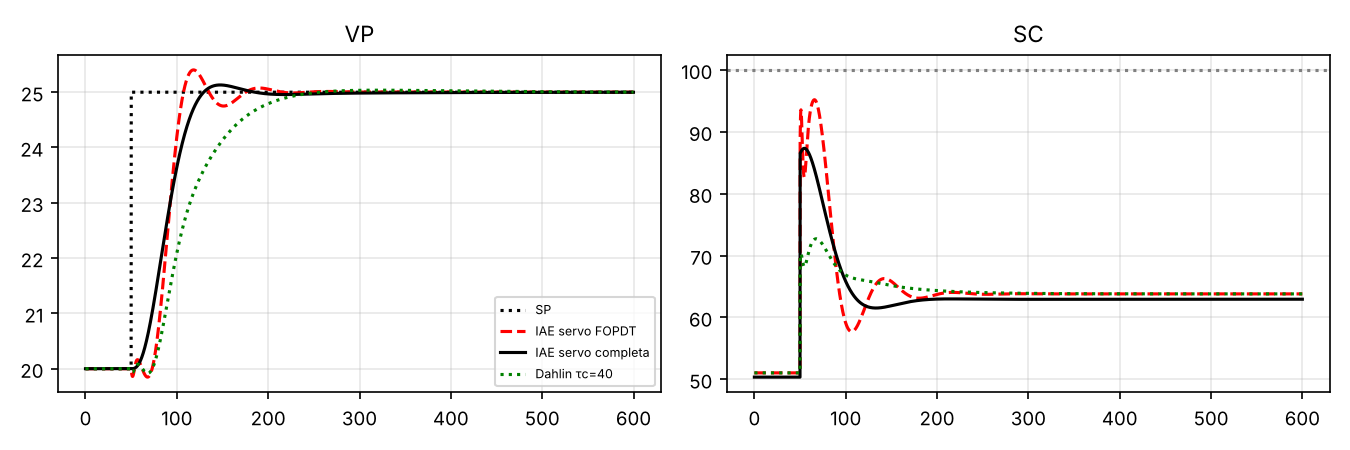
\includegraphics[width=.98\textwidth]{figs/i31.png}\caption{Item 3.1, simulação ideal: IAE ponto fixo (FOPDT tracejado vermelho; FT completa preto) e Dahlin $\tau_c=40$ s do item 1.1 (verde pontilhado), degrau $20\to25\,\%$.}\end{figure}
\begin{center}\small
\begin{tabular}{lccc}\toprule Métrica & Ideal FOPDT & Ideal FT completa & \textbf{Experimento}\\\midrule
Sobressinal [\%] & 8,1 & 2,6 & \underline{\hspace{1.6cm}}\\
$t_{63,2}$ [s] & 44 & 44 & \underline{\hspace{1.6cm}}\\
Tempo de acomodação ($\pm2\,\%$) [s] & 117 & 110 & \underline{\hspace{1.6cm}}\\
Pico do SC [\%] & 95 & 87 & \underline{\hspace{1.6cm}}\\
SC final [\%] & 63,8 & 62,9 & \underline{\hspace{1.6cm}}\ (previsto 63,7)\\
Salto do SC em $t=50$ s [pontos] & \multicolumn{2}{c}{$K_p\Delta SP=7{,}222\cdot5=36{,}1$} & \underline{\hspace{1.6cm}}\\
Erro VP: RMS / máx.\ [\%] & --- & --- & \underline{\hspace{1.6cm}}\\\bottomrule\end{tabular}\end{center}
Margens da malha aberta com esta sintonia: FOPDT $GM=1{,}9$, $PM=64^\circ$; FT completa $GM=32{,}0$, $PM=71^\circ$. Para comparação, a sintonia de \emph{distúrbio} (Tabela 7-2.2, $K_p=10{,}1$) aplicada a um degrau de SP daria sobressinal de 84\,\% (FOPDT) e 42\,\% (completa).
\subsection{Roteiro de interpretação (o que escrever)}
\begin{itemize}
\item \textbf{Salto de SC:} confira $\Delta SC(0^+)=K_p\Delta SP=36{,}1$ (como na Q11: previsto 36,9, medido 37,0). Isso confirma $K_p$ digitado.
\item \textbf{Mais rápida que o Dahlin do 1.1:} $t_{63}\approx44$ s contra $\approx70$ s; o custo é o sobressinal (2,6\,\% a 8,1\,\%) e o pico de SC ($\approx87\,\%$, perto do limite de 100).
\item \textbf{FOPDT $\times$ completa:} a diferença de sobressinal (8,1 contra 2,6\,\%) vem do atraso puro da FOPDT (menor margem de ganho). O experimento deve ficar \emph{perto da FT completa}.
\item \textbf{Diferenças esperadas na bancada} (Questão 1): resposta $\sim10\,\%$ mais lenta que a simulação ideal (tolerâncias de $R$ e $C$; ruído do SO). Com o programa original, $k_d=71{,}63$ gera pulsos de $0{,}4\cdot71{,}63\cdot0{,}0976/0{,}02=140$ pontos por LSB (saturam em 10 e 100\,\%) e o SO médio se desloca; por isso a recomendação do programa corrigido.
\end{itemize}
\begin{todo}Executar o item 3.1 conforme o roteiro (Seção~\ref{roteirocomum}) e preencher a tabela. Anotar: versão do programa, \texttt{kp}, \texttt{ki}, \texttt{kd}, \texttt{alfa}, $SO_0$ e instantes. Comparar VP e SC (figuras VP exp.\ $\times$ ideal e SC exp.\ $\times$ ideal). Resultados: \underline{\hspace{6cm}}\end{todo}

%------------------------------------------------------------------
\section{Item 4.1 (Questão 4): Ziegler--Nichols, razão de decaimento 1/4 (Tabela 7-1.1)}\label{q41exp}
\subsection{Objetivo e fundamentos}
O método usa o \textbf{ganho final} $K_{cu}$ e o \textbf{período final} $T_u$ medidos \emph{na planta real}: com controle só proporcional, aumenta-se $K_c$ até a VP oscilar com amplitude constante. Para o PID (forma real/série): $K_c'=K_{cu}/1{,}7$, $\tau_I'=T_u/2$, $\tau_D'=T_u/8$; na forma ideal, $K_p=0{,}735K_{cu}$, $T_i=0{,}625T_u$, $T_d=0{,}1T_u$ (dedução na Seção~\ref{it41}). Pela FT completa (Routh): $K_{cu}=38{,}97$, $T_u=68{,}85$ s.
\subsection{Parte 1: teste de ganho final}
\textbf{Programa:} \texttt{ki := 0.0; kd := 0.0; alfa := 1.0;} e \texttt{kp} variável (controle só proporcional). A integral é zerada em manual e com \texttt{ki=0} fica nula; o termo $SO_{man}$ (\texttt{SO\_AUX}) fixa o ponto de operação.
\textbf{Ponto de operação e degrau.} A oscilação sustentada em $K_{cu}$ tem amplitude $\approx0{,}9$ ponto por 1\,\% de degrau, e o SC oscila $\pm K_{cu}\cdot0{,}9\approx\pm35$ pontos. Para que o SC \emph{não sature} (limites 10 e 100), use $SP_0=20\,\%$ ($SO_0=51{,}1\,\%$) com degrau de \textbf{$+1$ ponto} (20$\to$21): o SC oscila entre $\approx17$ e $\approx85\,\%$.
\textbf{Procedimento:}
\begin{enumerate}
\item Fechar a malha com $SP=VP=20$ e \texttt{kp := 15}. Aplicar $SP=21$ e observar 5 ciclos.
\item Aumentar \texttt{kp} (15, 25, 30, 35, 37, 39, 41\ldots; passos menores perto de 39). Com cada valor, esperar a oscilação se estabelecer (3--4 períodos).
\item $K_{cu}$ é o \textbf{menor} \texttt{kp} para o qual a amplitude fica constante (variação $<5\,\%$ entre três picos consecutivos). Com $K_c<K_{cu}$ a oscilação amortece; com $K_c>K_{cu}$ ela cresce até a saturação.
\item $T_u$: média dos intervalos entre picos consecutivos de pelo menos 4 ciclos (o ScadaBR tem resolução de 1 s; erro de cerca de 1,5\,\%).
\end{enumerate}
\begin{figure}[H]\centering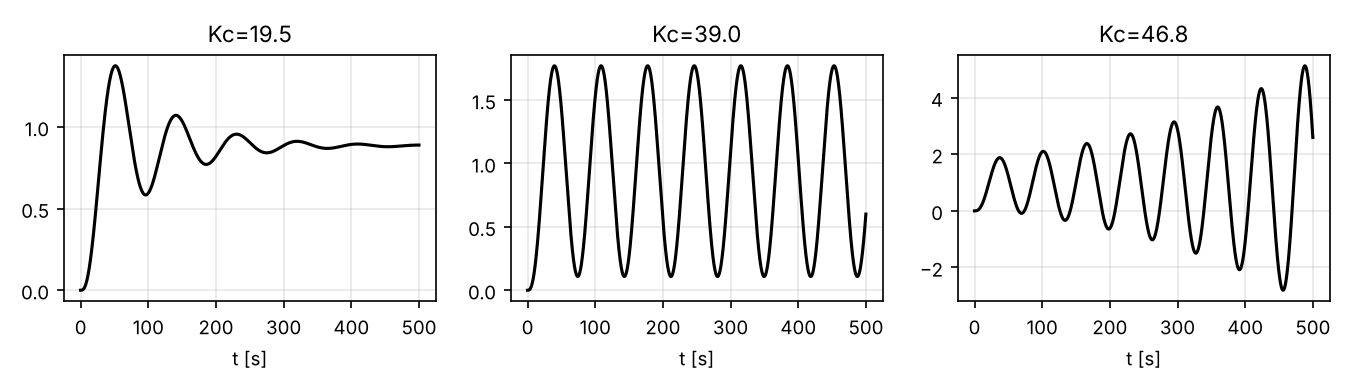
\includegraphics[width=.95\textwidth]{figs/i41_kcu.png}\caption{Teste de ganho final, simulação ideal (FT completa, controle P puro): com $0{,}5K_{cu}$ a oscilação amortece; com $K_{cu}$ é sustentada com período $T_u=68{,}85$ s; com $1{,}2K_{cu}$ cresce.}\end{figure}
\begin{center}\small
\begin{tabular}{lcc}\toprule & Previsão (FT completa) & \textbf{Experimento}\\\midrule
$K_{cu}$ & 38,97 (FOPDT daria 13,7) & \underline{\hspace{1.6cm}}\\
$T_u$ [s] & 68,85 (FOPDT daria 92,7) & \underline{\hspace{1.6cm}}\\
Amplitude da VP em $K_{cu}$ (degrau de 1 ponto) & $\approx0{,}9$ ponto & \underline{\hspace{1.6cm}}\\\bottomrule\end{tabular}\end{center}
\begin{just}Usa-se a FT \emph{completa} (e não a FOPDT) porque o Z--N exige o comportamento real no limite de estabilidade: a FOPDT subestima $K_{cu}$ em $\approx65\,\%$ (Seção 6.2). Valores medidos costumam diferir 5--15\,\% da previsão (ganho real, atraso do ciclo do PLC, quantização).\end{just}
\subsection{Parte 2: PID de Ziegler--Nichols}
Recalcular com os \emph{seus} $K_{cu}$ e $T_u$: $K_p=0{,}735K_{cu}$, $T_i=0{,}625T_u$, $T_d=0{,}1T_u$, $K_i=K_p/T_i$, $K_d=K_pT_d$. Com os valores previstos: $K_p=28{,}65$; $T_i=43{,}03$ s; $T_d=6{,}885$ s; \textbf{\texttt{kp := 28.65; ki := 0.6659; kd := 197.3; alfa := 1.0}}.
\textbf{Degrau:} como o SC pode saturar com este ganho, simulei o PID de Z--N na planta completa com os limites do programa para três pontos de operação:
\begin{center}\small\begin{tabular}{lcccc}\toprule Degrau de SP & SC mínimo & SC máximo & sobressinal & situação\\\midrule
$10\to12\,\%$ & 10,0 (satura; sem limite seria 5,5) & 86,1 & 65\,\% & \textbf{satura no limite inferior}\\
$15\to17\,\%$ & 13,6 & 98,7 & 64\,\% & no limite superior\\
$20\to22\,\%$ & 31,9 & 99,9 (sem limite: 108) & 45\,\% & \textbf{satura no superior}\\
$20\to21\,\%$ & 38,6 & 81,1 & 64\,\% & \textbf{não satura}\\\bottomrule\end{tabular}\end{center}
\textbf{Recomendação: $20\to21\,\%$} (o mesmo ponto de operação do teste de ganho final). O degrau de $10\to12$ usado na Seção~\ref{it41} (simulação sem os limites do programa) satura o SC em 10\,\%.
\subsection{Previsão da simulação ideal e planilha}
\begin{figure}[H]\centering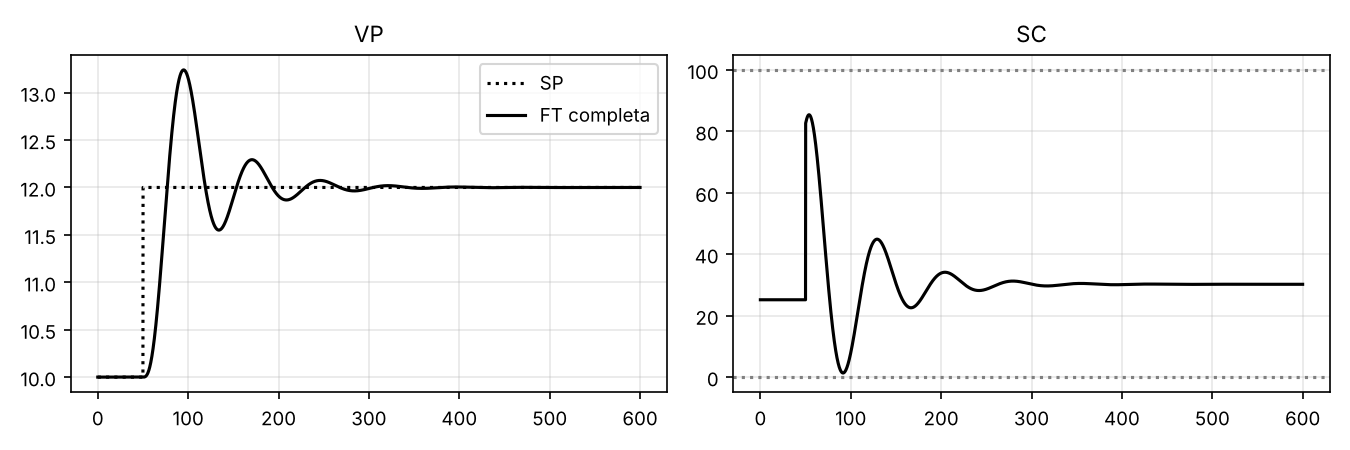
\includegraphics[width=.98\textwidth]{figs/i41.png}\caption{Item 4.1, simulação ideal (FT completa, degrau $10\to12$, sem os limites do programa): sobressinal $\approx62\,\%$ e razão de decaimento $\approx1/4$.}\end{figure}
\begin{center}\small
\begin{tabular}{lcc}\toprule Métrica (degrau $20\to21$, FT completa, com limites do programa) & Ideal & \textbf{Experimento}\\\midrule
Sobressinal [\%] & 64 & \underline{\hspace{1.6cm}}\\
$t_{63,2}$ [s] & 21 & \underline{\hspace{1.6cm}}\\
Tempo de acomodação ($\pm2\,\%$) [s] & 240 & \underline{\hspace{1.6cm}}\\
Razão de decaimento (2º pico/1º pico) & 0,24 ($\approx1/4$) & \underline{\hspace{1.6cm}}\\
SC: mínimo / máximo / final [\%] & 38,6 / 81,1 / 53,5 & \underline{\hspace{1.6cm}}\\
Salto do SC em $t=50$ s [pontos] & $K_p\Delta SP=28{,}7$ & \underline{\hspace{1.6cm}}\\
Margens da malha aberta (FT completa) & $GM=7{,}8$; $PM=22^\circ$ & ---\\\bottomrule\end{tabular}\end{center}
\begin{figure}[H]\centering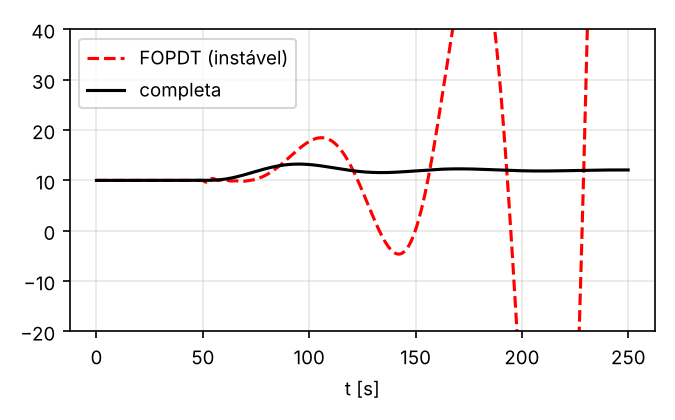
\includegraphics[width=.5\textwidth]{figs/i41_unst.png}\caption{O mesmo PID aplicado à FOPDT (instável) e à FT completa: por isso o item 4.1 só é simulado com a planta completa.}\end{figure}
\subsection{Roteiro de interpretação}
\begin{itemize}
\item \textbf{Razão de decaimento:} meça o 1º e o 2º picos acima do SP final (excesso); a razão esperada é $\approx0{,}24$. O método ``\emph{falha}'' se a razão ficar muito diferente de $1/4$ (por exemplo, por $K_{cu}$ e $T_u$ mal medidos).
\item \textbf{Sobressinal grande ($\approx64\,\%$)} é característico da razão 1/4 e da margem de fase baixa ($22^\circ$).
\item \textbf{Por que não simular com a FOPDT:} os polos de malha fechada ficam no semiplano direito ($+0{,}027\pm0{,}087j$): é instável.
\item \textbf{Ruído:} $k_d=197{,}3$ é o caso mais crítico do programa original (pico de 385 pontos por LSB). Na simulação fiel ao PLC, o programa original daria sobressinal de 82\,\% em vez de 62--64\,\% (Seção~\ref{progcorr}). Use o programa corrigido.
\end{itemize}
\begin{todo}(1) Teste de ganho final: anotar $K_{cu}$ e $T_u$ medidos. (2) Recalcular $K_p$, $K_i$, $K_d$ e digitar. (3) Degrau $20\to21\,\%$; gravar. (4) Preencher a tabela e comparar VP e SC com a simulação. Resultados: \underline{\hspace{6cm}}\end{todo}

%------------------------------------------------------------------
\section{Item 4.2 (Questão 4): I\_PD com a sintonia do 4.1}\label{q42exp}
\subsection{Objetivo e teoria}
``Aproveite a sintonia do PID para realizar um I\_PD, e explique o que acontece.'' No I\_PD, \textbf{só o integrador atua sobre o erro}; o proporcional e o derivativo atuam sobre a \emph{VP}:
\[
U(s)=\frac{K_i}{s}\big(R-Y\big)-\Big(K_p+D(s)\Big)Y,\qquad D(s)=\frac{K_d\,s}{\mu T_ds+1}\ \ (\text{no programa: derivada de 4 pontos}).
\]
Como $Y=GU$, isolando $U$ e $Y$:
\[
\frac{Y}{R}=\frac{\dfrac{K_i}{s}\,G}{1+(PI+D)\,G},\qquad\frac{U}{R}=\frac{\dfrac{K_i}{s}}{1+(PI+D)\,G},\qquad PI=K_p+\frac{K_i}{s}.
\]
Comparando com o PI\_D ($Y/R=\frac{PI\,G}{1+(PI+D)G}$):
\begin{itemize}
\item \textbf{O denominador é o mesmo} $\Rightarrow$ os mesmos polos de malha fechada (mesma estabilidade e a mesma resposta a \emph{distúrbio}, $VP/D=\frac{G}{1+(PI+D)G}$).
\item \textbf{O numerador muda:} de $(K_ps+K_i)/s$ para $K_i/s$: \textbf{o zero do PI desaparece}. O zero do PI é o responsável pelo ``chute'' proporcional ($\Delta SC(0^+)=K_p\Delta SP$) e por grande parte do sobressinal.
\item \textbf{Valor inicial:} $\Delta SC(0^+)=0$ (o SC não tem salto no degrau de SP) e o SC cresce só pela integral.
\end{itemize}
\textbf{No programa:} \texttt{alfa := 0.0}. Com $\mathtt{alfa}=0$, a \texttt{FF2GL} acumula $K_p\Delta SP$ e é subtraída de $u$, cancelando o proporcional sobre o SP (peso $b=\mathtt{alfa}=0$, Seção~\ref{alfaplc}); a integral continua sobre o erro completo e a derivada, sobre a VP.
\subsection{Como digitar e procedimento}
Mesmos parâmetros do 4.1 (com os $K_{cu}$ e $T_u$ medidos): \texttt{kp := 28.65; ki := 0.6659; kd := 197.3; \textbf{alfa := 0.0}}. Procedimento do roteiro comum (Seção~\ref{roteirocomum}), degrau $20\to22\,\%$ (o I\_PD não tem salto de SC, então o limite de 100\,\% não é problema). Se houver tempo, sobrepor com o ensaio PI\_D do 4.1.
\subsection{Previsão da simulação ideal}
\begin{figure}[H]\centering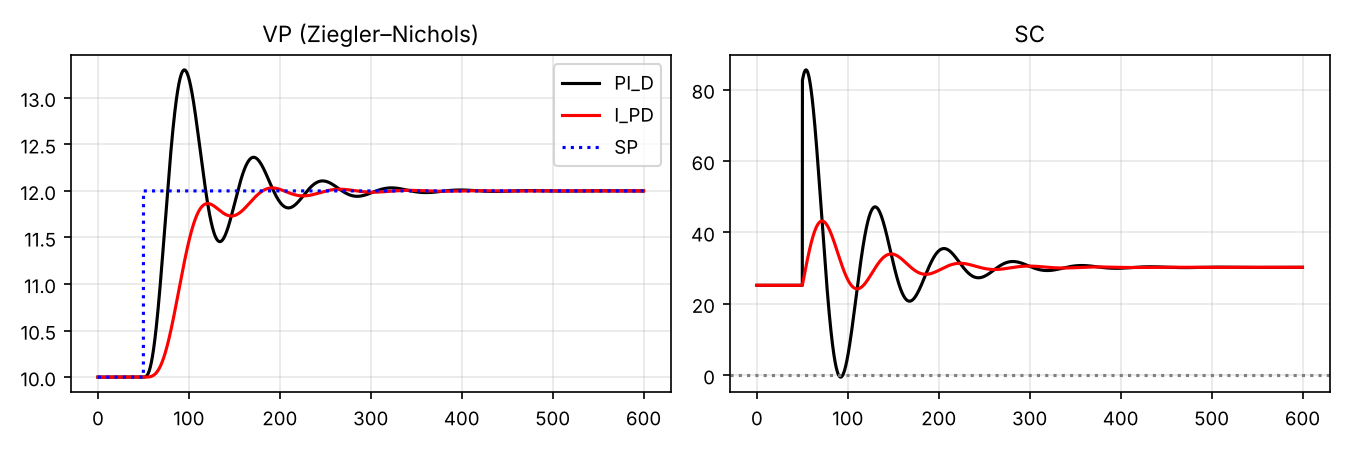
\includegraphics[width=.98\textwidth]{figs/g42.png}\caption{Item 4.2, simulação ideal (FT completa): PI\_D (preto) e I\_PD (vermelho) com a sintonia de Z--N, degrau $10\to12\,\%$.}\end{figure}
\begin{center}\small
\begin{tabular}{lccc}\toprule Métrica (FT completa, Z--N, com limites do programa) & PI\_D (4.1) & I\_PD ideal & \textbf{I\_PD experimento}\\\midrule
Sobressinal [\%] & 64--65 & 1,2 & \underline{\hspace{1.4cm}}\\
$t_{63,2}$ [s] & 21 & 46 & \underline{\hspace{1.4cm}}\\
Tempo de acomodação ($\pm2\,\%$) [s] & 210--240 & 183 & \underline{\hspace{1.4cm}}\\
Salto do SC em $t=50$ s [pontos] & $+28{,}7$ ($K_p\Delta SP$, 1 ponto) & \textbf{0} & \underline{\hspace{1.4cm}}\\
SC ($20\to22$): mínimo / máximo [\%] & 31,9 / 99,9 (satura) & 50,3 / 68,9 & \underline{\hspace{1.4cm}}\\\bottomrule\end{tabular}\end{center}
Para a sintonia de Dahlin (item 1.1) com I\_PD (degrau $20\to30$): sobressinal 0\,\%, $t_{63}=164$ s (contra 70 s do PI\_D), tempo de acomodação 434 s, SC máximo 76,2\,\% (sem pico: o SC sobe monotonicamente ao valor final, contra o pico de 88,6\,\% do PI\_D). Com a sintonia IAE do 3.1, o I\_PD (degrau $20\to25$) dá 0\,\% de sobressinal e $t_{63}=151$ s, contra 44 s do PI\_D.
\subsection{Roteiro de interpretação (``explique o que acontece'')}
\begin{enumerate}
\item \textbf{Menor sobressinal e SC suave:} o I\_PD elimina o zero do PI e o salto proporcional; a VP sobe sem o ``chute'' inicial.
\item \textbf{Mais lento:} sem a ação proporcional ``antecipada'' no SP, $t_{63}$ passa de 21 para 46 s (Z--N). Isso é o preço da suavidade.
\item \textbf{Mesma estabilidade e mesma rejeição de distúrbio:} o denominador não mudou ($PM=22^\circ$ e $GM=7{,}8$ iguais). Um distúrbio ($R_p$) teria a mesma resposta nos dois casos.
\item \textbf{Quando usar:} com ganho alto e atuador sensível a degraus de SP, ou para evitar saturação em mudanças de SP (a Tabela mostra o PI\_D saturando em $20\to22$, o I\_PD não).
\item \textbf{Relação com o 2GL:} I\_PD é o caso $b=0$ ($\mathtt{alfa}=0$); PI\_D, $b=1$ ($\mathtt{alfa}=1$); os valores intermediários são o PID 2GL do item 2.1.
\end{enumerate}
\begin{todo}Executar o I\_PD com \texttt{alfa := 0.0} (mesmos \texttt{kp}, \texttt{ki}, \texttt{kd} do 4.1) e preencher a tabela. Conferir: salto de SC $\approx0$; sobressinal $\lesssim2\,\%$; $t_{63}\approx46$ s. Comparar com o ensaio PI\_D do 4.1. Resultados: \underline{\hspace{6cm}}\end{todo}

%------------------------------------------------------------------
\section{Quadro dos ensaios}\label{quadro}
\begin{center}\small
\resizebox{\textwidth}{!}{\begin{tabular}{llllll}\toprule Item & Programa/parâmetros & Degrau & Previsão ideal & Experimento & Seção\\\midrule
1.1 & \texttt{kp 3.523; ki 0.03872; kd 39.16; alfa 1} & $19{,}5\to30$ & $t_{63}=70$ s; 0\,\% & realizado (Q11) & \ref{expq11}\\
1.2 & idem, sem VP-tracking & $SP\ne VP$ & salto $=K_p(SP-VP)$ & realizado (Q12) & \ref{expq12}\\
1.3 & idem, sem/com \texttt{STOP\_INTGR} & $25\to55\to20$ & saída da sat.\ $\approx$ 330 s / 0 & realizado (Q13a, b) & \ref{expq13}\\
2.1 & \texttt{kp 5.057; ki 0.05558; kd 56.21; alfa 0.36} & $20\to30$ & $t_{63}=104$ s; 0\,\% & \textbf{a realizar} & \ref{it21}\\
2.2 & idem, com $R_p=133{,}6$ k$\Omega$ & distúrbio & queda 2,6 pt; 134 s & \textbf{a realizar} & ---\\
3.1 & \texttt{kp 7.222; ki 0.06449; kd 71.63; alfa 1} & $20\to25$ & 2,6\,\%; $t_{63}=44$ s & \textbf{a realizar} & \ref{q31exp}\\
4.1 & ganho final; depois \texttt{kp 28.65; ki 0.6659; kd 197.3} & $20\to21$ & 64\,\%; $t_{63}=21$ s & \textbf{a realizar} & \ref{q41exp}\\
4.2 & idem 4.1, \texttt{alfa 0} & $20\to22$ & 1,2\,\%; $t_{63}=46$ s & \textbf{a realizar} & \ref{q42exp}\\\bottomrule\end{tabular}}\end{center}

%==================== APÊNDICE: CÓDIGOS ====================
\appendix
\section{Códigos usados na comparação experimento $\times$ simulação}\label{apcodigos}
Todos os arquivos estão na pasta \texttt{codigos/} desta entrega (dados em \texttt{dados/}). Para reproduzir os números e as figuras da Seção~14 em diante, a partir da pasta \texttt{entrega/}: \texttt{python3 codigos/analise\_experimentos.py} (precisa de \texttt{numpy}, \texttt{scipy} e \texttt{matplotlib}).
\begin{center}\small\begin{tabular}{lp{10.5cm}}\toprule Arquivo & Função\\\midrule
\texttt{load\_q.py} & Leitura do CSV do ScadaBR (formato longo) e alinhamento das 5 variáveis numa grade de 1 s\\
\texttt{simexp.py} & Simulador de malha fechada (planta de 3ª ordem completa, PI\_D, saturação, anti-windup, offset)\\
\texttt{analise\_experimentos.py} & Análise dos ensaios Q11, Q12, Q13a e Q13b: métricas, estatística do ruído, PI $\times$ PID e figuras\\
\texttt{simula\_bancada.py} & Ferramenta de linha de comando para comparar \emph{qualquer} ensaio (RMS de VP e SC), com opções de $\alpha$, I\_PD, saturação, anti-windup e $R_p$\\
\texttt{compara\_malha.m} & Versão em MATLAB (estilo do script do professor), \textbf{não executada}\\\bottomrule\end{tabular}\end{center}
\subsection{\texttt{load\_q.py}: leitura dos dados}
\lstinputlisting[language=Python]{codigos/load_q.py}
\subsection{\texttt{simexp.py}: simulador de malha fechada}
\lstinputlisting[language=Python]{codigos/simexp.py}
\subsection{\texttt{analise\_experimentos.py}: análise dos ensaios}
\lstinputlisting[language=Python]{codigos/analise_experimentos.py}
\subsection{\texttt{simula\_bancada.py}: comparação genérica}
\lstinputlisting[language=Python]{codigos/simula_bancada.py}
\subsection{\texttt{compara\_malha.m}: versão MATLAB}
\lstinputlisting[language=Matlab]{codigos/compara_malha.m}

\end{document}
